% !Mode:: "TeX:UTF-8"
% !TEX TS-program = xelatex
% !TEX program = xelatex
% WinEdt: compile with XeLaTeX (recommended) or PDFLaTeX.
% ============================================================
% LINEAR ALGEBRA -- MAIN FILE
% Compile:          latexmk main.tex   (XeLaTeX, via latexmkrc)
% A single chapter: latexmk boblar/bob3.tex
% ============================================================
\documentclass[10pt, a5paper, twoside, openright]{book}
% !Mode:: "TeX:UTF-8"
% ============================================================
% BOOK DATA
% The title page, the page headers and the imprint page take their
% text from here; editing this file is enough.
% ============================================================

\newcommand{\KitobNomi}{Linear Algebra}
\newcommand{\KitobNomiKatta}{LINEAR ALGEBRA}
\newcommand{\KitobTuri}{Study Guide}

\newcommand{\Muallif}{Nodirjon I. Tolipov}
\newcommand{\MuallifQisqa}{N.\,I.~Tolipov}

\newcommand{\Vazirlik}{MINISTRY OF HIGHER EDUCATION, SCIENCE AND INNOVATION\\OF THE REPUBLIC OF UZBEKISTAN}
\newcommand{\Muassasa}{FERGANA STATE TECHNICAL UNIVERSITY}

\newcommand{\Shahar}{Fergana}
\newcommand{\Yil}{2026}

% Reviewers (printed on the imprint page)
\newcommand{\TaqrizchiBir}{Full name – position, academic degree}
\newcommand{\TaqrizchiIkki}{Full name – position, academic degree}

% UDC / LBC classification codes (assigned by the library)
\newcommand{\UOK}{512.64(075.8)}
\newcommand{\KBK}{22.143ya73}

% !Mode:: "TeX:UTF-8"
% ============================================================
% PREAMBLE: all packages and settings
% Compiler: XeLaTeX (latexmk selects it automatically)
% ============================================================

% ------------------------------------------------------------
% 1. MATHEMATICS (loaded BEFORE unicode-math)
% ------------------------------------------------------------
\usepackage{amsmath}
\usepackage{amsthm}
\usepackage{mathtools}
% tikz is not loaded (it is slow): figures are ready-made PDFs, their sources are in rasmlar/manba/
% Bold vector: \vect{v}.

% ------------------------------------------------------------
% 2. FONTS
% ------------------------------------------------------------
% Fonts are loaded by FILE NAME: searching the system fonts
% (fontconfig) is very slow on Overleaf, while a file name is found at once.
% NOTE (for speed): the font's "TeX ligatures" are switched off. Type the
% final characters in the text:  ’ (Cramer’s),  – (en dash),  — ,  “ ” (quotes).
% (If `--` or ``...'' is typed, it is printed unchanged.)
\usepackage{amssymb}
% Both XeLaTeX and PDFLaTeX work (for Overleaf and WinEdt):
\usepackage{iftex}
\ifXeTeX
  % newtxmath, Times-style formulas (several times faster than unicode-math,
  % and matching the text font). Loaded BEFORE fontspec.
  \usepackage{newtxmath}
  \usepackage[no-math]{fontspec}
  % Main font: TeX Gyre Termes (Overleaf, TeX Live, MiKTeX package "tex-gyre").
  % If it is not found (e.g. the package is not installed in MiKTeX), Windows'
  % Times New Roman is used, and failing that, Latin Modern.
  \IfFontExistsTF{texgyretermes-regular.otf}
    {\setmainfont{texgyretermes}[Extension=.otf, Ligatures=TeXOff,
        UprightFont=*-regular, BoldFont=*-bold,
        ItalicFont=*-italic, BoldItalicFont=*-bolditalic]}
    {\IfFontExistsTF{Times New Roman}
      {\setmainfont{Times New Roman}[Ligatures=TeXOff]}
      {\setmainfont{Latin Modern Roman}[Ligatures=TeXOff]}}
  % Digits and names such as sin, cos in formulas are also set in Times:
  \DeclareSymbolFont{operators}{OT1}{ntxtlf}{m}{n}
  \SetSymbolFont{operators}{bold}{OT1}{ntxtlf}{b}{n}
  \DeclareMathAlphabet{\mathrm}{OT1}{ntxtlf}{m}{n}
  \DeclareMathAlphabet{\mathbf}{OT1}{ntxtlf}{b}{n}
  \DeclareMathAlphabet{\mathit}{OT1}{ntxtlf}{m}{it}
  \providecommand{\symbf}[1]{\mathbf{#1}}
\else
  % ---- PDFLaTeX (the "PDFLaTeX" button in WinEdt) ----
  \usepackage[T2A,T1]{fontenc}       % T1 -- Latin, T2A -- Cyrillic letters
  \usepackage[utf8]{inputenc}
  \usepackage{newtxtext}             % Times-style text font
  \usepackage{newtxmath}             % Times-style formulas
  \providecommand{\symbf}[1]{\mathbf{#1}}
\fi

% ------------------------------------------------------------
% 3. LANGUAGE
% ------------------------------------------------------------
\usepackage[english]{babel}

% ------------------------------------------------------------
% 4. PAGE
% ------------------------------------------------------------
\usepackage[
    a5paper,
    inner=2.0cm,
    outer=1.6cm,
    top=1.8cm,
    bottom=1.8cm,
    bindingoffset=0.3cm,
    headheight=16pt,
    headsep=0.5cm,
    footskip=0.8cm
]{geometry}

\usepackage{setspace}
\setstretch{1.1}
\setlength{\parindent}{1em}
\setlength{\parskip}{0pt}
% microtype is not used because it slows down compilation
\setlength{\emergencystretch}{3em}
\tolerance=1000
% Automatic line breaking of a wide display made of several formulas:
%   \[\kf{ f_1,\qquad f_2 }\]  -- on one line if it fits; otherwise
% it breaks at a \qquad (\quad) or after an "=" or "\to" sign.
\newcommand{\kfqquad}{\penalty0\hskip2em plus 1em\relax}
\newcommand{\kfquad}{\penalty100\hskip1em plus .5em\relax}
\newcommand{\kf}[1]{%
  \vcenter{\hsize=\linewidth\leftskip=0pt plus 1fil\rightskip=0pt plus 1fil
    \parfillskip=0pt\parindent=0pt\emergencystretch=0pt
    \relpenalty=300 \binoppenalty=900
    \noindent\strut$\displaystyle\let\qquad\kfqquad\let\quad\kfquad #1$\strut\par}}
\clubpenalty=10000
\widowpenalty=10000

% ------------------------------------------------------------
% 5. COLOURS, FRAMES, THEOREM ENVIRONMENTS
% ------------------------------------------------------------
\usepackage{xcolor}
\usepackage{etoolbox}
\usepackage{framed}
% !Mode:: "TeX:UTF-8"
% ============================================================
% DEFINITION, THEOREM, EXAMPLE AND OTHER ENVIRONMENTS
% Numbered within sections: Definition 1.2.3, Example 1.2.4 ...
% ============================================================

\definecolor{tarifrang}{RGB}{40,70,140}
\definecolor{tariffon}{RGB}{244,247,253}
\definecolor{misolrang}{RGB}{175,110,30}
\definecolor{misolfon}{RGB}{253,248,238}
\definecolor{teoremarang}{RGB}{90,90,90}
\definecolor{teoremafon}{RGB}{246,246,246}

% Frames use the "framed" package: much faster than mdframed, and
% they break automatically at the end of a page.
\newenvironment{rangliramka}[2]{%
  \def\FrameCommand{\fboxsep=5pt\fboxrule=0.8pt\fcolorbox{#1}{#2}}%
  \MakeFramed{\advance\hsize-\width\FrameRestore}}%
  {\endMakeFramed}
\newenvironment{chapramka}{%
  \def\FrameCommand{{\color{teoremarang}\vrule width 2pt}\fboxsep=4pt\colorbox{teoremafon}}%
  \MakeFramed{\advance\hsize-\width\FrameRestore}}%
  {\endMakeFramed}

% --- Theorem style (italic) ---
\theoremstyle{plain}
\newtheorem{teorema}{Theorem}[section]
\newtheorem{lemma}[teorema]{Lemma}
\newtheorem{natija}[teorema]{Corollary}
\newtheorem{xossa}[teorema]{Property}

% --- Definition style (upright) ---
\theoremstyle{definition}
\newtheorem{tarif}{Definition}[section]
\newtheorem{misol}{Example}[section]
\newtheorem{mashq}{Exercise}[section]
\newenvironment{izoh}{\smallskip\noindent\textit{Note. }}{\smallskip}
\theoremstyle{remark}
\newtheorem{eslatma}{Remark}[section]

% --- Frames ---
\BeforeBeginEnvironment{tarif}{\begin{rangliramka}{tarifrang}{tariffon}}
\AfterEndEnvironment{tarif}{\end{rangliramka}}
\BeforeBeginEnvironment{misol}{\begin{rangliramka}{misolrang}{misolfon}}
\AfterEndEnvironment{misol}{\end{rangliramka}}
\BeforeBeginEnvironment{teorema}{\begin{chapramka}}
\AfterEndEnvironment{teorema}{\end{chapramka}}
\BeforeBeginEnvironment{lemma}{\begin{chapramka}}
\AfterEndEnvironment{lemma}{\end{chapramka}}

% --- Solution (in place of a proof) ---
\newenvironment{yechish}{\begin{proof}[Solution]}{\end{proof}}
\renewcommand{\qedsymbol}{\rule{0.5em}{0.5em}}
\addto\captionsenglish{\renewcommand{\proofname}{Proof}}


% ------------------------------------------------------------
% 6. FIGURES, TABLES, LISTS, COLUMNS
% ------------------------------------------------------------
\usepackage{graphicx}
\usepackage{fancyvrb}
% Program code: \begin{Verbatim}[fontsize=\footnotesize,frame=single,label={\small Python}] ... \end{Verbatim}
\makeatletter
\providecommand{\LenToUnit}[1]{\strip@pt\dimexpr#1*\p@/\unitlength\relax}
\makeatother
\graphicspath{{rasmlar/}{../rasmlar/}}
\usepackage{booktabs}
\usepackage{array}
\usepackage{caption}
\captionsetup{font=small, labelsep=period}
\usepackage{multicol}
\usepackage{enumitem}
\setlist[itemize]{leftmargin=1.5em}
\setlist[enumerate]{leftmargin=1.8em}
\usepackage{tasks}
\settasks{label=\arabic*., label-width=1.6em, item-indent=2.2em}

% ------------------------------------------------------------
% 7. HEADINGS
% ------------------------------------------------------------
\usepackage{titlesec}
\titleformat{\chapter}[display]
    {\normalfont\bfseries\centering}
    {\Large\chaptertitlename\ \thechapter}
    {10pt}
    {\LARGE\raggedright\centering}
\titleformat{name=\chapter,numberless}[display]
    {\normalfont\bfseries\centering}
    {}
    {0pt}
    {\LARGE}
\titlespacing*{\chapter}{0pt}{10pt}{25pt}

\titleformat{\section}
    {\normalfont\large\bfseries\raggedright}
    {\thesection}{0.6em}{}
\titleformat{\subsection}
    {\normalfont\normalsize\bfseries\raggedright}
    {\thesubsection}{0.6em}{}
\titleformat{\subsubsection}
    {\normalfont\normalsize\bfseries\itshape\raggedright}
    {\thesubsubsection}{0.6em}{}

\setcounter{secnumdepth}{2}   % numbered down to 1.1.1
\setcounter{tocdepth}{1}      % chapters and sections in the contents

% ------------------------------------------------------------
% 8. RUNNING HEADS
% ------------------------------------------------------------
\usepackage{emptypage}        % no running heads on empty pages
\usepackage{truncate}         % a long heading is truncated to one line
\usepackage{fancyhdr}
\pagestyle{fancy}
\fancyhf{}
\fancyhead[LE]{\small\truncate{\headwidth}{\leftmark}}
\fancyhead[RO]{\small\truncate{\headwidth}{\hfill\rightmark}}
\fancyfoot[LE,RO]{\small\thepage}
\renewcommand{\headrulewidth}{0.4pt}
\renewcommand{\footrulewidth}{0pt}
\renewcommand{\chaptermark}[1]{\markboth{\chaptername\ \thechapter. #1}{}}
\renewcommand{\sectionmark}[1]{\markright{\thesection.\ #1}}
% First page of a chapter: page number only
\fancypagestyle{plain}{%
    \fancyhf{}%
    \fancyfoot[LE,RO]{\small\thepage}%
    \renewcommand{\headrulewidth}{0pt}}

% ------------------------------------------------------------
% 9. NAMES (set explicitly over the ones installed by babel)
% ------------------------------------------------------------
\addto\captionsenglish{%
    \renewcommand{\contentsname}{CONTENTS}%
    \renewcommand{\bibname}{REFERENCES}%
    \renewcommand{\figurename}{Figure}%
    \renewcommand{\tablename}{Table}%
    \renewcommand{\chaptername}{Chapter}}

% ------------------------------------------------------------
% 10. SHORT COMMANDS
% ------------------------------------------------------------
\newcommand{\R}{\mathbb{R}}
\providecommand{\C}{}\renewcommand{\C}{\mathbb{C}}
\newcommand{\N}{\mathbb{N}}
\newcommand{\Z}{\mathbb{Z}}
\newcommand{\vect}[1]{\symbf{#1}}
\DeclareMathOperator{\rg}{rg}
\DeclareMathOperator{\tr}{tr}
\numberwithin{equation}{section}
% Section (topic) heading:
%   \mashgulot{1}{The Concept of a Matrix}
% prints a numbered section; the full title goes to the contents.
\makeatletter
\newcommand{\mashgulot}[2]{%
    \section{#2}%
    \expandafter\xdef\csname mavzu@#1\endcsname{\thesection}}
% Heading of the answers to topic #1 (printed with its section number):
\newcommand{\javobmashgulot}[2]{%
  \subsection*{\ifcsname mavzu@#1\endcsname\csname mavzu@#1\endcsname.\ \fi#2}}
\makeatother
% ------------------------------------------------------------
% 11. COMPILING CHAPTERS SEPARATELY
% ------------------------------------------------------------
\usepackage{subfiles}

% ------------------------------------------------------------
% 11a. SINGLE-PASS COMPILATION (for the 10-second limit on Overleaf)
% No .aux file is written, so xelatex runs ONLY ONCE each time.
% The table of contents is written to \jobname.mnd and read in the next
% compilation; if that file does not exist yet, the ready-made
% qismlar/mundarija.mnd is read. (\label/\ref are not used.)
% ------------------------------------------------------------
\nofiles
\makeatletter
\newwrite\mnd@out
\newif\ifmnd@open
\renewcommand\addtocontents[2]{%
  \def\@tempa{#1}\def\@tempb{toc}%
  \ifx\@tempa\@tempb
    \ifmnd@open
      % (\nofiles disables \protected@write, hence our own copy)
      \begingroup\let\thepage\relax
        \let\label\@gobble\let\index\@gobble\let\glossary\@gobble
        \let\protect\@unexpandable@protect
        \edef\reserved@a{\write\mnd@out{#2}}\reserved@a
      \endgroup
      \if@nobreak\ifvmode\nobreak\fi\fi
    \fi
  \fi}
\renewcommand\@starttoc[1]{%
  \begingroup\makeatletter
  \IfFileExists{\jobname.mnd}{\@input{\jobname.mnd}}{\@input{qismlar/mundarija.mnd}}%
  \endgroup
  \immediate\openout\mnd@out=\jobname.mnd\relax
  \global\mnd@opentrue}
\makeatother

% ------------------------------------------------------------
% 12. HYPERLINKS (loaded last)
% ------------------------------------------------------------
% hyperref slows compilation down about twice and is not needed for a
% printed book. If clickable links in the PDF are wanted, remove the % sign
% at the beginning of the following line:
% \usepackage[hidelinks,bookmarksnumbered]{hyperref}
\providecommand{\texorpdfstring}[2]{#1}
\providecommand{\phantomsection}{}
\providecommand{\url}[1]{\texttt{#1}}

\raggedbottom
\begin{document}

% ------------------------------------------------------------
% FRONT MATTER (roman page numbers)
% ------------------------------------------------------------
\frontmatter
% !Mode:: "TeX:UTF-8"
% ============================================================
% 1. COVER (the picture fills the whole A5 page)
% ============================================================
\thispagestyle{empty}
\noindent\begin{picture}(0,0)%
  \put(\LenToUnit{-1in-\hoffset-\oddsidemargin},%
       \LenToUnit{1in+\voffset+\topmargin+\headheight+\headsep-\paperheight}){%
    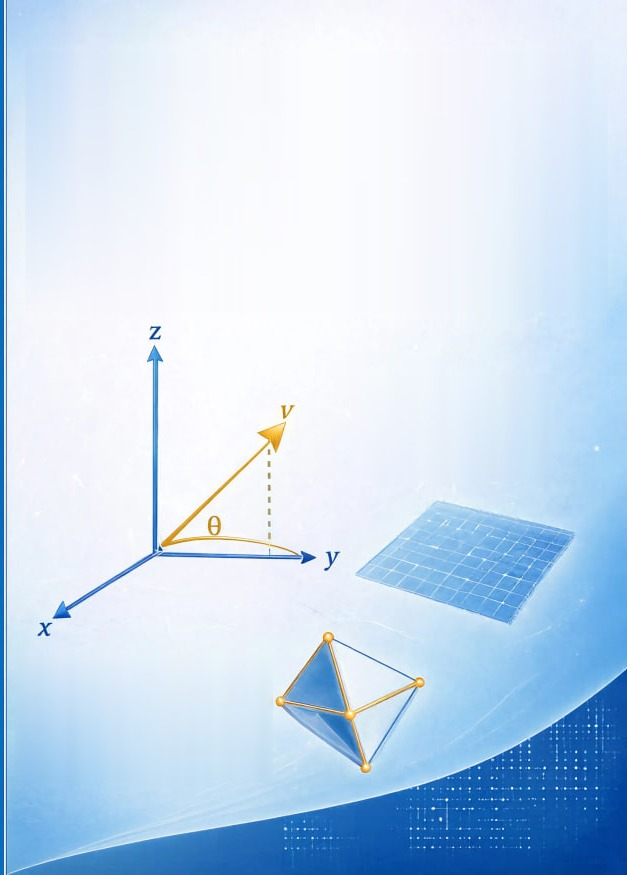
\includegraphics[width=\paperwidth,height=\paperheight]{rasmlar/cover_en.jpg}}%
  \put(\LenToUnit{-1in-\hoffset-\oddsidemargin},%
       \LenToUnit{1in+\voffset+\topmargin+\headheight+\headsep-0.17\paperheight}){%
    \makebox[\paperwidth]{\parbox{0.82\paperwidth}{\centering
      \color[RGB]{25,75,155}\fontsize{34}{38}\selectfont\bfseries LINEAR\\ALGEBRA\par
      \vspace{4mm}{\color[RGB]{200,150,50}\rule{0.55\paperwidth}{0.8pt}}\par
      \vspace{3mm}\color[RGB]{30,45,80}\normalfont\Large Nodirjon I. Tolipov\par}}}%
\end{picture}%
\null
\clearpage

% ============================================================
% 2. TITLE PAGE (data from sozlamalar/kitob-malumotlari.tex)
% ============================================================
\begin{titlepage}
\thispagestyle{empty}
\centering
{\small\bfseries\Vazirlik\par}
\vspace{0.6cm}
{\normalsize\bfseries\Muassasa\par}
\vspace{2.5cm}
{\large\Muallif\par}
\vspace{1.2cm}
{\Huge\bfseries\KitobNomiKatta\par}
\vspace{0.8cm}
{\large\itshape\KitobTuri\par}
\vfill
{\normalsize\Shahar~–~\Yil\par}
\end{titlepage}
\clearpage
% !Mode:: "TeX:UTF-8"
% ============================================================
% IMPRINT PAGE: UDC/LBC, abstract, reviewers, ISBN
% ============================================================
\thispagestyle{empty}
\noindent UDC \UOK\\
LBC \KBK

\bigskip
\noindent\MuallifQisqa. \KitobNomi: \KitobTuri. – \Shahar, \Yil.

\bigskip
\noindent\small
% Abstract:
The study guide covers the 24 topics of the course “Linear Algebra”: matrices
and determinants, systems of linear equations, vectors and analytic
geometry, linear and Euclidean spaces, linear operators, quadratic forms
and iterative methods for linear systems. Each topic contains the necessary
theory, examples solved in full detail, applications in information
security and short computations in Python, Maple and Mathcad. More than
two thousand exercises for independent work are included, all with
answers. The guide is intended for university students of information
security, computer engineering and other engineering programmes.
\normalsize

\vfill
\noindent\textbf{Reviewers:}\\
\TaqrizchiBir\\
\TaqrizchiIkki

\bigskip
\noindent\small
% Recommendation for publication:
Recommended for publication by the Council of Fergana State Technical
University (minutes No.~\rule{0.8cm}{0.4pt} of \rule{1.2cm}{0.4pt}~\Yil).
\normalsize

\bigskip
\noindent ISBN \rule{3cm}{0.4pt} \hfill \copyright~\MuallifQisqa, \Yil
\clearpage

\tableofcontents
% !Mode:: "TeX:UTF-8"
% ============================================================
% INTRODUCTION
% ============================================================
\chapter*{Introduction}
\addcontentsline{toc}{chapter}{Introduction}
\markboth{INTRODUCTION}{INTRODUCTION}

Linear algebra is one of the most widely used branches of modern
mathematics. Matrices, determinants, systems of linear equations, vector
spaces, linear operators and quadratic forms are the working language of
engineering computation, computer graphics and machine learning, and they
are equally basic to \textbf{information security}. The same methods appear
in the classical Hill cipher and in modern lattice-based (post-quantum)
cryptography, in error-detecting and error-correcting codes, and in the
analysis of network traffic and the detection of anomalies.

This study guide accompanies the course “Linear Algebra” and covers the
24 topics of its syllabus. The topics are grouped into five chapters.
Chapter~1, \emph{Matrices and Determinants} (Sections 1.1–1.6), deals with
operations on matrices, determinants of the second, third and $n$-th order,
minors and cofactors, the rank of a matrix and the inverse matrix.
Chapter~2, \emph{Systems of Linear Algebraic Equations, Vectors and Lines in
the Plane} (Sections 2.1–2.6), presents Cramer’s rule, the matrix method and
the Gauss and Gauss–Jordan methods, then turns to vectors, their scalar,
vector and triple products, and the equations of a straight line in the
plane. Chapter~3, \emph{Lines and Planes in Space; Linear and Euclidean
Spaces} (Sections 3.1–3.5), studies lines and planes in space, bases and
subspaces of a linear space, the norm in a Euclidean space and the
construction of orthonormal bases. Chapter~4, \emph{Linear Operators}
(Sections 4.1–4.3), treats linear operators and their matrices, eigenvalues
and eigenvectors, and diagonalization. Chapter~5, \emph{Quadratic Forms,
Second-Order Curves and Iterative Methods} (Sections 5.1–5.4), reduces
quadratic forms and second-order curves to canonical form and closes with
two approximate methods for linear systems, simple (Jacobi) iteration and
the Gauss–Seidel method.

All sections are built in the same way. The main definitions and theorems
come first, followed by worked examples solved in full detail. A separate
subsection shows how the material of the section is used in
\textbf{information security}, so that the reader sees why an engineer in
this field needs it. Each section also contains short examples of the same
computations in Python, Maple and Mathcad. The section ends with a
\textbf{collection of exercises}; every exercise set has 30 variants, which
allows a teacher to give each student in a group an individual assignment,
and the sets are supplemented by applied problems. The answers to all
exercises are collected at the end of the book in “Answers to the
Exercises”, arranged by section and exercise set.

We recommend reading the theory and the worked examples carefully before
attempting the exercises, and comparing one’s own results with the answers
only after the work is done. Checking the computations on a computer, in
Python, MATLAB, Maple or Mathcad, is also useful.

The guide is written for students of information security, computer
engineering, software engineering and other engineering programmes at
universities, and for anyone who studies linear algebra independently.


% ------------------------------------------------------------
% MAIN MATTER (arabic page numbers)
% Put % at the start of a line to leave a chapter out temporarily.
% ------------------------------------------------------------
\mainmatter
\subfile{boblar/bob1}
\subfile{boblar/bob2}
\subfile{boblar/bob3}
\subfile{boblar/bob4}
\subfile{boblar/bob5}

% ------------------------------------------------------------
% BACK MATTER
% ------------------------------------------------------------
\backmatter
% !Mode:: "TeX:UTF-8"
% ============================================================
% CONCLUSION
% ============================================================
\chapter*{Conclusion}
\addcontentsline{toc}{chapter}{Conclusion}
\markboth{CONCLUSION}{CONCLUSION}

This study guide has presented the theory, worked examples and exercises
needed for the practical part of a course in linear algebra. The material
starts with matrices and determinants and proceeds through exact methods
for systems of linear equations (Cramer’s rule, the matrix method, the
Gauss and Gauss–Jordan methods) and approximate ones (simple iteration and
the Gauss–Seidel method), vector algebra, elements of analytic geometry,
linear and Euclidean spaces, linear operators, eigenvalues and
eigenvectors, and quadratic forms.

Every topic has been connected with its use in information security: the
Hill cipher, error-correcting codes, secret sharing schemes, linear
cryptanalysis, lattice-based cryptography, network analysis and anomaly
detection. These applications are meant to show students that linear
algebra is not only an abstract theory but a tool they will use directly in
their profession. The short Python, Maple and Mathcad examples show how the
same computations are carried out in practice, where matrices are large and
hand calculation is no longer an option.

The more than two thousand exercises, all supplied with answers, give
students ample material for independent work and allow teachers to prepare
individual assignments. The knowledge and skills acquired here form the
basis for subsequent courses such as discrete mathematics, probability
theory, numerical methods, cryptography and coding theory.

% !Mode:: "TeX:UTF-8"
% ============================================================
% ANSWERS TO THE EXERCISES
% (checked automatically: all answers were computed with SymPy)
% ============================================================
\chapter*{Answers to the Exercises}
\addcontentsline{toc}{chapter}{Answers to the Exercises}
\markboth{ANSWERS TO THE EXERCISES}{ANSWERS TO THE EXERCISES}

\small
The answers are arranged by section, exercise set and exercise number.
Inverse matrices are written with the common denominator taken outside
the matrix. Approximate values are rounded to four decimal places.

\section*{Chapter 1. Matrices and Determinants}
% !Mode:: "TeX:UTF-8"
\javobmashgulot{1}{The concept of a matrix}
\par\noindent\emph{Exercise set 1.}\nopagebreak
\begin{multicols}{2}\raggedright
\begin{enumerate}[label=\arabic*., leftmargin=*, itemsep=1pt]
\item $\left(\begin{smallmatrix}-13 & -51\\ 68 & 4\end{smallmatrix}\right)$
\item $\left(\begin{smallmatrix}-21 & -15\\ 10 & 9\end{smallmatrix}\right)$
\item $\left(\begin{smallmatrix}-15 & -2\\ 4 & -8\end{smallmatrix}\right)$
\item $\left(\begin{smallmatrix}-21 & -2\\ -8 & -5\end{smallmatrix}\right)$
\item $\left(\begin{smallmatrix}28 & 32\\ -24 & 44\end{smallmatrix}\right)$
\item $\left(\begin{smallmatrix}-3 & -1\\ 3 & -8\end{smallmatrix}\right)$
\item $\left(\begin{smallmatrix}-13 & -12\\ -6 & -7\end{smallmatrix}\right)$
\item $\left(\begin{smallmatrix}-2 & -8\\ -16 & -10\end{smallmatrix}\right)$
\item $\left(\begin{smallmatrix}8 & 21\\ 0 & -20\end{smallmatrix}\right)$
\item $\left(\begin{smallmatrix}21 & 22\\ -33 & 10\end{smallmatrix}\right)$
\item $\left(\begin{smallmatrix}2 & -3\\ -9 & -4\end{smallmatrix}\right)$
\item $\left(\begin{smallmatrix}-15 & 6\\ 8 & -9\end{smallmatrix}\right)$
\item $\left(\begin{smallmatrix}14 & -15\\ 60 & -1\end{smallmatrix}\right)$
\item $\left(\begin{smallmatrix}-19 & 12\\ 3 & -10\end{smallmatrix}\right)$
\item $\left(\begin{smallmatrix}21 & 6\\ -6 & 13\end{smallmatrix}\right)$
\item $\left(\begin{smallmatrix}-53 & 24\\ 48 & -29\end{smallmatrix}\right)$
\item $\left(\begin{smallmatrix}-18 & -26\\ -39 & -31\end{smallmatrix}\right)$
\item $\left(\begin{smallmatrix}-26 & 30\\ -20 & 14\end{smallmatrix}\right)$
\item $\left(\begin{smallmatrix}-3 & 0\\ 0 & -3\end{smallmatrix}\right)$
\item $\left(\begin{smallmatrix}-3 & -8\\ -8 & 5\end{smallmatrix}\right)$
\item $\left(\begin{smallmatrix}10 & -20\\ -5 & -15\end{smallmatrix}\right)$
\item $\left(\begin{smallmatrix}-26 & 26\\ -104 & -26\end{smallmatrix}\right)$
\item $\left(\begin{smallmatrix}-27 & -4\\ -3 & -29\end{smallmatrix}\right)$
\item $\left(\begin{smallmatrix}-5 & -7\\ -7 & -26\end{smallmatrix}\right)$
\item $\left(\begin{smallmatrix}-5 & -6\\ -6 & 1\end{smallmatrix}\right)$
\item $\left(\begin{smallmatrix}-3 & 0\\ 9 & -12\end{smallmatrix}\right)$
\item $\left(\begin{smallmatrix}7 & -3\\ 6 & 7\end{smallmatrix}\right)$
\item $\left(\begin{smallmatrix}-15 & 28\\ 7 & -29\end{smallmatrix}\right)$
\item $\left(\begin{smallmatrix}-2 & -1\\ -1 & 1\end{smallmatrix}\right)$
\item $\left(\begin{smallmatrix}-22 & 0\\ 0 & -22\end{smallmatrix}\right)$
\end{enumerate}
\end{multicols}
\par\noindent\emph{Exercise set 2.}\nopagebreak
\begin{enumerate}[label=\arabic*., leftmargin=*, itemsep=1pt]
\item $A+A^T=\left(\begin{smallmatrix}-4 & 0 & 11\\ 0 & -2 & 6\\ 11 & 6 & -2\end{smallmatrix}\right)$
\item $A+A^T=\left(\begin{smallmatrix}-10 & -8\\ -8 & -6\end{smallmatrix}\right)$
\item $A+A^T=\left(\begin{smallmatrix}-6 & 0 & -9\\ 0 & 6 & 4\\ -9 & 4 & 8\end{smallmatrix}\right)$
\item $A+A^T=\left(\begin{smallmatrix}12 & -1\\ -1 & 8\end{smallmatrix}\right)$
\item $A+A^T=\left(\begin{smallmatrix}0 & 11\\ 11 & 12\end{smallmatrix}\right)$
\item $A+A^T=\left(\begin{smallmatrix}2 & -4\\ -4 & 12\end{smallmatrix}\right)$
\item $A+A^T=\left(\begin{smallmatrix}-10 & 11\\ 11 & 0\end{smallmatrix}\right)$
\item $A+A^T=\left(\begin{smallmatrix}0 & 10 & -9\\ 10 & -8 & -10\\ -9 & -10 & -8\end{smallmatrix}\right)$
\item $A+A^T=\left(\begin{smallmatrix}2 & 2 & 5\\ 2 & 6 & 7\\ 5 & 7 & -2\end{smallmatrix}\right)$
\item $A+A^T=\left(\begin{smallmatrix}4 & -2\\ -2 & -12\end{smallmatrix}\right)$
\item $A+A^T=\left(\begin{smallmatrix}12 & 9\\ 9 & -10\end{smallmatrix}\right)$
\item $A+A^T=\left(\begin{smallmatrix}10 & -7 & -2\\ -7 & -6 & -9\\ -2 & -9 & -4\end{smallmatrix}\right)$
\item $A+A^T=\left(\begin{smallmatrix}-6 & 5 & 3\\ 5 & -4 & -2\\ 3 & -2 & -12\end{smallmatrix}\right)$
\item $A+A^T=\left(\begin{smallmatrix}2 & 7\\ 7 & 4\end{smallmatrix}\right)$
\item $A+A^T=\left(\begin{smallmatrix}4 & -8 & -4\\ -8 & 4 & 3\\ -4 & 3 & 12\end{smallmatrix}\right)$
\item $A+A^T=\left(\begin{smallmatrix}6 & 0\\ 0 & 12\end{smallmatrix}\right)$
\item $A+A^T=\left(\begin{smallmatrix}-8 & -3\\ -3 & 6\end{smallmatrix}\right)$
\item $A+A^T=\left(\begin{smallmatrix}4 & -7\\ -7 & 8\end{smallmatrix}\right)$
\item $A+A^T=\left(\begin{smallmatrix}4 & 8 & 3\\ 8 & 12 & -11\\ 3 & -11 & -6\end{smallmatrix}\right)$
\item $A+A^T=\left(\begin{smallmatrix}-4 & 0\\ 0 & -10\end{smallmatrix}\right)$
\item $A+A^T=\left(\begin{smallmatrix}2 & 8 & -7\\ 8 & -10 & 4\\ -7 & 4 & 4\end{smallmatrix}\right)$
\item $A+A^T=\left(\begin{smallmatrix}4 & -5 & 7\\ -5 & 2 & 8\\ 7 & 8 & 2\end{smallmatrix}\right)$
\item $A+A^T=\left(\begin{smallmatrix}-6 & 3 & 3\\ 3 & 4 & -7\\ 3 & -7 & 0\end{smallmatrix}\right)$
\item $A+A^T=\left(\begin{smallmatrix}0 & 0\\ 0 & -10\end{smallmatrix}\right)$
\item $A+A^T=\left(\begin{smallmatrix}0 & -8\\ -8 & 8\end{smallmatrix}\right)$
\item $A+A^T=\left(\begin{smallmatrix}12 & 1\\ 1 & -8\end{smallmatrix}\right)$
\item $A+A^T=\left(\begin{smallmatrix}-8 & -6\\ -6 & 2\end{smallmatrix}\right)$
\item $A+A^T=\left(\begin{smallmatrix}10 & -5\\ -5 & 2\end{smallmatrix}\right)$
\item $A+A^T=\left(\begin{smallmatrix}8 & -7\\ -7 & 10\end{smallmatrix}\right)$
\item $A+A^T=\left(\begin{smallmatrix}4 & 0 & -2\\ 0 & -6 & -6\\ -2 & -6 & 10\end{smallmatrix}\right)$
\end{enumerate}
\par\noindent\emph{Exercise set 3.}\nopagebreak
\begin{multicols}{4}\raggedright
\begin{enumerate}[label=\arabic*., leftmargin=*, itemsep=1pt]
\item $Z=-4 X+2 Y$
\item $Z=-3 X- Y$
\item $Z=-2 X+2 Y$
\item $Z=3 X+ Y$
\item $Z=-4 X-3 Y$
\item $Z=-3 X+3 Y$
\item $Z=-2 X-4 Y$
\item $Z=-2 X- Y$
\item $Z=3 X+4 Y$
\item $Z=-4 X-4 Y$
\item $Z=- X+3 Y$
\item $Z=4 X+2 Y$
\item $Z=-2 X+2 Y$
\item $Z=2 X-2 Y$
\item $Z=- X-4 Y$
\item $Z= X+ Y$
\item $Z= X-2 Y$
\item $Z=4 X- Y$
\item $Z=-2 X+2 Y$
\item $Z=- X-3 Y$
\item $Z= X+3 Y$
\item $Z=4 X+2 Y$
\item $Z=- X-3 Y$
\item $Z=2 X+3 Y$
\item $Z=- X+3 Y$
\item $Z=-3 X+4 Y$
\item $Z=- X- Y$
\item $Z=-4 X- Y$
\item $Z=-2 X-4 Y$
\item $Z=- X+3 Y$
\end{enumerate}
\end{multicols}
\par\noindent\emph{Exercise set 4.}\nopagebreak
\begin{multicols}{2}\raggedright
\begin{enumerate}[label=\arabic*., leftmargin=*, itemsep=1pt]
\item $a=9,\ b=9$
\item $a=3,\ b=9$
\item $a=9,\ b=6$
\item $a=3,\ b=4$
\item $a=6,\ b=3$
\item $a=8,\ b=2$
\item $a=9,\ b=8$
\item $a=8,\ b=7$
\item $a=7,\ b=8$
\item $a=6,\ b=7$
\item $a=3,\ b=7$
\item $a=3,\ b=2$
\item $a=5,\ b=6$
\item $a=7,\ b=8$
\item $a=5,\ b=3$
\item $a=4,\ b=6$
\item $a=4,\ b=9$
\item $a=6,\ b=6$
\item $a=9,\ b=8$
\item $a=3,\ b=5$
\item $a=9,\ b=7$
\item $a=5,\ b=5$
\item $a=3,\ b=7$
\item $a=5,\ b=2$
\item $a=5,\ b=8$
\item $a=6,\ b=7$
\item $a=5,\ b=3$
\item $a=9,\ b=8$
\item $a=8,\ b=9$
\item $a=8,\ b=9$
\end{enumerate}
\end{multicols}
\par\noindent\emph{Exercise set 5.}\nopagebreak
\begin{enumerate}[label=\arabic*., leftmargin=*, itemsep=1pt]
\item 12 sizes: $1\times72,\ 2\times36,\ 3\times24,\ 4\times18,\ 6\times12,\ 8\times9,\ 9\times8,\ 12\times6,\ 18\times4,\ 24\times3,\ 36\times2,\ 72\times1$
\item 9 sizes: $1\times36,\ 2\times18,\ 3\times12,\ 4\times9,\ 6\times6,\ 9\times4,\ 12\times3,\ 18\times2,\ 36\times1$
\item 8 sizes: $1\times30,\ 2\times15,\ 3\times10,\ 5\times6,\ 6\times5,\ 10\times3,\ 15\times2,\ 30\times1$
\item 8 sizes: $1\times42,\ 2\times21,\ 3\times14,\ 6\times7,\ 7\times6,\ 14\times3,\ 21\times2,\ 42\times1$
\item 7 sizes: $1\times64,\ 2\times32,\ 4\times16,\ 8\times8,\ 16\times4,\ 32\times2,\ 64\times1$
\item 6 sizes: $1\times28,\ 2\times14,\ 4\times7,\ 7\times4,\ 14\times2,\ 28\times1$
\item 8 sizes: $1\times88,\ 2\times44,\ 4\times22,\ 8\times11,\ 11\times8,\ 22\times4,\ 44\times2,\ 88\times1$
\item 6 sizes: $1\times44,\ 2\times22,\ 4\times11,\ 11\times4,\ 22\times2,\ 44\times1$
\item 10 sizes: $1\times48,\ 2\times24,\ 3\times16,\ 4\times12,\ 6\times8,\ 8\times6,\ 12\times4,\ 16\times3,\ 24\times2,\ 48\times1$
\item 6 sizes: $1\times75,\ 3\times25,\ 5\times15,\ 15\times5,\ 25\times3,\ 75\times1$
\item 8 sizes: $1\times54,\ 2\times27,\ 3\times18,\ 6\times9,\ 9\times6,\ 18\times3,\ 27\times2,\ 54\times1$
\item 8 sizes: $1\times40,\ 2\times20,\ 4\times10,\ 5\times8,\ 8\times5,\ 10\times4,\ 20\times2,\ 40\times1$
\item 8 sizes: $1\times66,\ 2\times33,\ 3\times22,\ 6\times11,\ 11\times6,\ 22\times3,\ 33\times2,\ 66\times1$
\item 6 sizes: $1\times63,\ 3\times21,\ 7\times9,\ 9\times7,\ 21\times3,\ 63\times1$
\item 6 sizes: $1\times45,\ 3\times15,\ 5\times9,\ 9\times5,\ 15\times3,\ 45\times1$
\item 6 sizes: $1\times12,\ 2\times6,\ 3\times4,\ 4\times3,\ 6\times2,\ 12\times1$
\item 5 sizes: $1\times16,\ 2\times8,\ 4\times4,\ 8\times2,\ 16\times1$
\item 12 sizes: $1\times60,\ 2\times30,\ 3\times20,\ 4\times15,\ 5\times12,\ 6\times10,\ 10\times6,\ 12\times5,\ 15\times4,\ 20\times3,\ 30\times2,\ 60\times1$
\item 6 sizes: $1\times18,\ 2\times9,\ 3\times6,\ 6\times3,\ 9\times2,\ 18\times1$
\item 12 sizes: $1\times96,\ 2\times48,\ 3\times32,\ 4\times24,\ 6\times16,\ 8\times12,\ 12\times8,\ 16\times6,\ 24\times4,\ 32\times3,\ 48\times2,\ 96\times1$
\item 12 sizes: $1\times84,\ 2\times42,\ 3\times28,\ 4\times21,\ 6\times14,\ 7\times12,\ 12\times7,\ 14\times6,\ 21\times4,\ 28\times3,\ 42\times2,\ 84\times1$
\item 8 sizes: $1\times70,\ 2\times35,\ 5\times14,\ 7\times10,\ 10\times7,\ 14\times5,\ 35\times2,\ 70\times1$
\item 8 sizes: $1\times56,\ 2\times28,\ 4\times14,\ 7\times8,\ 8\times7,\ 14\times4,\ 28\times2,\ 56\times1$
\item 10 sizes: $1\times80,\ 2\times40,\ 4\times20,\ 5\times16,\ 8\times10,\ 10\times8,\ 16\times5,\ 20\times4,\ 40\times2,\ 80\times1$
\item 8 sizes: $1\times24,\ 2\times12,\ 3\times8,\ 4\times6,\ 6\times4,\ 8\times3,\ 12\times2,\ 24\times1$
\item 12 sizes: $1\times90,\ 2\times45,\ 3\times30,\ 5\times18,\ 6\times15,\ 9\times10,\ 10\times9,\ 15\times6,\ 18\times5,\ 30\times3,\ 45\times2,\ 90\times1$
\item 6 sizes: $1\times20,\ 2\times10,\ 4\times5,\ 5\times4,\ 10\times2,\ 20\times1$
\item 5 sizes: $1\times81,\ 3\times27,\ 9\times9,\ 27\times3,\ 81\times1$
\item 6 sizes: $1\times32,\ 2\times16,\ 4\times8,\ 8\times4,\ 16\times2,\ 32\times1$
\item 6 sizes: $1\times50,\ 2\times25,\ 5\times10,\ 10\times5,\ 25\times2,\ 50\times1$
\end{enumerate}
\par\noindent\emph{Exercise set 6.}\nopagebreak
\begin{enumerate}[label=\arabic*., leftmargin=*, itemsep=1pt]
\item $\left(\begin{smallmatrix}-1 & 9\\ 3 & -2\\ 0 & -4\end{smallmatrix}\right)$
\item $\left(\begin{smallmatrix}1 & -6 & 8\\ 1 & -5 & 3\\ 6 & -3 & -12\end{smallmatrix}\right)$
\item $\left(\begin{smallmatrix}1 & -1 & -15\\ -4 & 9 & -17\end{smallmatrix}\right)$
\item $\left(\begin{smallmatrix}-2 & -10 & 14\\ 4 & 14 & -8\end{smallmatrix}\right)$
\item $\left(\begin{smallmatrix}-9 & 13 & -2\\ 19 & 3 & 13\\ 2 & 15 & -4\end{smallmatrix}\right)$
\item $\left(\begin{smallmatrix}7 & -9\\ -13 & -6\\ -4 & 4\end{smallmatrix}\right)$
\item $\left(\begin{smallmatrix}-7 & -6\\ -5 & -2\end{smallmatrix}\right)$
\item $\left(\begin{smallmatrix}2 & 20\\ 16 & -8\\ 8 & 4\end{smallmatrix}\right)$
\item $\left(\begin{smallmatrix}1 & -4 & -6\\ -1 & -9 & 6\end{smallmatrix}\right)$
\item $\left(\begin{smallmatrix}3 & 11\\ -7 & -14\\ 12 & 16\end{smallmatrix}\right)$
\item $\left(\begin{smallmatrix}-10 & -15 & 19\\ -11 & -6 & 9\\ 2 & 9 & 31\end{smallmatrix}\right)$
\item $\left(\begin{smallmatrix}17 & -12 & -13\\ -7 & -8 & 19\end{smallmatrix}\right)$
\item $\left(\begin{smallmatrix}6 & -9\\ 6 & 2\end{smallmatrix}\right)$
\item $\left(\begin{smallmatrix}-4 & 6 & 5\\ 6 & -1 & -1\end{smallmatrix}\right)$
\item $\left(\begin{smallmatrix}10 & -13 & -2\\ 2 & -21 & -15\\ 20 & -26 & 16\end{smallmatrix}\right)$
\item $\left(\begin{smallmatrix}15 & 14\\ 10 & 2\end{smallmatrix}\right)$
\item $\left(\begin{smallmatrix}-15 & -10 & 10\\ 11 & 5 & -14\end{smallmatrix}\right)$
\item $\left(\begin{smallmatrix}-7 & -10 & 8\\ 7 & -9 & -12\end{smallmatrix}\right)$
\item $\left(\begin{smallmatrix}2 & 20\\ 6 & -24\\ 0 & -26\end{smallmatrix}\right)$
\item $\left(\begin{smallmatrix}-21 & -11 & 15\\ -15 & 11 & -3\end{smallmatrix}\right)$
\item $\left(\begin{smallmatrix}-4 & 16 & -2\\ -2 & 12 & -4\\ -10 & 4 & 6\end{smallmatrix}\right)$
\item $\left(\begin{smallmatrix}-1 & -13\\ 13 & 21\end{smallmatrix}\right)$
\item $\left(\begin{smallmatrix}22 & 16 & -2\\ -2 & 2 & 10\end{smallmatrix}\right)$
\item $\left(\begin{smallmatrix}-4 & 28 & -14\\ -12 & -8 & 20\\ -22 & 20 & -24\end{smallmatrix}\right)$
\item $\left(\begin{smallmatrix}-13 & 6 & 22\\ -1 & 16 & 6\end{smallmatrix}\right)$
\item $\left(\begin{smallmatrix}12 & 30 & -3\\ 21 & 12 & 3\\ 3 & -21 & -12\end{smallmatrix}\right)$
\item $\left(\begin{smallmatrix}-18 & -24 & -15\\ 9 & -3 & -3\end{smallmatrix}\right)$
\item $\left(\begin{smallmatrix}-20 & 26\\ -20 & -26\end{smallmatrix}\right)$
\item $\left(\begin{smallmatrix}-9 & -2 & 10\\ -14 & 2 & 5\end{smallmatrix}\right)$
\item $\left(\begin{smallmatrix}-2 & -1\\ 2 & 2\\ 5 & 0\end{smallmatrix}\right)$
\end{enumerate}
\par\noindent\emph{Exercise set 7.}\nopagebreak
\begin{enumerate}[label=\arabic*., leftmargin=*, itemsep=1pt]
\item $c=\left(\begin{smallmatrix}0\\25\end{smallmatrix}\right)$ ($Kp=(78;103)^T$)
\item $c=\left(\begin{smallmatrix}16\\3\end{smallmatrix}\right)$
\item $c=\left(\begin{smallmatrix}0\\19\end{smallmatrix}\right)$
\item $c=\left(\begin{smallmatrix}3\\15\end{smallmatrix}\right)$
\item $\det K=-2$, $\gcd(-2,26)=2$; since $\gcd(\det K,26)\ne1$, $K$ is not invertible modulo $26$ and cannot serve as a key
\item $\det K=0$; $K$ is singular (has no inverse), so it cannot serve as a key
\item $c=(1;0;1;1;0;1;0)$
\item $s=(0;0;1)^T\ne0$; the word contains an error. The syndrome equals the 4th column of $H$, so the 4th bit is wrong; the corrected word is $(1;0;1;0;1;0;1)$
\item $A^2=\left(\begin{smallmatrix}2&0&0&2&1\\0&2&2&0&1\\0&2&3&1&1\\2&0&1&3&1\\1&1&1&1&2\end{smallmatrix}\right)$; the most connected nodes are $S_3$ and $S_4$ (degree 3, the diagonal entries of $A^2$)
\item $K^2-3K+E=O$, hence $K(3E-K)=E$ and $K^{-1}=3E-K=\left(\begin{smallmatrix}1&-1\\-1&2\end{smallmatrix}\right)$
\end{enumerate}

% !Mode:: "TeX:UTF-8"
\javobmashgulot{2}{The concept of a determinant. Determinants of the second and third order}
\par\noindent\emph{Exercise set 1.}\nopagebreak
\begin{multicols}{5}\raggedright
\begin{enumerate}[label=\arabic*., leftmargin=*, itemsep=1pt]
\item $22$
\item $-11$
\item $20$
\item $42$
\item $32$
\item $16$
\item $35$
\item $-14$
\item $26$
\item $18$
\item $58$
\item $3$
\item $27$
\item $18$
\item $13$
\item $0$
\item $-41$
\item $84$
\item $28$
\item $-3$
\item $19$
\item $-43$
\item $-26$
\item $31$
\item $42$
\item $7$
\item $-37$
\item $35$
\item $-46$
\item $1$
\end{enumerate}
\end{multicols}
\par\noindent\emph{Exercise set 2.}\nopagebreak
\begin{multicols}{5}\raggedright
\begin{enumerate}[label=\arabic*., leftmargin=*, itemsep=1pt]
\item $6$
\item $83$
\item $17$
\item $38$
\item $65$
\item $90$
\item $-89$
\item $77$
\item $89$
\item $75$
\item $-32$
\item $-47$
\item $22$
\item $17$
\item $-52$
\item $-17$
\item $16$
\item $22$
\item $117$
\item $-129$
\item $39$
\item $51$
\item $71$
\item $7$
\item $20$
\item $49$
\item $87$
\item $24$
\item $66$
\item $-55$
\end{enumerate}
\end{multicols}
\par\noindent\emph{Exercise set 3.}\nopagebreak
\begin{multicols}{5}\raggedright
\begin{enumerate}[label=\arabic*., leftmargin=*, itemsep=1pt]
\item $-77$
\item $23$
\item $100$
\item $51$
\item $90$
\item $106$
\item $102$
\item $50$
\item $-79$
\item $13$
\item $-75$
\item $-70$
\item $83$
\item $93$
\item $5$
\item $-18$
\item $-31$
\item $63$
\item $73$
\item $-86$
\item $9$
\item $1$
\item $-36$
\item $24$
\item $63$
\item $27$
\item $-20$
\item $42$
\item $20$
\item $66$
\end{enumerate}
\end{multicols}
\par\noindent\emph{Exercise set 4.}\nopagebreak
\begin{multicols}{5}\raggedright
\begin{enumerate}[label=\arabic*., leftmargin=*, itemsep=1pt]
\item $0$
\item $0$
\item $-12$
\item $0$
\item $0$
\item $0$
\item $0$
\item $210$
\item $0$
\item $0$
\item $-15$
\item $0$
\item $0$
\item $0$
\item $0$
\item $0$
\item $0$
\item $0$
\item $-21$
\item $0$
\item $140$
\item $-42$
\item $0$
\item $0$
\item $-5$
\item $0$
\item $0$
\item $0$
\item $0$
\item $396$
\end{enumerate}
\end{multicols}
\par\noindent\emph{Exercise set 5.}\nopagebreak
\begin{multicols}{2}\raggedright
\begin{enumerate}[label=\arabic*., leftmargin=*, itemsep=1pt]
\item $\det K=11,\ \gcd(11,26)=1$ – admissible
\item $\det K=0,\ \gcd(0,26)=26$ – not admissible
\item $\det K=1,\ \gcd(1,26)=1$ – admissible
\item $\det K=19,\ \gcd(19,26)=1$ – admissible
\item $\det K=43,\ \gcd(43,26)=1$ – admissible
\item $\det K=0,\ \gcd(0,26)=26$ – not admissible
\item $\det K=-1,\ \gcd(-1,26)=1$ – admissible
\item $\det K=19,\ \gcd(19,26)=1$ – admissible
\item $\det K=51,\ \gcd(51,26)=1$ – admissible
\item $\det K=1,\ \gcd(1,26)=1$ – admissible
\item $\det K=89,\ \gcd(89,26)=1$ – admissible
\item $\det K=-2,\ \gcd(-2,26)=2$ – not admissible
\item $\det K=9,\ \gcd(9,26)=1$ – admissible
\item $\det K=-11,\ \gcd(-11,26)=1$ – admissible
\item $\det K=1,\ \gcd(1,26)=1$ – admissible
\item $\det K=2,\ \gcd(2,26)=2$ – not admissible
\item $\det K=24,\ \gcd(24,26)=2$ – not admissible
\item $\det K=31,\ \gcd(31,26)=1$ – admissible
\item $\det K=0,\ \gcd(0,26)=26$ – not admissible
\item $\det K=172,\ \gcd(172,26)=2$ – not admissible
\item $\det K=1,\ \gcd(1,26)=1$ – admissible
\item $\det K=26,\ \gcd(26,26)=26$ – not admissible
\item $\det K=17,\ \gcd(17,26)=1$ – admissible
\item $\det K=22,\ \gcd(22,26)=2$ – not admissible
\item $\det K=1,\ \gcd(1,26)=1$ – admissible
\item $\det K=-3,\ \gcd(-3,26)=1$ – admissible
\item $\det K=1,\ \gcd(1,26)=1$ – admissible
\item $\det K=-1,\ \gcd(-1,26)=1$ – admissible
\item $\det K=-29,\ \gcd(-29,26)=1$ – admissible
\item $\det K=53,\ \gcd(53,26)=1$ – admissible
\end{enumerate}
\end{multicols}

% !Mode:: "TeX:UTF-8"
\javobmashgulot{3}{Minors and cofactors. Evaluation of determinants of order \texorpdfstring{$n$}{n}}
\par\noindent\emph{Exercise set 1.}\nopagebreak
\begin{multicols}{2}\raggedright
\begin{enumerate}[label=\arabic*., leftmargin=*, itemsep=1pt]
\item $M_{11}=22,\ A_{11}=22;\,M_{23}=7,\ A_{23}=-7$
\item $M_{12}=-11,\ A_{12}=11;\,M_{31}=-1,\ A_{31}=-1$
\item $M_{22}=11,\ A_{22}=11;\,M_{13}=-2,\ A_{13}=-2$
\item $M_{32}=-20,\ A_{32}=20;\,M_{11}=33,\ A_{11}=33$
\item $M_{21}=-4,\ A_{21}=4;\,M_{33}=-6,\ A_{33}=-6$
\item $M_{13}=-6,\ A_{13}=-6;\,M_{22}=-8,\ A_{22}=-8$
\item $M_{31}=15,\ A_{31}=15;\,M_{12}=-7,\ A_{12}=7$
\item $M_{23}=-7,\ A_{23}=7;\,M_{11}=5,\ A_{11}=5$
\item $M_{32}=-12,\ A_{32}=12;\,M_{21}=-4,\ A_{21}=4$
\item $M_{11}=23,\ A_{11}=23;\,M_{33}=24,\ A_{33}=24$
\item $M_{12}=18,\ A_{12}=-18;\,M_{31}=-12,\ A_{31}=-12$
\item $M_{22}=-9,\ A_{22}=-9;\,M_{13}=-10,\ A_{13}=-10$
\item $M_{21}=4,\ A_{21}=-4;\,M_{32}=2,\ A_{32}=-2$
\item $M_{13}=6,\ A_{13}=6;\,M_{23}=-4,\ A_{23}=4$
\item $M_{11}=-18,\ A_{11}=-18;\,M_{32}=-26,\ A_{32}=26$
\item $M_{31}=10,\ A_{31}=10;\,M_{12}=-8,\ A_{12}=8$
\item $M_{22}=19,\ A_{22}=19;\,M_{33}=3,\ A_{33}=3$
\item $M_{13}=2,\ A_{13}=2;\,M_{21}=-4,\ A_{21}=4$
\item $M_{23}=-11,\ A_{23}=11;\,M_{11}=12,\ A_{11}=12$
\item $M_{32}=-12,\ A_{32}=12;\,M_{12}=3,\ A_{12}=-3$
\item $M_{11}=6,\ A_{11}=6;\,M_{23}=-10,\ A_{23}=10$
\item $M_{21}=-4,\ A_{21}=4;\,M_{33}=12,\ A_{33}=12$
\item $M_{31}=22,\ A_{31}=22;\,M_{22}=-20,\ A_{22}=-20$
\item $M_{12}=17,\ A_{12}=-17;\,M_{33}=20,\ A_{33}=20$
\item $M_{13}=4,\ A_{13}=4;\,M_{21}=4,\ A_{21}=-4$
\item $M_{22}=5,\ A_{22}=5;\,M_{31}=8,\ A_{31}=8$
\item $M_{32}=-6,\ A_{32}=6;\,M_{11}=-8,\ A_{11}=-8$
\item $M_{23}=-9,\ A_{23}=9;\,M_{12}=-21,\ A_{12}=21$
\item $M_{11}=-6,\ A_{11}=-6;\,M_{13}=4,\ A_{13}=4$
\item $M_{21}=4,\ A_{21}=-4;\,M_{32}=8,\ A_{32}=-8$
\end{enumerate}
\end{multicols}
\par\noindent\emph{Exercise set 2.}\nopagebreak
\begin{multicols}{5}\raggedright
\begin{enumerate}[label=\arabic*., leftmargin=*, itemsep=1pt]
\item $12$
\item $-79$
\item $24$
\item $-62$
\item $38$
\item $-36$
\item $66$
\item $-62$
\item $46$
\item $-49$
\item $70$
\item $62$
\item $-46$
\item $-54$
\item $-58$
\item $80$
\item $-64$
\item $-58$
\item $-30$
\item $-64$
\item $32$
\item $-62$
\item $85$
\item $62$
\item $53$
\item $56$
\item $-68$
\item $-39$
\item $14$
\item $32$
\end{enumerate}
\end{multicols}
\par\noindent\emph{Exercise set 3.}\nopagebreak
\begin{multicols}{5}\raggedright
\begin{enumerate}[label=\arabic*., leftmargin=*, itemsep=1pt]
\item $-10$
\item $-65$
\item $21$
\item $-8$
\item $-9$
\item $-134$
\item $92$
\item $114$
\item $110$
\item $83$
\item $1$
\item $212$
\item $-198$
\item $35$
\item $-160$
\item $-18$
\item $-52$
\item $28$
\item $-56$
\item $6$
\item $152$
\item $49$
\item $23$
\item $63$
\item $154$
\item $140$
\item $110$
\item $91$
\item $17$
\item $0$
\end{enumerate}
\end{multicols}
\par\noindent\emph{Exercise set 4.}\nopagebreak
\begin{multicols}{5}\raggedright
\begin{enumerate}[label=\arabic*., leftmargin=*, itemsep=1pt]
\item $79$ and $0$
\item $-70$ and $0$
\item $-60$ and $0$
\item $-90$ and $0$
\item $-54$ and $0$
\item $60$ and $0$
\item $-38$ and $0$
\item $-1$ and $0$
\item $50$ and $0$
\item $60$ and $0$
\item $7$ and $0$
\item $35$ and $0$
\item $64$ and $0$
\item $-41$ and $0$
\item $46$ and $0$
\item $75$ and $0$
\item $10$ and $0$
\item $48$ and $0$
\item $3$ and $0$
\item $45$ and $0$
\item $84$ and $0$
\item $23$ and $0$
\item $102$ and $0$
\item $49$ and $0$
\item $54$ and $0$
\item $21$ and $0$
\item $-40$ and $0$
\item $-5$ and $0$
\item $-55$ and $0$
\item $10$ and $0$
\end{enumerate}
\end{multicols}

% !Mode:: "TeX:UTF-8"
\javobmashgulot{4}{Computing the rank of a matrix. Singular and nonsingular matrices}
\par\noindent\emph{Exercise set 1.}\nopagebreak
\begin{multicols}{5}\raggedright
\begin{enumerate}[label=\arabic*., leftmargin=*, itemsep=1pt]
\item $\operatorname{rg}=2$
\item $\operatorname{rg}=2$
\item $\operatorname{rg}=1$
\item $\operatorname{rg}=2$
\item $\operatorname{rg}=2$
\item $\operatorname{rg}=3$
\item $\operatorname{rg}=1$
\item $\operatorname{rg}=2$
\item $\operatorname{rg}=1$
\item $\operatorname{rg}=2$
\item $\operatorname{rg}=1$
\item $\operatorname{rg}=2$
\item $\operatorname{rg}=2$
\item $\operatorname{rg}=2$
\item $\operatorname{rg}=3$
\item $\operatorname{rg}=1$
\item $\operatorname{rg}=2$
\item $\operatorname{rg}=3$
\item $\operatorname{rg}=1$
\item $\operatorname{rg}=2$
\item $\operatorname{rg}=1$
\item $\operatorname{rg}=2$
\item $\operatorname{rg}=2$
\item $\operatorname{rg}=1$
\item $\operatorname{rg}=2$
\item $\operatorname{rg}=2$
\item $\operatorname{rg}=1$
\item $\operatorname{rg}=3$
\item $\operatorname{rg}=1$
\item $\operatorname{rg}=2$
\end{enumerate}
\end{multicols}
\par\noindent\emph{Exercise set 2.}\nopagebreak
\begin{multicols}{5}\raggedright
\begin{enumerate}[label=\arabic*., leftmargin=*, itemsep=1pt]
\item $\operatorname{rg}=2$
\item $\operatorname{rg}=2$
\item $\operatorname{rg}=1$
\item $\operatorname{rg}=2$
\item $\operatorname{rg}=2$
\item $\operatorname{rg}=1$
\item $\operatorname{rg}=2$
\item $\operatorname{rg}=2$
\item $\operatorname{rg}=2$
\item $\operatorname{rg}=1$
\item $\operatorname{rg}=4$
\item $\operatorname{rg}=2$
\item $\operatorname{rg}=1$
\item $\operatorname{rg}=2$
\item $\operatorname{rg}=2$
\item $\operatorname{rg}=2$
\item $\operatorname{rg}=2$
\item $\operatorname{rg}=1$
\item $\operatorname{rg}=3$
\item $\operatorname{rg}=4$
\item $\operatorname{rg}=1$
\item $\operatorname{rg}=1$
\item $\operatorname{rg}=2$
\item $\operatorname{rg}=3$
\item $\operatorname{rg}=2$
\item $\operatorname{rg}=1$
\item $\operatorname{rg}=2$
\item $\operatorname{rg}=3$
\item $\operatorname{rg}=2$
\item $\operatorname{rg}=1$
\end{enumerate}
\end{multicols}
\par\noindent\emph{Exercise set 3.}\nopagebreak
\begin{multicols}{4}\raggedright
\begin{enumerate}[label=\arabic*., leftmargin=*, itemsep=1pt]
\item $\det=-2$, nonsingular
\item $\det=0$, singular
\item $\det=13$, nonsingular
\item $\det=0$, singular
\item $\det=-8$, nonsingular
\item $\det=0$, singular
\item $\det=0$, singular
\item $\det=0$, singular
\item $\det=0$, singular
\item $\det=60$, nonsingular
\item $\det=1$, nonsingular
\item $\det=0$, singular
\item $\det=0$, singular
\item $\det=1$, nonsingular
\item $\det=0$, singular
\item $\det=0$, singular
\item $\det=-30$, nonsingular
\item $\det=0$, singular
\item $\det=1$, nonsingular
\item $\det=0$, singular
\item $\det=0$, singular
\item $\det=-6$, nonsingular
\item $\det=0$, singular
\item $\det=0$, singular
\item $\det=0$, singular
\item $\det=4$, nonsingular
\item $\det=0$, singular
\item $\det=0$, singular
\item $\det=0$, singular
\item $\det=0$, singular
\end{enumerate}
\end{multicols}
\par\noindent\emph{Exercise set 4.}\nopagebreak
\begin{multicols}{2}\raggedright
\begin{enumerate}[label=\arabic*., leftmargin=*, itemsep=1pt]
\item $\operatorname{rg}A=\operatorname{rg}\bar A=2$; consistent (infinitely many solutions)
\item $\operatorname{rg}A=1,\ \operatorname{rg}\bar A=2$; inconsistent
\item $\operatorname{rg}A=\operatorname{rg}\bar A=2$; consistent (infinitely many solutions)
\item $\operatorname{rg}A=\operatorname{rg}\bar A=1$; consistent (infinitely many solutions)
\item $\operatorname{rg}A=\operatorname{rg}\bar A=2$; consistent (infinitely many solutions)
\item $\operatorname{rg}A=1,\ \operatorname{rg}\bar A=2$; inconsistent
\item $\operatorname{rg}A=\operatorname{rg}\bar A=2$; consistent (infinitely many solutions)
\item $\operatorname{rg}A=1,\ \operatorname{rg}\bar A=2$; inconsistent
\item $\operatorname{rg}A=\operatorname{rg}\bar A=2$; consistent (unique solution)
\item $\operatorname{rg}A=\operatorname{rg}\bar A=2$; consistent (infinitely many solutions)
\item $\operatorname{rg}A=\operatorname{rg}\bar A=1$; consistent (infinitely many solutions)
\item $\operatorname{rg}A=1,\ \operatorname{rg}\bar A=2$; inconsistent
\item $\operatorname{rg}A=\operatorname{rg}\bar A=1$; consistent (infinitely many solutions)
\item $\operatorname{rg}A=\operatorname{rg}\bar A=2$; consistent (infinitely many solutions)
\item $\operatorname{rg}A=\operatorname{rg}\bar A=1$; consistent (infinitely many solutions)
\item $\operatorname{rg}A=1,\ \operatorname{rg}\bar A=2$; inconsistent
\item $\operatorname{rg}A=\operatorname{rg}\bar A=3$; consistent (unique solution)
\item $\operatorname{rg}A=\operatorname{rg}\bar A=1$; consistent (infinitely many solutions)
\item $\operatorname{rg}A=\operatorname{rg}\bar A=2$; consistent (unique solution)
\item $\operatorname{rg}A=\operatorname{rg}\bar A=3$; consistent (infinitely many solutions)
\item $\operatorname{rg}A=\operatorname{rg}\bar A=1$; consistent (infinitely many solutions)
\item $\operatorname{rg}A=\operatorname{rg}\bar A=1$; consistent (infinitely many solutions)
\item $\operatorname{rg}A=\operatorname{rg}\bar A=2$; consistent (infinitely many solutions)
\item $\operatorname{rg}A=\operatorname{rg}\bar A=2$; consistent (unique solution)
\item $\operatorname{rg}A=\operatorname{rg}\bar A=1$; consistent (infinitely many solutions)
\item $\operatorname{rg}A=1,\ \operatorname{rg}\bar A=2$; inconsistent
\item $\operatorname{rg}A=2,\ \operatorname{rg}\bar A=3$; inconsistent
\item $\operatorname{rg}A=\operatorname{rg}\bar A=1$; consistent (infinitely many solutions)
\item $\operatorname{rg}A=1,\ \operatorname{rg}\bar A=2$; inconsistent
\item $\operatorname{rg}A=2,\ \operatorname{rg}\bar A=3$; inconsistent
\end{enumerate}
\end{multicols}

% !Mode:: "TeX:UTF-8"
\javobmashgulot{5}{The inverse matrix}
\par\noindent\emph{Exercise set 1.}\nopagebreak
\begin{multicols}{2}\raggedright
\begin{enumerate}[label=\arabic*., leftmargin=*, itemsep=1pt]
\item $\left(\begin{smallmatrix}2 & -1\\ -5 & 3\end{smallmatrix}\right)$
\item does not exist ($\det=0$)
\item $\left(\begin{smallmatrix}-5 & 2\\ 3 & -1\end{smallmatrix}\right)$
\item $\left(\begin{smallmatrix}1 & 3\\ 1 & 2\end{smallmatrix}\right)$
\item $\frac{1}{15}\left(\begin{smallmatrix}3 & 0\\ 0 & -5\end{smallmatrix}\right)$
\item does not exist ($\det=0$)
\item $\left(\begin{smallmatrix}5 & 3\\ 2 & 1\end{smallmatrix}\right)$
\item $\left(\begin{smallmatrix}1 & -2\\ -3 & 7\end{smallmatrix}\right)$
\item does not exist ($\det=0$)
\item $\left(\begin{smallmatrix}2 & 1\\ 1 & 1\end{smallmatrix}\right)$
\item $\left(\begin{smallmatrix}0 & 1\\ 1 & 0\end{smallmatrix}\right)$
\item does not exist ($\det=0$)
\item $\frac{1}{14}\left(\begin{smallmatrix}-3 & 1\\ 2 & 4\end{smallmatrix}\right)$
\item $\left(\begin{smallmatrix}1 & 0\\ 0 & 1\end{smallmatrix}\right)$
\item does not exist ($\det=0$)
\item $\frac{1}{17}\left(\begin{smallmatrix}3 & -2\\ 1 & 5\end{smallmatrix}\right)$
\item does not exist ($\det=0$)
\item $\left(\begin{smallmatrix}2 & -5\\ -3 & 8\end{smallmatrix}\right)$
\item $\left(\begin{smallmatrix}-7 & 4\\ 2 & -1\end{smallmatrix}\right)$
\item $\frac{1}{10}\left(\begin{smallmatrix}-5 & 0\\ 0 & -2\end{smallmatrix}\right)$
\item does not exist ($\det=0$)
\item $\frac{1}{13}\left(\begin{smallmatrix}1 & 1\\ -4 & 9\end{smallmatrix}\right)$
\item does not exist ($\det=0$)
\item $\left(\begin{smallmatrix}3 & -1\\ -5 & 2\end{smallmatrix}\right)$
\item $\left(\begin{smallmatrix}2 & -5\\ 1 & -3\end{smallmatrix}\right)$
\item $\frac{1}{6}\left(\begin{smallmatrix}0 & 2\\ -3 & 0\end{smallmatrix}\right)$
\item $\left(\begin{smallmatrix}11 & 4\\ -3 & -1\end{smallmatrix}\right)$
\item $\frac{1}{20}\left(\begin{smallmatrix}3 & -1\\ 2 & 6\end{smallmatrix}\right)$
\item does not exist ($\det=0$)
\item $\frac{1}{13}\left(\begin{smallmatrix}1 & 3\\ -2 & 7\end{smallmatrix}\right)$
\end{enumerate}
\end{multicols}
\par\noindent\emph{Exercise set 2.}\nopagebreak
\begin{enumerate}[label=\arabic*., leftmargin=*, itemsep=1pt]
\item $\left(\begin{smallmatrix}1 & -1 & 1\\ -38 & 41 & -34\\ 27 & -29 & 24\end{smallmatrix}\right)$
\item $\frac{1}{9}\left(\begin{smallmatrix}-1 & -2 & 5\\ 2 & 4 & -1\\ 6 & 3 & -3\end{smallmatrix}\right)$
\item $\frac{1}{73}\left(\begin{smallmatrix}26 & 5 & -2\\ 3 & 9 & 11\\ -5 & -15 & 6\end{smallmatrix}\right)$
\item $\frac{1}{41}\left(\begin{smallmatrix}2 & 11 & 1\\ 21 & 13 & -10\\ 8 & 3 & 4\end{smallmatrix}\right)$
\item $\frac{1}{10}\left(\begin{smallmatrix}4 & -8 & -6\\ 3 & 4 & 3\\ 1 & -2 & 1\end{smallmatrix}\right)$
\item $\frac{1}{43}\left(\begin{smallmatrix}5 & 1 & -10\\ -3 & 8 & 6\\ 10 & 2 & 23\end{smallmatrix}\right)$
\item $\frac{1}{16}\left(\begin{smallmatrix}8 & 4 & -4\\ 4 & 2 & 6\\ -6 & 1 & 3\end{smallmatrix}\right)$
\item $\frac{1}{8}\left(\begin{smallmatrix}2 & -9 & -3\\ 4 & -10 & -6\\ 2 & 3 & 1\end{smallmatrix}\right)$
\item $\frac{1}{16}\left(\begin{smallmatrix}4 & 2 & 14\\ 10 & 1 & 15\\ 8 & 4 & 12\end{smallmatrix}\right)$
\item $\frac{1}{54}\left(\begin{smallmatrix}10 & 4 & 2\\ -2 & 10 & 5\\ 4 & -20 & 17\end{smallmatrix}\right)$
\item $\frac{1}{20}\left(\begin{smallmatrix}15 & 5 & -10\\ -2 & 6 & 4\\ -3 & -1 & 6\end{smallmatrix}\right)$
\item $\frac{1}{48}\left(\begin{smallmatrix}-4 & 8 & 10\\ 2 & -4 & 7\\ 22 & 4 & 5\end{smallmatrix}\right)$
\item $\frac{1}{2}\left(\begin{smallmatrix}-20 & -11 & 12\\ 4 & 2 & -2\\ -10 & -5 & 6\end{smallmatrix}\right)$
\item $\frac{1}{49}\left(\begin{smallmatrix}10 & 6 & 3\\ -5 & -3 & -26\\ -3 & 8 & 4\end{smallmatrix}\right)$
\item $\frac{1}{53}\left(\begin{smallmatrix}6 & 9 & -2\\ -15 & 4 & 5\\ 8 & 12 & 15\end{smallmatrix}\right)$
\item $\frac{1}{61}\left(\begin{smallmatrix}17 & -5 & -1\\ 10 & 15 & 3\\ 6 & 9 & 14\end{smallmatrix}\right)$
\item $\frac{1}{39}\left(\begin{smallmatrix}5 & 11 & 2\\ -8 & -2 & -11\\ -20 & -5 & -8\end{smallmatrix}\right)$
\item $\frac{1}{17}\left(\begin{smallmatrix}4 & 1 & -3\\ 12 & 3 & 8\\ -9 & 2 & -6\end{smallmatrix}\right)$
\item $\frac{1}{26}\left(\begin{smallmatrix}-2 & -4 & -20\\ -7 & -1 & -5\\ -4 & -8 & -14\end{smallmatrix}\right)$
\item $\frac{1}{54}\left(\begin{smallmatrix}9 & 6 & 15\\ 12 & 8 & 2\\ 3 & 20 & 5\end{smallmatrix}\right)$
\item $\frac{1}{14}\left(\begin{smallmatrix}3 & 20 & 12\\ 1 & 2 & 4\\ 5 & 10 & 6\end{smallmatrix}\right)$
\item $\frac{1}{46}\left(\begin{smallmatrix}2 & 4 & 8\\ -20 & 6 & 12\\ -5 & -10 & 3\end{smallmatrix}\right)$
\item $\frac{1}{37}\left(\begin{smallmatrix}12 & 5 & 20\\ 9 & 13 & 15\\ -5 & 1 & 4\end{smallmatrix}\right)$
\item $\frac{1}{62}\left(\begin{smallmatrix}5 & 1 & -15\\ -2 & 12 & 6\\ 20 & 4 & 2\end{smallmatrix}\right)$
\item $\frac{1}{13}\left(\begin{smallmatrix}0 & 0 & 13\\ 5 & 1 & -20\\ 2 & 3 & -8\end{smallmatrix}\right)$
\item $\frac{1}{62}\left(\begin{smallmatrix}-20 & 2 & 8\\ 5 & 15 & -2\\ 1 & 3 & 12\end{smallmatrix}\right)$
\item $\frac{1}{27}\left(\begin{smallmatrix}12 & 20 & -3\\ 0 & 9 & 0\\ 3 & 5 & 6\end{smallmatrix}\right)$
\item $\frac{1}{2}\left(\begin{smallmatrix}-1 & -4 & -2\\ -5 & -20 & -12\\ -3 & -10 & -6\end{smallmatrix}\right)$
\item $\frac{1}{18}\left(\begin{smallmatrix}-2 & 1 & 7\\ 8 & 5 & -1\\ -6 & 3 & 3\end{smallmatrix}\right)$
\item $\frac{1}{38}\left(\begin{smallmatrix}-5 & 9 & 15\\ 6 & 12 & 20\\ -2 & -4 & 6\end{smallmatrix}\right)$
\end{enumerate}
\par\noindent\emph{Exercise set 3.}\nopagebreak
\begin{multicols}{2}\raggedright
\begin{enumerate}[label=\arabic*., leftmargin=*, itemsep=1pt]
\item $X=\left(\begin{smallmatrix}3\\ -8\end{smallmatrix}\right)$
\item $X=\left(\begin{smallmatrix}-16 & -11\\ 10 & 6\end{smallmatrix}\right)$
\item $X=\left(\begin{smallmatrix}-1\\ 1\end{smallmatrix}\right)$
\item $X=\frac{1}{17}\left(\begin{smallmatrix}7 & 2\\ 8 & -5\end{smallmatrix}\right)$
\item $X=\left(\begin{smallmatrix}7\\ 5\end{smallmatrix}\right)$
\item $X=\left(\begin{smallmatrix}-5 & 10\\ 17 & -33\end{smallmatrix}\right)$
\item $X=\frac{1}{14}\left(\begin{smallmatrix}5\\ 20\end{smallmatrix}\right)$
\item $X=\left(\begin{smallmatrix}0 & -10\\ 1 & 18\end{smallmatrix}\right)$
\item $X=\left(\begin{smallmatrix}9\\ -14\end{smallmatrix}\right)$
\item $X=\frac{1}{13}\left(\begin{smallmatrix}3 & 3\\ -12 & -38\end{smallmatrix}\right)$
\item $X=\left(\begin{smallmatrix}-22\\ -13\end{smallmatrix}\right)$
\item $X=\frac{1}{10}\left(\begin{smallmatrix}3 & -4\\ 2 & 14\end{smallmatrix}\right)$
\item $X=\left(\begin{smallmatrix}-29\\ 8\end{smallmatrix}\right)$
\item $X=\left(\begin{smallmatrix}1 & 2\\ 5 & -3\end{smallmatrix}\right)$
\item $X=\left(\begin{smallmatrix}-1\\ 1\end{smallmatrix}\right)$
\item $X=\left(\begin{smallmatrix}5 & -9\\ -6 & 12\end{smallmatrix}\right)$
\item $X=\left(\begin{smallmatrix}1\\ 2\end{smallmatrix}\right)$
\item $X=\left(\begin{smallmatrix}2 & -1\\ -2 & 3\end{smallmatrix}\right)$
\item $X=\left(\begin{smallmatrix}7\\ -3\end{smallmatrix}\right)$
\item $X=\left(\begin{smallmatrix}3 & 1\\ -2 & 3\end{smallmatrix}\right)$
\item $X=\frac{1}{13}\left(\begin{smallmatrix}1\\ -2\end{smallmatrix}\right)$
\item $\det A=0$; infinitely many solutions $X=\left(\begin{smallmatrix}t\\ -2-3t\end{smallmatrix}\right)$, $t\in\mathbb{R}$
\item $X=\left(\begin{smallmatrix}2 & -8\\ -1 & 5\end{smallmatrix}\right)$
\item $X=\left(\begin{smallmatrix}-13\\ -8\end{smallmatrix}\right)$
\item $X=\left(\begin{smallmatrix}-4 & 42\\ 1 & -11\end{smallmatrix}\right)$
\item $X=\frac{1}{2}\left(\begin{smallmatrix}3\\ 0\end{smallmatrix}\right)$
\item $X=\left(\begin{smallmatrix}19 & -5\\ -26 & 8\end{smallmatrix}\right)$
\item $\det A=0$; no solution (the system is inconsistent)
\item $X=\left(\begin{smallmatrix}-5 & 17\\ 4 & -13\end{smallmatrix}\right)$
\item $X=\frac{1}{3}\left(\begin{smallmatrix}1 & 1\\ -7 & 2\end{smallmatrix}\right)$
\end{enumerate}
\end{multicols}
\par\noindent\emph{Exercise set 4.}\nopagebreak
\begin{multicols}{2}\raggedright
\begin{enumerate}[label=\arabic*., leftmargin=*, itemsep=1pt]
\item $X=\left(\begin{smallmatrix}-23 & 9\\ -1 & 1\end{smallmatrix}\right)$
\item $X=\left(\begin{smallmatrix}-9 & 5\\ -15 & 9\end{smallmatrix}\right)$
\item $X=\left(\begin{smallmatrix}5 & 3\\ -11 & -7\end{smallmatrix}\right)$
\item $X=\left(\begin{smallmatrix}5 & -2\\ 2 & 0\end{smallmatrix}\right)$
\item $X=\left(\begin{smallmatrix}2 & -3\\ -2 & 4\end{smallmatrix}\right)$
\item $X=\left(\begin{smallmatrix}2 & -1\\ 2 & 1\end{smallmatrix}\right)$
\item $X=\frac{1}{17}\left(\begin{smallmatrix}-1 & 12\\ 4 & -31\end{smallmatrix}\right)$
\item $X=\left(\begin{smallmatrix}1 & 2\\ 2 & 2\end{smallmatrix}\right)$
\item $X=\left(\begin{smallmatrix}5 & -13\\ -1 & 4\end{smallmatrix}\right)$
\item $X=\left(\begin{smallmatrix}-3 & 2\\ 1 & 5\end{smallmatrix}\right)$
\item $X=\frac{1}{14}\left(\begin{smallmatrix}18 & 6\\ -13 & 19\end{smallmatrix}\right)$
\item $X=\frac{1}{13}\left(\begin{smallmatrix}10 & -16\\ -15 & 37\end{smallmatrix}\right)$
\item $X=\left(\begin{smallmatrix}3 & -9\\ 0 & -1\end{smallmatrix}\right)$
\item $X=\frac{1}{20}\left(\begin{smallmatrix}-7 & 9\\ 6 & -2\end{smallmatrix}\right)$
\item $X=\left(\begin{smallmatrix}-23 & 13\\ 4 & -2\end{smallmatrix}\right)$
\item $X=\frac{1}{14}\left(\begin{smallmatrix}-5 & -3\\ -11 & 13\end{smallmatrix}\right)$
\item $X=\left(\begin{smallmatrix}8 & 4\\ 5 & 4\end{smallmatrix}\right)$
\item $X=\left(\begin{smallmatrix}2 & 0\\ 0 & -3\end{smallmatrix}\right)$
\item $X=\left(\begin{smallmatrix}11 & -8\\ 9 & -6\end{smallmatrix}\right)$
\item $X=\left(\begin{smallmatrix}-2 & 2\\ -3 & -1\end{smallmatrix}\right)$
\item $X=\frac{1}{13}\left(\begin{smallmatrix}2 & -7\\ -8 & 41\end{smallmatrix}\right)$
\item $X=\left(\begin{smallmatrix}-10 & 4\\ 12 & -5\end{smallmatrix}\right)$
\item $X=\left(\begin{smallmatrix}-5 & 9\\ 10 & -16\end{smallmatrix}\right)$
\item $X=\left(\begin{smallmatrix}55 & 20\\ -20 & -7\end{smallmatrix}\right)$
\item $X=\left(\begin{smallmatrix}-1 & 4\\ -6 & 22\end{smallmatrix}\right)$
\item $X=\left(\begin{smallmatrix}18 & -7\\ 4 & -1\end{smallmatrix}\right)$
\item $X=\left(\begin{smallmatrix}-1 & 2\\ -1 & 1\end{smallmatrix}\right)$
\item $X=\frac{1}{2}\left(\begin{smallmatrix}-4 & 0\\ 1 & 9\end{smallmatrix}\right)$
\item $X=\left(\begin{smallmatrix}-4 & -7\\ 2 & 4\end{smallmatrix}\right)$
\item $X=\left(\begin{smallmatrix}-2 & -5\\ 5 & 10\end{smallmatrix}\right)$
\end{enumerate}
\end{multicols}

% !Mode:: "TeX:UTF-8"
\javobmashgulot{6}{Computing the inverse matrix by elementary row operations}
\par\noindent\emph{Exercise set 1.}\nopagebreak
\begin{multicols}{2}\raggedright
\begin{enumerate}[label=\arabic*., leftmargin=*, itemsep=1pt]
\item $\left(\begin{smallmatrix}3 & -1\\ -5 & 2\end{smallmatrix}\right)$
\item $\left(\begin{smallmatrix}-5 & 3\\ 2 & -1\end{smallmatrix}\right)$
\item $\left(\begin{smallmatrix}2 & 1\\ 5 & 3\end{smallmatrix}\right)$
\item $\frac{1}{2}\left(\begin{smallmatrix}4 & -2\\ -7 & 4\end{smallmatrix}\right)$
\item $\left(\begin{smallmatrix}5 & 2\\ 3 & 1\end{smallmatrix}\right)$
\item $\frac{1}{20}\left(\begin{smallmatrix}3 & -1\\ 2 & 6\end{smallmatrix}\right)$
\item $\left(\begin{smallmatrix}-7 & -4\\ -2 & -1\end{smallmatrix}\right)$
\item $\left(\begin{smallmatrix}-1 & 3\\ 2 & -5\end{smallmatrix}\right)$
\item $\left(\begin{smallmatrix}-3 & -2\\ -4 & -3\end{smallmatrix}\right)$
\item $\left(\begin{smallmatrix}1 & 1\\ 1 & 2\end{smallmatrix}\right)$
\item $\left(\begin{smallmatrix}1 & -2\\ 3 & -7\end{smallmatrix}\right)$
\item $\left(\begin{smallmatrix}2 & -1\\ -1 & 1\end{smallmatrix}\right)$
\item $\left(\begin{smallmatrix}2 & -5\\ -3 & 8\end{smallmatrix}\right)$
\item $\left(\begin{smallmatrix}-3 & -1\\ 5 & 2\end{smallmatrix}\right)$
\item $\left(\begin{smallmatrix}1 & -3\\ 1 & -4\end{smallmatrix}\right)$
\item $\left(\begin{smallmatrix}3 & -4\\ -2 & 3\end{smallmatrix}\right)$
\item $\frac{1}{13}\left(\begin{smallmatrix}1 & 1\\ -4 & 9\end{smallmatrix}\right)$
\item $\left(\begin{smallmatrix}5 & 3\\ -2 & -1\end{smallmatrix}\right)$
\item $\left(\begin{smallmatrix}-1 & -2\\ -3 & -5\end{smallmatrix}\right)$
\item $\left(\begin{smallmatrix}3 & -1\\ 1 & 0\end{smallmatrix}\right)$
\item $\left(\begin{smallmatrix}4 & -7\\ -1 & 2\end{smallmatrix}\right)$
\item $\left(\begin{smallmatrix}-1 & -1\\ -3 & -4\end{smallmatrix}\right)$
\item $\left(\begin{smallmatrix}-5 & 2\\ -3 & 1\end{smallmatrix}\right)$
\item $\left(\begin{smallmatrix}1 & 5\\ 1 & 6\end{smallmatrix}\right)$
\item $\left(\begin{smallmatrix}3 & 2\\ -4 & -3\end{smallmatrix}\right)$
\item $\frac{1}{6}\left(\begin{smallmatrix}1 & 2\\ -3 & 0\end{smallmatrix}\right)$
\item $\left(\begin{smallmatrix}1 & -3\\ -2 & 7\end{smallmatrix}\right)$
\item $\left(\begin{smallmatrix}2 & 1\\ -7 & -3\end{smallmatrix}\right)$
\item $\frac{1}{5}\left(\begin{smallmatrix}5 & 0\\ 0 & -1\end{smallmatrix}\right)$
\item $\left(\begin{smallmatrix}-1 & 3\\ -1 & 2\end{smallmatrix}\right)$
\end{enumerate}
\end{multicols}
\par\noindent\emph{Exercise set 2.}\nopagebreak
\begin{enumerate}[label=\arabic*., leftmargin=*, itemsep=1pt]
\item $\left(\begin{smallmatrix}3 & 3 & -1\\ -2 & -2 & 1\\ -4 & -5 & 2\end{smallmatrix}\right)$
\item $\frac{1}{8}\left(\begin{smallmatrix}2 & 1 & 1\\ -4 & 2 & 2\\ 2 & -7 & 1\end{smallmatrix}\right)$
\item $\frac{1}{5}\left(\begin{smallmatrix}-2 & 4 & -7\\ 3 & -1 & 3\\ -1 & 2 & -1\end{smallmatrix}\right)$
\item $\frac{1}{22}\left(\begin{smallmatrix}6 & -4 & -2\\ 3 & 9 & -1\\ 4 & 12 & 6\end{smallmatrix}\right)$
\item $\frac{1}{41}\left(\begin{smallmatrix}2 & 11 & 1\\ 21 & 13 & -10\\ 8 & 3 & 4\end{smallmatrix}\right)$
\item $\frac{1}{13}\left(\begin{smallmatrix}1 & 2 & 6\\ 2 & 4 & -1\\ -6 & 1 & 3\end{smallmatrix}\right)$
\item $\frac{1}{18}\left(\begin{smallmatrix}8 & 7 & -4\\ 6 & 3 & 6\\ -4 & 1 & 2\end{smallmatrix}\right)$
\item $\frac{1}{43}\left(\begin{smallmatrix}5 & 1 & -10\\ -3 & 8 & 6\\ 10 & 2 & 23\end{smallmatrix}\right)$
\item $\frac{1}{8}\left(\begin{smallmatrix}2 & -9 & -3\\ 4 & -10 & -6\\ 2 & 3 & 1\end{smallmatrix}\right)$
\item $\frac{1}{16}\left(\begin{smallmatrix}4 & 2 & 14\\ 10 & 1 & 15\\ 8 & 4 & 12\end{smallmatrix}\right)$
\item $\frac{1}{54}\left(\begin{smallmatrix}10 & 4 & 2\\ -2 & 10 & 5\\ 4 & -20 & 17\end{smallmatrix}\right)$
\item $\frac{1}{20}\left(\begin{smallmatrix}15 & 5 & -10\\ -2 & 6 & 4\\ -3 & -1 & 6\end{smallmatrix}\right)$
\item $\frac{1}{48}\left(\begin{smallmatrix}-4 & 8 & 10\\ 2 & -4 & 7\\ 22 & 4 & 5\end{smallmatrix}\right)$
\item $\frac{1}{2}\left(\begin{smallmatrix}-20 & -11 & 12\\ 4 & 2 & -2\\ -10 & -5 & 6\end{smallmatrix}\right)$
\item $\frac{1}{49}\left(\begin{smallmatrix}10 & 6 & 3\\ -5 & -3 & -26\\ -3 & 8 & 4\end{smallmatrix}\right)$
\item $\frac{1}{53}\left(\begin{smallmatrix}6 & 9 & -2\\ -15 & 4 & 5\\ 8 & 12 & 15\end{smallmatrix}\right)$
\item $\frac{1}{61}\left(\begin{smallmatrix}17 & -5 & -1\\ 10 & 15 & 3\\ 6 & 9 & 14\end{smallmatrix}\right)$
\item $\frac{1}{39}\left(\begin{smallmatrix}5 & 11 & 2\\ -8 & -2 & -11\\ -20 & -5 & -8\end{smallmatrix}\right)$
\item $\frac{1}{17}\left(\begin{smallmatrix}4 & 1 & -3\\ 12 & 3 & 8\\ -9 & 2 & -6\end{smallmatrix}\right)$
\item $\frac{1}{26}\left(\begin{smallmatrix}-2 & -4 & -20\\ -7 & -1 & -5\\ -4 & -8 & -14\end{smallmatrix}\right)$
\item $\frac{1}{54}\left(\begin{smallmatrix}9 & 6 & 15\\ 12 & 8 & 2\\ 3 & 20 & 5\end{smallmatrix}\right)$
\item $\frac{1}{14}\left(\begin{smallmatrix}3 & 20 & 12\\ 1 & 2 & 4\\ 5 & 10 & 6\end{smallmatrix}\right)$
\item $\frac{1}{46}\left(\begin{smallmatrix}2 & 4 & 8\\ -20 & 6 & 12\\ -5 & -10 & 3\end{smallmatrix}\right)$
\item $\frac{1}{37}\left(\begin{smallmatrix}12 & 5 & 20\\ 9 & 13 & 15\\ -5 & 1 & 4\end{smallmatrix}\right)$
\item $\frac{1}{62}\left(\begin{smallmatrix}5 & 1 & -15\\ -2 & 12 & 6\\ 20 & 4 & 2\end{smallmatrix}\right)$
\item $\frac{1}{13}\left(\begin{smallmatrix}0 & 0 & 13\\ 5 & 1 & -20\\ 2 & 3 & -8\end{smallmatrix}\right)$
\item $\frac{1}{62}\left(\begin{smallmatrix}-20 & 2 & 8\\ 5 & 15 & -2\\ 1 & 3 & 12\end{smallmatrix}\right)$
\item $\frac{1}{27}\left(\begin{smallmatrix}12 & 20 & -3\\ 0 & 9 & 0\\ 3 & 5 & 6\end{smallmatrix}\right)$
\item $\frac{1}{18}\left(\begin{smallmatrix}-2 & 1 & 7\\ 8 & 5 & -1\\ -6 & 3 & 3\end{smallmatrix}\right)$
\item $\frac{1}{38}\left(\begin{smallmatrix}-5 & 9 & 15\\ 6 & 12 & 20\\ -2 & -4 & 6\end{smallmatrix}\right)$
\end{enumerate}
\par\noindent\emph{Exercise set 3.}\nopagebreak
\begin{multicols}{2}\raggedright
\begin{enumerate}[label=\arabic*., leftmargin=*, itemsep=1pt]
\item $X=\frac{1}{5}\left(\begin{smallmatrix}13\\ -7\end{smallmatrix}\right)$
\item $X=\left(\begin{smallmatrix}1 & -7\\ 1 & 10\end{smallmatrix}\right)$
\item $X=\left(\begin{smallmatrix}10\\ 7\end{smallmatrix}\right)$
\item $X=\frac{1}{5}\left(\begin{smallmatrix}-24\\ 16\\ -7\end{smallmatrix}\right)$
\item $X=\frac{1}{17}\left(\begin{smallmatrix}1 & 10\\ -5 & 18\end{smallmatrix}\right)$
\item $X=\frac{1}{13}\left(\begin{smallmatrix}-17\\ 5\\ -15\end{smallmatrix}\right)$
\item $X=\left(\begin{smallmatrix}1\\ 1\end{smallmatrix}\right)$
\item $X=\frac{1}{22}\left(\begin{smallmatrix}16\\ 19\\ -4\end{smallmatrix}\right)$
\item $X=\left(\begin{smallmatrix}-1 & 3\\ -2 & 4\end{smallmatrix}\right)$
\item $X=\frac{1}{8}\left(\begin{smallmatrix}3\\ 6\\ -37\end{smallmatrix}\right)$
\item $X=\left(\begin{smallmatrix}23\\ 7\end{smallmatrix}\right)$
\item $X=\frac{1}{41}\left(\begin{smallmatrix}-29\\ -38\\ 7\end{smallmatrix}\right)$
\item $X=\left(\begin{smallmatrix}3 & -9\\ 3 & -11\end{smallmatrix}\right)$
\item $X=\frac{1}{43}\left(\begin{smallmatrix}-1\\ 35\\ -2\end{smallmatrix}\right)$
\item $X=\left(\begin{smallmatrix}25\\ -7\end{smallmatrix}\right)$
\item $X=\frac{1}{8}\left(\begin{smallmatrix}25\\ 34\\ 5\end{smallmatrix}\right)$
\item $X=\left(\begin{smallmatrix}-10 & 9\\ 7 & -6\end{smallmatrix}\right)$
\item $X=\frac{1}{4}\left(\begin{smallmatrix}-2\\ -3\\ 0\end{smallmatrix}\right)$
\item $X=\frac{1}{13}\left(\begin{smallmatrix}7\\ -2\end{smallmatrix}\right)$
\item $X=\frac{1}{27}\left(\begin{smallmatrix}17\\ 2\\ 50\end{smallmatrix}\right)$
\item $X=\left(\begin{smallmatrix}6 & 7\\ -2 & -2\end{smallmatrix}\right)$
\item $X=\frac{1}{9}\left(\begin{smallmatrix}11\\ 24\\ -10\end{smallmatrix}\right)$
\item $X=\left(\begin{smallmatrix}-13\\ 30\end{smallmatrix}\right)$
\item $X=\frac{1}{4}\left(\begin{smallmatrix}-1\\ -6\\ 1\end{smallmatrix}\right)$
\item $X=\left(\begin{smallmatrix}-1 & 1\\ 0 & -3\end{smallmatrix}\right)$
\item $X=\frac{1}{48}\left(\begin{smallmatrix}86\\ 41\\ -53\end{smallmatrix}\right)$
\item $X=\left(\begin{smallmatrix}-7 & -3\\ -18 & -7\end{smallmatrix}\right)$
\item $X=\frac{1}{2}\left(\begin{smallmatrix}-47\\ 8\\ -23\end{smallmatrix}\right)$
\item $X=\left(\begin{smallmatrix}-7\\ -6\end{smallmatrix}\right)$
\item $X=\frac{1}{46}\left(\begin{smallmatrix}38\\ 80\\ -49\end{smallmatrix}\right)$
\end{enumerate}
\end{multicols}
\par\noindent\emph{Exercise set 4.}\nopagebreak
\begin{enumerate}[label=\arabic*., leftmargin=*, itemsep=1pt]
\item $K^{-1}\equiv\left(\begin{smallmatrix}5&12\\15&25\end{smallmatrix}\right)\pmod{26}$; $p=\left(\begin{smallmatrix}25\\9\end{smallmatrix}\right)$
\item $\det K=441\equiv25\pmod{26}$, $\gcd(25,26)=1$, so $K^{-1}$ exists; $K^{-1}\equiv\left(\begin{smallmatrix}8&5&10\\21&8&21\\21&12&8\end{smallmatrix}\right)\pmod{26}$
\item $X=A^{-1}(C-B)=\frac15\left(\begin{smallmatrix}10&-6\\-5&9\end{smallmatrix}\right)$
\item $\det A=-5$, $A^{-1}=\frac15\left(\begin{smallmatrix}-2&4&-7\\3&-1&3\\-1&2&-1\end{smallmatrix}\right)$
\item $A^{-1}=\frac15\left(\begin{smallmatrix}1&1\\-3&2\end{smallmatrix}\right)$ (the same by both methods)
\item $G'=\left(\begin{smallmatrix}1&0&0&0&1&1\\0&1&0&1&1&1\\0&0&1&1&0&1\end{smallmatrix}\right)$
\item every row sum is $0$, so the sum of the columns is the zero vector; hence $\det L=0$ and $L^{-1}$ does not exist
\item $\det A=1+a^3\ne0$, i.e. $a\ne-1$; for $a=1$, $A^{-1}=\frac12\left(\begin{smallmatrix}1&-1&1\\1&1&-1\\-1&1&1\end{smallmatrix}\right)$
\item $A^{-1}=\frac15\left(\begin{smallmatrix}3&1&1\\-6&3&-2\\-2&1&1\end{smallmatrix}\right)$, $B^{-1}=\left(\begin{smallmatrix}1&-1&-1\\0&1&1\\0&0&1\end{smallmatrix}\right)$, $(AB)^{-1}=\frac15\left(\begin{smallmatrix}11&-3&2\\-8&4&-1\\-2&1&1\end{smallmatrix}\right)$
\item $\det M=0$ (mod 2), so $M$ is not invertible
\end{enumerate}


\section*{Chapter 2. Systems of Linear Algebraic Equations, Vectors and Lines in the Plane}
% !Mode:: "TeX:UTF-8"
\javobmashgulot{7}{Cramer’s rule for systems of linear algebraic equations}
\par\noindent\emph{Exercise set 1.}\nopagebreak
\begin{multicols}{2}\raggedright
\begin{enumerate}[label=\arabic*., leftmargin=*, itemsep=1pt]
\item $\Delta=-4,\ \Delta_1=24,\ \Delta_2=20;\,x_1=-6,\ x_2=-5$
\item $\Delta=1,\ \Delta_1=-6,\ \Delta_2=2;\,x_1=-6,\ x_2=2$
\item $\Delta=6,\ \Delta_1=-30,\ \Delta_2=-18;\,x_1=-5,\ x_2=-3$
\item $\Delta=-4,\ \Delta_1=20,\ \Delta_2=-12;\,x_1=-5,\ x_2=3$
\item $\Delta=-11,\ \Delta_1=-55,\ \Delta_2=55;\,x_1=5,\ x_2=-5$
\item $\Delta=9,\ \Delta_1=9,\ \Delta_2=36;\,x_1=1,\ x_2=4$
\item $\Delta=-2,\ \Delta_1=-2,\ \Delta_2=-6;\,x_1=1,\ x_2=3$
\item $\Delta=-5,\ \Delta_1=-30,\ \Delta_2=20;\,x_1=6,\ x_2=-4$
\item $\Delta=-7,\ \Delta_1=-21,\ \Delta_2=14;\,x_1=3,\ x_2=-2$
\item $\Delta=11,\ \Delta_1=11,\ \Delta_2=-22;\,x_1=1,\ x_2=-2$
\item $\Delta=3,\ \Delta_1=15,\ \Delta_2=-3;\,x_1=5,\ x_2=-1$
\item $\Delta=-8,\ \Delta_1=16,\ \Delta_2=-40;\,x_1=-2,\ x_2=5$
\item $\Delta=4,\ \Delta_1=4,\ \Delta_2=-4;\,x_1=1,\ x_2=-1$
\item $\Delta=11,\ \Delta_1=-66,\ \Delta_2=-33;\,x_1=-6,\ x_2=-3$
\item $\Delta=-3,\ \Delta_1=15,\ \Delta_2=12;\,x_1=-5,\ x_2=-4$
\item $\Delta=-2,\ \Delta_1=8,\ \Delta_2=0;\,x_1=-4,\ x_2=0$
\item $\Delta=10,\ \Delta_1=-10,\ \Delta_2=40;\,x_1=-1,\ x_2=4$
\item $\Delta=-12,\ \Delta_1=48,\ \Delta_2=48;\,x_1=-4,\ x_2=-4$
\item $\Delta=10,\ \Delta_1=-20,\ \Delta_2=-60;\,x_1=-2,\ x_2=-6$
\item $\Delta=4,\ \Delta_1=12,\ \Delta_2=12;\,x_1=3,\ x_2=3$
\item $\Delta=-1,\ \Delta_1=6,\ \Delta_2=-1;\,x_1=-6,\ x_2=1$
\item $\Delta=-12,\ \Delta_1=0,\ \Delta_2=0;\,x_1=0,\ x_2=0$
\item $\Delta=-12,\ \Delta_1=60,\ \Delta_2=36;\,x_1=-5,\ x_2=-3$
\item $\Delta=-7,\ \Delta_1=7,\ \Delta_2=-21;\,x_1=-1,\ x_2=3$
\item $\Delta=2,\ \Delta_1=-10,\ \Delta_2=-10;\,x_1=-5,\ x_2=-5$
\item $\Delta=-10,\ \Delta_1=-50,\ \Delta_2=10;\,x_1=5,\ x_2=-1$
\item $\Delta=6,\ \Delta_1=12,\ \Delta_2=-36;\,x_1=2,\ x_2=-6$
\item $\Delta=-10,\ \Delta_1=30,\ \Delta_2=-20;\,x_1=-3,\ x_2=2$
\item $\Delta=3,\ \Delta_1=-3,\ \Delta_2=15;\,x_1=-1,\ x_2=5$
\item $\Delta=-1,\ \Delta_1=-3,\ \Delta_2=1;\,x_1=3,\ x_2=-1$
\end{enumerate}
\end{multicols}
\par\noindent\emph{Exercise set 2.}\nopagebreak
\begin{multicols}{2}\raggedright
\begin{enumerate}[label=\arabic*., leftmargin=*, itemsep=1pt]
\item $\Delta=20;\,x_1=1,\ x_2=-1,\ x_3=3$
\item $\Delta=-36;\,x_1=2,\ x_2=1,\ x_3=-3$
\item $\Delta=2;\,x_1=3,\ x_2=-2,\ x_3=3$
\item $\Delta=-12;\,x_1=4,\ x_2=2,\ x_3=4$
\item $\Delta=21;\,x_1=-4,\ x_2=-3,\ x_3=4$
\item $\Delta=18;\,x_1=-3,\ x_2=-1,\ x_3=2$
\item $\Delta=-4;\,x_1=3,\ x_2=-1,\ x_3=-3$
\item $\Delta=3;\,x_1=2,\ x_2=-1,\ x_3=1$
\item $\Delta=-19;\,x_1=2,\ x_2=1,\ x_3=4$
\item $\Delta=23;\,x_1=0,\ x_2=-4,\ x_3=-3$
\item $\Delta=6;\,x_1=4,\ x_2=2,\ x_3=0$
\item $\Delta=28;\,x_1=-1,\ x_2=0,\ x_3=0$
\item $\Delta=16;\,x_1=-1,\ x_2=3,\ x_3=-3$
\item $\Delta=10;\,x_1=-1,\ x_2=-2,\ x_3=2$
\item $\Delta=-22;\,x_1=-2,\ x_2=0,\ x_3=3$
\item $\Delta=-16;\,x_1=-1,\ x_2=1,\ x_3=-2$
\item $\Delta=-9;\,x_1=4,\ x_2=-4,\ x_3=-3$
\item $\Delta=-19;\,x_1=-2,\ x_2=-4,\ x_3=4$
\item $\Delta=40;\,x_1=-4,\ x_2=-2,\ x_3=1$
\item $\Delta=28;\,x_1=0,\ x_2=-4,\ x_3=3$
\item $\Delta=-6;\,x_1=0,\ x_2=-4,\ x_3=-1$
\item $\Delta=-34;\,x_1=3,\ x_2=0,\ x_3=-3$
\item $\Delta=21;\,x_1=4,\ x_2=3,\ x_3=0$
\item $\Delta=-13;\,x_1=-2,\ x_2=4,\ x_3=0$
\item $\Delta=22;\,x_1=3,\ x_2=3,\ x_3=2$
\item $\Delta=12;\,x_1=1,\ x_2=1,\ x_3=2$
\item $\Delta=9;\,x_1=-3,\ x_2=1,\ x_3=2$
\item $\Delta=-14;\,x_1=4,\ x_2=-1,\ x_3=-3$
\item $\Delta=-8;\,x_1=-2,\ x_2=3,\ x_3=2$
\item $\Delta=-11;\,x_1=-1,\ x_2=-3,\ x_3=-2$
\end{enumerate}
\end{multicols}
\par\noindent\emph{Exercise set 3.}\nopagebreak
\begin{enumerate}[label=\arabic*., leftmargin=*, itemsep=1pt]
\item $\Delta=11$, $p=(7;\,4)$
\item $\Delta=5$, $p=(11;\,5)$
\item $\Delta=7$, $p=(8;\,19)$
\item $\Delta=4-k^2\ne0$, i.e. $k\ne\pm2$; for $k=1$, $x_1=2,\ x_2=1$
\item $\Delta=a^2+a-6=0$, i.e. for $a=2$ or $a=-3$
\item $\Delta=30,\ \Delta_1=30,\ \Delta_2=-30,\ \Delta_3=60$; $(1;-1;2)$
\item $\Delta=7$; $x_1=\frac{25}{7},\ x_2=\frac{23}{7},\ x_3=\frac{36}{7}$
\item $\Delta=-23$; $x_1=\frac{41}{23},\ x_2=\frac{19}{23}$
\item $\Delta=0$; the first system has infinitely many solutions ($x_1=3+2x_2$), the second is inconsistent
\item $a=3,\ b=2,\ c=5,\ d=7$, i.e. $K=\left(\begin{smallmatrix}3&2\\5&7\end{smallmatrix}\right)$
\end{enumerate}

% !Mode:: "TeX:UTF-8"
\javobmashgulot{8}{The matrix method for systems of linear equations}
\par\noindent\emph{Exercise set 1.}\nopagebreak
\begin{multicols}{3}\raggedright
\begin{enumerate}[label=\arabic*., leftmargin=*, itemsep=1pt]
\item $x_1=3,\ x_2=-4$
\item $x_1=13,\ x_2=9$
\item $x_1=2,\ x_2=3$
\item $x_1=\frac{13}{7},\ x_2=\frac{10}{7}$
\item $x_1=\frac{22}{7},\ x_2=\frac{17}{7}$
\item $x_1=1,\ x_2=2$
\item $x_1=5,\ x_2=3$
\item $x_1=\frac{34}{11},\ x_2=\frac{13}{11}$
\item $x_1=1,\ x_2=5$
\item $x_1=\frac{7}{2},\ x_2=4$
\item $x_1=3,\ x_2=1$
\item $x_1=1,\ x_2=1$
\item $x_1=\frac{11}{3},\ x_2=\frac{10}{3}$
\item $x_1=1,\ x_2=2$
\item $x_1=\frac{13}{5},\ x_2=\frac{11}{5}$
\item $x_1=1,\ x_2=1$
\item $x_1=1,\ x_2=2$
\item $x_1=\frac{9}{7},\ x_2=\frac{17}{7}$
\item $x_1=3,\ x_2=2$
\item $x_1=1,\ x_2=1$
\item $x_1=2,\ x_2=4$
\item $x_1=\frac{11}{5},\ x_2=\frac{23}{5}$
\item $x_1=\frac{2}{17},\ x_2=\frac{31}{17}$
\item $x_1=\frac{13}{11},\ x_2=\frac{25}{11}$
\item $x_1=\frac{13}{7},\ x_2=\frac{19}{7}$
\item $x_1=-\frac{1}{7},\ x_2=\frac{17}{7}$
\item $x_1=\frac{26}{11},\ x_2=\frac{23}{11}$
\item $x_1=-\frac{5}{7},\ x_2=\frac{17}{7}$
\item $x_1=\frac{13}{7},\ x_2=\frac{23}{7}$
\item $x_1=1,\ x_2=2$
\end{enumerate}
\end{multicols}
\par\noindent\emph{Exercise set 2.}\nopagebreak
\begin{multicols}{2}\raggedright
\begin{enumerate}[label=\arabic*., leftmargin=*, itemsep=1pt]
\item $x_1=-2,\ x_2=3,\ x_3=5$
\item $x_1=\frac{11}{14},\ x_2=\frac{13}{14},\ x_3=\frac{39}{14}$
\item $x_1=-3,\ x_2=5,\ x_3=4$
\item $x_1=4,\ x_2=3,\ x_3=2$
\item $x_1=\frac{1}{10},\ x_2=\frac{3}{2},\ x_3=\frac{31}{10}$
\item $x_1=1,\ x_2=2,\ x_3=3$
\item $x_1=2,\ x_2=1,\ x_3=3$
\item $x_1=\frac{20}{11},\ x_2=\frac{78}{55},\ x_3=\frac{59}{55}$
\item $x_1=\frac{7}{6},\ x_2=\frac{1}{3},\ x_3=\frac{13}{6}$
\item $x_1=\frac{29}{22},\ x_2=\frac{3}{2},\ x_3=\frac{67}{22}$
\item $x_1=\frac{6}{11},\ x_2=\frac{8}{11},\ x_3=\frac{29}{11}$
\item $x_1=\frac{5}{3},\ x_2=\frac{5}{3},\ x_3=2$
\item $x_1=\frac{59}{78},\ x_2=\frac{103}{78},\ x_3=\frac{145}{78}$
\item $x_1=\frac{55}{32},\ x_2=\frac{79}{32},\ x_3=\frac{53}{32}$
\item $x_1=\frac{8}{7},\ x_2=1,\ x_3=\frac{18}{7}$
\item $x_1=\frac{1}{2},\ x_2=\frac{13}{10},\ x_3=\frac{29}{10}$
\item $x_1=\frac{15}{8},\ x_2=\frac{13}{8},\ x_3=\frac{11}{8}$
\item $x_1=\frac{36}{25},\ x_2=\frac{13}{5},\ x_3=\frac{34}{25}$
\item $x_1=7,\ x_2=-2,\ x_3=4$
\item $x_1=\frac{16}{11},\ x_2=\frac{23}{11},\ x_3=\frac{21}{11}$
\item $x_1=\frac{27}{11},\ x_2=\frac{20}{11},\ x_3=\frac{52}{11}$
\item $x_1=\frac{9}{5},\ x_2=\frac{46}{25},\ x_3=\frac{53}{25}$
\item $x_1=\frac{16}{13},\ x_2=\frac{11}{13},\ x_3=\frac{31}{13}$
\item $x_1=\frac{29}{16},\ x_2=\frac{25}{16},\ x_3=\frac{21}{16}$
\item $x_1=\frac{13}{5},\ x_2=\frac{6}{5},\ x_3=1$
\item $x_1=\frac{1}{2},\ x_2=\frac{3}{2},\ x_3=\frac{5}{2}$
\item $x_1=1,\ x_2=2,\ x_3=3$
\item $x_1=\frac{4}{3},\ x_2=\frac{5}{3},\ x_3=\frac{8}{3}$
\item $x_1=\frac{41}{25},\ x_2=\frac{53}{25},\ x_3=\frac{54}{25}$
\item $x_1=\frac{41}{15},\ x_2=\frac{5}{3},\ x_3=\frac{2}{5}$
\end{enumerate}
\end{multicols}
\par\noindent\emph{Exercise set 3.}\nopagebreak
\begin{enumerate}[label=\arabic*., leftmargin=*, itemsep=1pt]
\item (a) $x=(1;\,1)$; (b) $x=(1;\,3)$; (c) $x=(-4;\,7)$
\item (a) $x=(\frac{9}{5};\,-\frac{11}{5})$; (b) $x=(1;\,1)$; (c) $x=(\frac{1}{5};\,\frac{16}{5})$
\item (a) $x=(\frac{13}{17};\,\frac{27}{17})$; (b) $x=(\frac{37}{17};\,\frac{1}{17})$; (c) $x=(\frac{2}{17};\,-\frac{5}{17})$
\item (a) $x=(\frac{11}{7};\,\frac{19}{7})$; (b) $x=(\frac{2}{7};\,\frac{13}{7})$; (c) $x=(\frac{8}{7};\,-\frac{32}{7})$
\item (a) $x=(1;\,2)$; (b) $x=(-\frac{16}{7};\,\frac{3}{7})$; (c) $x=(2;\,0)$
\item (a) $x=(-2;\,3;\,5)$; (b) $x=(-4;\,3;\,9)$
\item (a) $x=(-\frac{1}{4};\,\frac{5}{8};\,-\frac{9}{8})$; (b) $x=(-3;\,3;\,1)$
\item (a) $x=(\frac{7}{11};\,-\frac{2}{11};\,\frac{23}{11})$; (b) $x=(-\frac{12}{11};\,\frac{21}{22};\,\frac{14}{11})$
\item (a) $x=(\frac{13}{7};\,\frac{10}{7})$; (b) $x=(\frac{1}{7};\,\frac{25}{7})$; (c) $x=(-\frac{1}{7};\,-\frac{11}{7})$
\item (a) $x=(\frac{7}{13};\,\frac{1}{13};\,-\frac{29}{13})$; (b) $x=(-\frac{10}{13};\,\frac{19}{13};\,-\frac{5}{13})$
\item (a) $x=(1;\,2)$; (b) $x=(-5;\,-15)$; (c) $x=(1;\,-1)$
\item (a) $x=(-3;\,-1)$; (b) $x=(35;\,21)$; (c) $x=(2;\,0)$
\item (a) $x=(\frac{5}{8};\,\frac{1}{4};\,\frac{13}{8})$; (b) $x=(\frac{1}{2};\,-2;\,\frac{1}{2})$
\item (a) $x=(2;\,-3)$; (b) $x=(1;\,1)$; (c) $x=(1;\,-3)$
\item (a) $x=(\frac{32}{41};\,\frac{49}{41};\,\frac{5}{41})$; (b) $x=(-\frac{8}{41};\,\frac{39}{41};\,\frac{50}{41})$
\item (a) $x=(1;\,2)$; (b) $x=(1;\,-1)$; (c) $x=(5;\,5)$
\item (a) $x=(\frac{4}{43};\,-\frac{11}{43};\,\frac{137}{43})$; (b) $x=(\frac{48}{43};\,\frac{40}{43};\,-\frac{76}{43})$
\item (a) $x=(3;\,-2)$; (b) $x=(1;\,1)$; (c) $x=(-18;\,13)$
\item (a) $x=(\frac{59}{53};\,-\frac{15}{53};\,\frac{61}{53})$; (b) $x=(-\frac{32}{53};\,\frac{80}{53};\,\frac{81}{53})$
\item (a) $x=(1;\,1)$; (b) $x=(\frac{11}{5};\,-\frac{1}{5})$; (c) $x=(-\frac{3}{10};\,\frac{9}{5})$
\item (a) $x=(11;\,-1;\,4)$; (b) $x=(41;\,-7;\,21)$
\item (a) $x=(-1;\,-3)$; (b) $x=(-2;\,-3)$; (c) $x=(3;\,2)$
\item (a) $x=(-\frac{11}{61};\,\frac{94}{61};\,\frac{32}{61})$; (b) $x=(-\frac{88}{61};\,-\frac{41}{61};\,\frac{12}{61})$
\item (a) $x=(2;\,2)$; (b) $x=(-3;\,-1)$; (c) $x=(18;\,5)$
\item (a) $x=(\frac{89}{39};\,\frac{37}{39};\,-\frac{5}{39})$; (b) $x=(\frac{8}{39};\,-\frac{44}{39};\,-\frac{71}{39})$
\item (a) $x=(1;\,1)$; (b) $x=(-\frac{3}{13};\,-\frac{27}{13})$; (c) $x=(2;\,1)$
\item (a) $x=(-\frac{10}{17};\,\frac{38}{17};\,-\frac{37}{17})$; (b) $x=(-\frac{7}{17};\,-\frac{21}{17};\,\frac{37}{17})$
\item (a) $x=(-1;\,-1)$; (b) $x=(-5;\,-4)$; (c) $x=(7;\,8)$
\item (a) $x=(-\frac{6}{13};\,-\frac{8}{13};\,\frac{1}{13})$; (b) $x=(-\frac{11}{13};\,\frac{1}{26};\,-\frac{22}{13})$
\item (a) $x=(3;\,3)$; (b) $x=(3;\,8)$; (c) $x=(3;\,-1)$
\end{enumerate}

% !Mode:: "TeX:UTF-8"
\javobmashgulot{9}{The Gauss and Gauss–Jordan methods for systems of linear equations}
\par\noindent\emph{Exercise set 1.}\nopagebreak
\begin{multicols}{3}\raggedright
\begin{enumerate}[label=\arabic*., leftmargin=*, itemsep=1pt]
\item $x_1=1,\ x_2=2$
\item $x_1=2,\ x_2=1$
\item $x_1=\frac{23}{9},\ x_2=\frac{17}{9}$
\item $x_1=\frac{31}{13},\ x_2=\frac{38}{13}$
\item $x_1=2,\ x_2=3$
\item $x_1=\frac{25}{11},\ x_2=\frac{18}{11}$
\item $x_1=\frac{8}{11},\ x_2=\frac{27}{11}$
\item $x_1=\frac{7}{5},\ x_2=\frac{8}{5}$
\item $x_1=\frac{13}{9},\ x_2=\frac{19}{9}$
\item $x_1=3,\ x_2=1$
\item $x_1=\frac{35}{19},\ x_2=\frac{37}{19}$
\item $x_1=-1,\ x_2=-1$
\item $x_1=3,\ x_2=2$
\item $x_1=\frac{9}{7},\ x_2=\frac{12}{7}$
\item $x_1=\frac{34}{19},\ x_2=\frac{51}{19}$
\item $x_1=\frac{19}{9},\ x_2=\frac{23}{9}$
\item $x_1=\frac{23}{7},\ x_2=\frac{16}{7}$
\item $x_1=\frac{20}{13},\ x_2=\frac{27}{13}$
\item $x_1=\frac{23}{11},\ x_2=\frac{15}{11}$
\item $x_1=3,\ x_2=2$
\item $x_1=\frac{15}{7},\ x_2=\frac{22}{7}$
\item $x_1=\frac{37}{13},\ x_2=\frac{19}{13}$
\item $x_1=2,\ x_2=1$
\item $x_1=1,\ x_2=-1$
\item $x_1=\frac{21}{19},\ x_2=\frac{37}{19}$
\item $x_1=\frac{13}{8},\ x_2=\frac{17}{8}$
\item $x_1=\frac{13}{5},\ x_2=\frac{11}{5}$
\item $x_1=\frac{25}{11},\ x_2=\frac{20}{11}$
\item $x_1=\frac{25}{13},\ x_2=\frac{30}{13}$
\item $x_1=\frac{17}{11},\ x_2=\frac{16}{11}$
\end{enumerate}
\end{multicols}
\par\noindent\emph{Exercise set 2.}\nopagebreak
\begin{multicols}{2}\raggedright
\begin{enumerate}[label=\arabic*., leftmargin=*, itemsep=1pt]
\item $x_1=1,\ x_2=2,\ x_3=3$
\item no solution ($\operatorname{rank}A=2<\operatorname{rank}\bar A=3$)
\item $x_1=-3,\ x_2=5,\ x_3=4$
\item $x_1=4,\ x_2=3,\ x_3=2$
\item $x_1=\frac{1}{10},\ x_2=\frac{3}{2},\ x_3=\frac{31}{10}$
\item $x_1=\frac{6}{11},\ x_2=\frac{8}{11},\ x_3=\frac{29}{11}$
\item $x_1=\frac{20}{11},\ x_2=\frac{78}{55},\ x_3=\frac{59}{55}$
\item $x_1=\frac{7}{6},\ x_2=\frac{1}{3},\ x_3=\frac{13}{6}$
\item $x_1=2,\ x_2=1,\ x_3=3$
\item $x_1=\frac{5}{3},\ x_2=\frac{5}{3},\ x_3=2$
\item $x_1=\frac{59}{78},\ x_2=\frac{103}{78},\ x_3=\frac{145}{78}$
\item $x_1=\frac{8}{7},\ x_2=1,\ x_3=\frac{18}{7}$
\item $x_1=\frac{55}{32},\ x_2=\frac{79}{32},\ x_3=\frac{53}{32}$
\item $x_1=\frac{1}{2},\ x_2=\frac{13}{10},\ x_3=\frac{29}{10}$
\item $x_1=\frac{15}{8},\ x_2=\frac{13}{8},\ x_3=\frac{11}{8}$
\item $x_1=\frac{36}{25},\ x_2=\frac{13}{5},\ x_3=\frac{34}{25}$
\item no solution ($\operatorname{rank}A=2<\operatorname{rank}\bar A=3$)
\item $x_1=\frac{16}{11},\ x_2=\frac{23}{11},\ x_3=\frac{21}{11}$
\item $x_1=\frac{3}{2},\ x_2=\frac{1}{2},\ x_3=\frac{5}{2}$
\item $x_1=\frac{27}{11},\ x_2=\frac{20}{11},\ x_3=\frac{52}{11}$
\item $x_1=\frac{9}{5},\ x_2=\frac{46}{25},\ x_3=\frac{53}{25}$
\item $x_1=\frac{16}{13},\ x_2=\frac{11}{13},\ x_3=\frac{31}{13}$
\item $x_1=\frac{13}{5},\ x_2=\frac{6}{5},\ x_3=1$
\item $x_1=\frac{29}{16},\ x_2=\frac{25}{16},\ x_3=\frac{21}{16}$
\item $x_1=\frac{1}{2},\ x_2=\frac{3}{2},\ x_3=\frac{5}{2}$
\item no solution ($\operatorname{rank}A=2<\operatorname{rank}\bar A=3$)
\item $x_1=\frac{4}{3},\ x_2=\frac{5}{3},\ x_3=\frac{8}{3}$
\item $x_1=\frac{41}{25},\ x_2=\frac{53}{25},\ x_3=\frac{54}{25}$
\item $x_1=\frac{41}{15},\ x_2=\frac{5}{3},\ x_3=\frac{2}{5}$
\item $x_1=\frac{11}{7},\ x_2=\frac{15}{7},\ x_3=\frac{16}{7}$
\end{enumerate}
\end{multicols}
\par\noindent\emph{Exercise set 3.}\nopagebreak
\begin{multicols}{2}\raggedright
\begin{enumerate}[label=\arabic*., leftmargin=*, itemsep=1pt]
\item $x_1=-\frac{11}{5},\ x_2=\frac{24}{5},\ x_3=\frac{17}{5}$
\item $x_1=2,\ x_2=1$
\item $x_1=\frac{43}{19},\ x_2=\frac{32}{19},\ x_3=\frac{23}{19}$
\item $x_1=\frac{17}{7},\ x_2=\frac{15}{7}$
\item $x_1=\frac{11}{5},\ x_2=\frac{6}{5},\ x_3=-\frac{1}{5}$
\item $x_1=2,\ x_2=1,\ x_3=2$
\item $x_1=1,\ x_2=2$
\item $x_1=1,\ x_2=2,\ x_3=3$
\item $x_1=\frac{41}{25},\ x_2=\frac{53}{25},\ x_3=\frac{54}{25}$
\item $x_1=\frac{18}{7},\ x_2=\frac{17}{7}$
\item no solution ($\operatorname{rank}A=2<\operatorname{rank}\bar A=3$)
\item $x_1=1,\ x_2=3$
\item $x_1=\frac{16}{13},\ x_2=\frac{11}{13},\ x_3=\frac{31}{13}$
\item $x_1=1,\ x_2=5$
\item $x_1=\frac{8}{7},\ x_2=1,\ x_3=\frac{18}{7}$
\item $x_1=\frac{5}{3},\ x_2=\frac{5}{3},\ x_3=2$
\item $x_1=\frac{15}{7},\ x_2=\frac{11}{7}$
\item $x_1=\frac{16}{11},\ x_2=\frac{23}{11},\ x_3=\frac{21}{11}$
\item $x_1=\frac{27}{11},\ x_2=\frac{20}{11},\ x_3=\frac{52}{11}$
\item $x_1=\frac{7}{3},\ x_2=\frac{5}{3}$
\item $x_1=\frac{1}{2},\ x_2=\frac{3}{2},\ x_3=\frac{5}{2}$
\item $x_1=\frac{3}{2},\ x_2=\frac{1}{2},\ x_3=\frac{5}{2}$
\item $x_1=\frac{9}{4},\ x_2=\frac{7}{4}$
\item $x_1=\frac{36}{25},\ x_2=\frac{13}{5},\ x_3=\frac{34}{25}$
\item $x_1=\frac{13}{5},\ x_2=\frac{6}{5},\ x_3=1$
\item $x_1=\frac{35}{19},\ x_2=\frac{37}{19}$
\item no solution ($\operatorname{rank}A=2<\operatorname{rank}\bar A=3$)
\item $x_1=\frac{29}{16},\ x_2=\frac{25}{16},\ x_3=\frac{21}{16}$
\item $x_1=\frac{13}{11},\ x_2=\frac{25}{11}$
\item $x_1=\frac{4}{3},\ x_2=\frac{5}{3},\ x_3=\frac{8}{3}$
\end{enumerate}
\end{multicols}
\par\noindent\emph{Exercise set 4.}\nopagebreak
\begin{enumerate}[label=\arabic*., leftmargin=*, itemsep=1pt]
\item infinitely many solutions: $x_1=- 3 x_{3} - 1,\ x_2=2 x_{3} + 2$ ($x_{3}$ arbitrary)
\item no solution ($\operatorname{rank}A=1<\operatorname{rank}\bar A=2$)
\item infinitely many solutions: $x_1=- x_{2} - x_{3} + 1$ ($x_{2}, x_{3}$ arbitrary)
\item infinitely many solutions: $x_1=5 - 2 x_{2}$ ($x_{2}$ arbitrary)
\item no solution ($\operatorname{rank}A=1<\operatorname{rank}\bar A=2$)
\item infinitely many solutions: $x_1=1,\ x_2=x_{3} - x_{4} - 1$ ($x_{3}, x_{4}$ arbitrary)
\item infinitely many solutions: $x_1=\frac{x_{2}}{3} + \frac{5}{3}$ ($x_{2}$ arbitrary)
\item infinitely many solutions: $x_1=x_{3} - \frac{1}{3},\ x_2=\frac{2}{3} - 2 x_{3}$ ($x_{3}$ arbitrary)
\item no solution ($\operatorname{rank}A=1<\operatorname{rank}\bar A=2$)
\item infinitely many solutions: $x_1=2 - x_{4},\ x_2=x_{3} - x_{4} + 1$ ($x_{3}, x_{4}$ arbitrary)
\item infinitely many solutions: $x_1=- 3 x_{2} + 2 x_{3}$ ($x_{2}, x_{3}$ arbitrary)
\item no solution ($\operatorname{rank}A=1<\operatorname{rank}\bar A=2$)
\item infinitely many solutions: $x_1=2 - \frac{x_{3}}{2},\ x_2=\frac{3 x_{3}}{2} - 1$ ($x_{3}$ arbitrary)
\item infinitely many solutions: $x_1=- \frac{x_{2}}{2} + \frac{x_{3}}{2} + 2$ ($x_{2}, x_{3}$ arbitrary)
\item no solution ($\operatorname{rank}A=1<\operatorname{rank}\bar A=2$)
\item infinitely many solutions: $x_1=- 2 x_{2} - x_{3} - x_{4} + 5$ ($x_{2}, x_{3}, x_{4}$ arbitrary)
\item $x_1=3,\ x_2=1$
\item infinitely many solutions: $x_1=- 2 x_{2} + x_{3} + 1$ ($x_{2}, x_{3}$ arbitrary)
\item no solution ($\operatorname{rank}A=1<\operatorname{rank}\bar A=2$)
\item infinitely many solutions: $x_1=- \frac{11 x_{4}}{5} - 1,\ x_2=- \frac{x_{4}}{5} - 1,\ x_3=\frac{7 x_{4}}{5} + 2$ ($x_{4}$ arbitrary)
\item infinitely many solutions: $x_1=- 2 x_{2} - 3 x_{3}$ ($x_{2}, x_{3}$ arbitrary)
\item infinitely many solutions: $x_1=x_{2} + 2$ ($x_{2}$ arbitrary)
\item no solution ($\operatorname{rank}A=1<\operatorname{rank}\bar A=2$)
\item infinitely many solutions: $x_1=- x_{2} + x_{3} + 3$ ($x_{2}, x_{3}$ arbitrary)
\item infinitely many solutions: $x_1=- 2 x_{2} + x_{3} + 1,\ x_4=1$ ($x_{2}, x_{3}$ arbitrary)
\item infinitely many solutions: $x_1=3 x_{2} + 5$ ($x_{2}$ arbitrary)
\item no solution ($\operatorname{rank}A=1<\operatorname{rank}\bar A=2$)
\item infinitely many solutions: $x_1=3 - 2 x_{2}$ ($x_{2}$ arbitrary)
\item no solution ($\operatorname{rank}A=1<\operatorname{rank}\bar A=2$)
\item infinitely many solutions: $x_1=- 4 x_{3} - 1,\ x_2=3 x_{3} + 2$ ($x_{3}$ arbitrary)
\end{enumerate}

% !Mode:: "TeX:UTF-8"
\javobmashgulot{10}{Arithmetic operations on vectors: multiplication of a vector by a number, addition and subtraction of vectors}
\par\noindent\emph{Exercise set 1.}\nopagebreak
\begin{multicols}{3}\raggedright
\begin{enumerate}[label=\arabic*., leftmargin=*, itemsep=1pt]
\item $(-2;\,22;\,-17)$
\item $(7;\,16;\,-14)$
\item $(1;\,3;\,1)$
\item $(13;\,-7;\,5)$
\item $(11;\,-2;\,7)$
\item $(-1;\,-1;\,12)$
\item $(12;\,4;\,-13)$
\item $(1;\,6;\,-9)$
\item $(7;\,17;\,-13)$
\item $(-4;\,6;\,-14)$
\item $(4;\,-4;\,8)$
\item $(-2;\,6;\,0)$
\item $(-6;\,18;\,13)$
\item $(5;\,-4;\,7)$
\item $(10;\,11;\,14)$
\item $(-7;\,8;\,-11)$
\item $(-1;\,3;\,2)$
\item $(6;\,-18;\,6)$
\item $(-4;\,17;\,13)$
\item $(-3;\,-6;\,3)$
\item $(-5;\,2;\,2)$
\item $(-13;\,-9;\,17)$
\item $(18;\,0;\,-6)$
\item $(10;\,2;\,-7)$
\item $(-3;\,3;\,0)$
\item $(4;\,7;\,6)$
\item $(13;\,-8;\,-8)$
\item $(2;\,2;\,-4)$
\item $(15;\,-19;\,-1)$
\item $(15;\,12;\,6)$
\end{enumerate}
\end{multicols}
\par\noindent\emph{Exercise set 2.}\nopagebreak
\begin{multicols}{2}\raggedright
\begin{enumerate}[label=\arabic*., leftmargin=*, itemsep=1pt]
\item $\overrightarrow{AB}=(2;\,2;\,7)$, $|\overrightarrow{AB}|=\sqrt{57}$, $M(0;\,-1;\,\frac{5}{2})$
\item $\overrightarrow{AB}=(1;\,-3;\,0)$, $|\overrightarrow{AB}|=\sqrt{10}$, $M(-\frac{5}{2};\,\frac{5}{2};\,5)$
\item $\overrightarrow{AB}=(4;\,-4;\,-1)$, $|\overrightarrow{AB}|=\sqrt{33}$, $M(0;\,0;\,\frac{1}{2})$
\item $\overrightarrow{AB}=(-2;\,1;\,-1)$, $|\overrightarrow{AB}|=\sqrt{6}$, $M(0;\,\frac{9}{2};\,-\frac{3}{2})$
\item $\overrightarrow{AB}=(2;\,0;\,-6)$, $|\overrightarrow{AB}|=2 \sqrt{10}$, $M(2;\,1;\,-2)$
\item $\overrightarrow{AB}=(-6;\,4;\,0)$, $|\overrightarrow{AB}|=2 \sqrt{13}$, $M(2;\,4;\,5)$
\item $\overrightarrow{AB}=(3;\,-6;\,9)$, $|\overrightarrow{AB}|=3 \sqrt{14}$, $M(\frac{3}{2};\,3;\,\frac{1}{2})$
\item $\overrightarrow{AB}=(2;\,3;\,-9)$, $|\overrightarrow{AB}|=\sqrt{94}$, $M(4;\,-\frac{7}{2};\,-\frac{3}{2})$
\item $\overrightarrow{AB}=(-4;\,-4;\,1)$, $|\overrightarrow{AB}|=\sqrt{33}$, $M(1;\,-3;\,\frac{9}{2})$
\item $\overrightarrow{AB}=(-2;\,0;\,-3)$, $|\overrightarrow{AB}|=\sqrt{13}$, $M(-1;\,3;\,-\frac{5}{2})$
\item $\overrightarrow{AB}=(-2;\,6;\,8)$, $|\overrightarrow{AB}|=2 \sqrt{26}$, $M(-4;\,-1;\,2)$
\item $\overrightarrow{AB}=(11;\,-2;\,-3)$, $|\overrightarrow{AB}|=\sqrt{134}$, $M(-\frac{1}{2};\,-4;\,\frac{3}{2})$
\item $\overrightarrow{AB}=(4;\,3;\,0)$, $|\overrightarrow{AB}|=5$, $M(-1;\,\frac{9}{2};\,3)$
\item $\overrightarrow{AB}=(5;\,3;\,0)$, $|\overrightarrow{AB}|=\sqrt{34}$, $M(-\frac{7}{2};\,\frac{3}{2};\,-3)$
\item $\overrightarrow{AB}=(4;\,0;\,-4)$, $|\overrightarrow{AB}|=4 \sqrt{2}$, $M(4;\,6;\,1)$
\item $\overrightarrow{AB}=(9;\,-10;\,-11)$, $|\overrightarrow{AB}|=\sqrt{302}$, $M(-\frac{3}{2};\,-1;\,-\frac{1}{2})$
\item $\overrightarrow{AB}=(-4;\,4;\,4)$, $|\overrightarrow{AB}|=4 \sqrt{3}$, $M(1;\,1;\,2)$
\item $\overrightarrow{AB}=(-1;\,-3;\,10)$, $|\overrightarrow{AB}|=\sqrt{110}$, $M(-\frac{9}{2};\,\frac{9}{2};\,1)$
\item $\overrightarrow{AB}=(6;\,6;\,8)$, $|\overrightarrow{AB}|=2 \sqrt{34}$, $M(2;\,-1;\,-2)$
\item $\overrightarrow{AB}=(-6;\,2;\,8)$, $|\overrightarrow{AB}|=2 \sqrt{26}$, $M(3;\,0;\,-1)$
\item $\overrightarrow{AB}=(2;\,11;\,5)$, $|\overrightarrow{AB}|=5 \sqrt{6}$, $M(0;\,-\frac{1}{2};\,-\frac{3}{2})$
\item $\overrightarrow{AB}=(-2;\,2;\,-9)$, $|\overrightarrow{AB}|=\sqrt{89}$, $M(2;\,2;\,\frac{1}{2})$
\item $\overrightarrow{AB}=(3;\,2;\,2)$, $|\overrightarrow{AB}|=\sqrt{17}$, $M(\frac{1}{2};\,1;\,0)$
\item $\overrightarrow{AB}=(0;\,7;\,1)$, $|\overrightarrow{AB}|=5 \sqrt{2}$, $M(0;\,\frac{1}{2};\,-\frac{9}{2})$
\item $\overrightarrow{AB}=(10;\,1;\,-1)$, $|\overrightarrow{AB}|=\sqrt{102}$, $M(-1;\,-\frac{7}{2};\,\frac{7}{2})$
\item $\overrightarrow{AB}=(2;\,-6;\,-5)$, $|\overrightarrow{AB}|=\sqrt{65}$, $M(1;\,3;\,-\frac{7}{2})$
\item $\overrightarrow{AB}=(-5;\,3;\,-2)$, $|\overrightarrow{AB}|=\sqrt{38}$, $M(\frac{1}{2};\,-\frac{9}{2};\,-5)$
\item $\overrightarrow{AB}=(1;\,7;\,4)$, $|\overrightarrow{AB}|=\sqrt{66}$, $M(\frac{7}{2};\,-\frac{1}{2};\,-3)$
\item $\overrightarrow{AB}=(4;\,5;\,12)$, $|\overrightarrow{AB}|=\sqrt{185}$, $M(-2;\,\frac{1}{2};\,0)$
\item $\overrightarrow{AB}=(6;\,2;\,2)$, $|\overrightarrow{AB}|=2 \sqrt{11}$, $M(3;\,-4;\,0)$
\end{enumerate}
\end{multicols}
\par\noindent\emph{Exercise set 3.}\nopagebreak
\begin{multicols}{2}\raggedright
\begin{enumerate}[label=\arabic*., leftmargin=*, itemsep=1pt]
\item $\vec a^{\,0}=(\frac23;-\frac13;\frac23)$
\item yes, $\vec b=-\frac32\vec a$; opposite directions
\item $m=2,\ n=6$
\item $D(2;-3;3)$
\item $G(2;1;1)$
\item $\cos\alpha=\frac13,\ \cos\beta=\frac23,\ \cos\gamma=-\frac23$
\item $\vec u-\vec v=(4;-2;-2;0)$, $\frac12(\vec u+\vec v)=(3;3;1;3)$
\item $\vec c=2\vec a+3\vec b$
\item $|\vec a+\vec b|=|\vec a-\vec b|=5$
\item $M(3;0;2)$
\end{enumerate}
\end{multicols}

% !Mode:: "TeX:UTF-8"
\javobmashgulot{11}{Scalar, vector and mixed products of vectors}
\par\noindent\emph{Exercise set 1.}\nopagebreak
\begin{multicols}{3}\raggedright
\begin{enumerate}[label=\arabic*., leftmargin=*, itemsep=1pt]
\item $\vec a\cdot\vec b=21$, $\cos\varphi=\frac{21 \sqrt{493}}{493}$
\item $\vec a\cdot\vec b=-7$, $\cos\varphi=- \frac{7 \sqrt{110}}{330}$
\item $\vec a\cdot\vec b=7$, $\cos\varphi=\frac{7 \sqrt{754}}{754}$
\item $\vec a\cdot\vec b=7$, $\cos\varphi=\frac{\sqrt{1239}}{177}$
\item $\vec a\cdot\vec b=-24$, $\cos\varphi=- \frac{4 \sqrt{33}}{55}$
\item $\vec a\cdot\vec b=3$, $\cos\varphi=\frac{\sqrt{66}}{110}$
\item $\vec a\cdot\vec b=-2$, $\cos\varphi=- \frac{1}{15}$
\item $\vec a\cdot\vec b=-17$, $\cos\varphi=- \frac{\sqrt{510}}{30}$
\item $\vec a\cdot\vec b=19$, $\cos\varphi=\frac{19 \sqrt{55}}{330}$
\item $\vec a\cdot\vec b=7$, $\cos\varphi=\frac{7 \sqrt{130}}{130}$
\item $\vec a\cdot\vec b=4$, $\cos\varphi=\frac{\sqrt{105}}{105}$
\item $\vec a\cdot\vec b=22$, $\cos\varphi=\frac{11 \sqrt{21}}{63}$
\item $\vec a\cdot\vec b=11$, $\cos\varphi=\frac{\sqrt{22}}{18}$
\item $\vec a\cdot\vec b=5$, $\cos\varphi=\frac{5 \sqrt{19}}{57}$
\item $\vec a\cdot\vec b=-19$, $\cos\varphi=- \frac{19 \sqrt{510}}{510}$
\item $\vec a\cdot\vec b=13$, $\cos\varphi=\frac{\sqrt{754}}{58}$
\item $\vec a\cdot\vec b=-3$, $\cos\varphi=- \frac{\sqrt{1122}}{374}$
\item $\vec a\cdot\vec b=23$, $\cos\varphi=\frac{23 \sqrt{646}}{646}$
\item $\vec a\cdot\vec b=-2$, $\cos\varphi=- \frac{\sqrt{70}}{105}$
\item $\vec a\cdot\vec b=-4$, $\cos\varphi=- \frac{2 \sqrt{15}}{45}$
\item $\vec a\cdot\vec b=-28$, $\cos\varphi=- \frac{2 \sqrt{399}}{57}$
\item $\vec a\cdot\vec b=-14$, $\cos\varphi=- \frac{14 \sqrt{969}}{969}$
\item $\vec a\cdot\vec b=9$, $\cos\varphi=\frac{3 \sqrt{21}}{14}$
\item $\vec a\cdot\vec b=-28$, $\cos\varphi=- \frac{7 \sqrt{15}}{45}$
\item $\vec a\cdot\vec b=16$, $\cos\varphi=\frac{4 \sqrt{5}}{15}$
\item $\vec a\cdot\vec b=-20$, $\cos\varphi=- \frac{20}{29}$
\item $\vec a\cdot\vec b=-10$, $\cos\varphi=- \frac{\sqrt{10}}{7}$
\item $\vec a\cdot\vec b=-28$, $\cos\varphi=- \frac{7 \sqrt{258}}{129}$
\item $\vec a\cdot\vec b=12$, $\cos\varphi=\frac{\sqrt{30}}{15}$
\item $\vec a\cdot\vec b=9$, $\cos\varphi=\frac{3 \sqrt{21}}{70}$
\end{enumerate}
\end{multicols}
\par\noindent\emph{Exercise set 2.}\nopagebreak
\begin{multicols}{2}\raggedright
\begin{enumerate}[label=\arabic*., leftmargin=*, itemsep=1pt]
\item $\vec a\times\vec b=(-7;\,0;\,0)$, $S=7$
\item $\vec a\times\vec b=(-8;\,6;\,12)$, $S=2 \sqrt{61}$
\item $\vec a\times\vec b=(-7;\,3;\,-3)$, $S=\sqrt{67}$
\item $\vec a\times\vec b=(3;\,-4;\,-6)$, $S=\sqrt{61}$
\item $\vec a\times\vec b=(-14;\,16;\,-4)$, $S=6 \sqrt{13}$
\item $\vec a\times\vec b=(-6;\,0;\,-12)$, $S=6 \sqrt{5}$
\item $\vec a\times\vec b=(10;\,12;\,4)$, $S=2 \sqrt{65}$
\item $\vec a\times\vec b=(24;\,12;\,-12)$, $S=12 \sqrt{6}$
\item $\vec a\times\vec b=(-3;\,6;\,3)$, $S=3 \sqrt{6}$
\item $\vec a\times\vec b=(5;\,4;\,6)$, $S=\sqrt{77}$
\item $\vec a\times\vec b=(-3;\,3;\,6)$, $S=3 \sqrt{6}$
\item $\vec a\times\vec b=(0;\,-20;\,20)$, $S=20 \sqrt{2}$
\item $\vec a\times\vec b=(-6;\,6;\,3)$, $S=9$
\item $\vec a\times\vec b=(21;\,0;\,-21)$, $S=21 \sqrt{2}$
\item $\vec a\times\vec b=(16;\,16;\,0)$, $S=16 \sqrt{2}$
\item $\vec a\times\vec b=(12;\,5;\,9)$, $S=5 \sqrt{10}$
\item $\vec a\times\vec b=(8;\,4;\,4)$, $S=4 \sqrt{6}$
\item $\vec a\times\vec b=(3;\,-5;\,4)$, $S=5 \sqrt{2}$
\item $\vec a\times\vec b=(0;\,-2;\,-1)$, $S=\sqrt{5}$
\item $\vec a\times\vec b=(1;\,5;\,4)$, $S=\sqrt{42}$
\item $\vec a\times\vec b=(6;\,3;\,-2)$, $S=7$
\item $\vec a\times\vec b=(6;\,-6;\,9)$, $S=3 \sqrt{17}$
\item $\vec a\times\vec b=(-10;\,15;\,-5)$, $S=5 \sqrt{14}$
\item $\vec a\times\vec b=(4;\,0;\,-4)$, $S=4 \sqrt{2}$
\item $\vec a\times\vec b=(10;\,-10;\,10)$, $S=10 \sqrt{3}$
\item $\vec a\times\vec b=(-9;\,8;\,-4)$, $S=\sqrt{161}$
\item $\vec a\times\vec b=(-3;\,-6;\,15)$, $S=3 \sqrt{30}$
\item $\vec a\times\vec b=(6;\,-4;\,9)$, $S=\sqrt{133}$
\item $\vec a\times\vec b=(-7;\,16;\,-4)$, $S=\sqrt{321}$
\item $\vec a\times\vec b=(-14;\,8;\,-12)$, $S=2 \sqrt{101}$
\end{enumerate}
\end{multicols}
\par\noindent\emph{Exercise set 3.}\nopagebreak
\begin{multicols}{2}\raggedright
\begin{enumerate}[label=\arabic*., leftmargin=*, itemsep=1pt]
\item $(\vec a,\vec b,\vec c)=-12$; not coplanar, $V=12$
\item $(\vec a,\vec b,\vec c)=4$; not coplanar, $V=4$
\item $(\vec a,\vec b,\vec c)=65$; not coplanar, $V=65$
\item $(\vec a,\vec b,\vec c)=-17$; not coplanar, $V=17$
\item $(\vec a,\vec b,\vec c)=-26$; not coplanar, $V=26$
\item $(\vec a,\vec b,\vec c)=0$; coplanar, $V=0$
\item $V=\frac16|-4|=\frac{2}{3}$
\item $\lambda=5$
\item $7m-10=0$, $m=\frac{10}{7}$
\item $S=\frac12|\overrightarrow{AB}\times\overrightarrow{AC}|=\frac72$
\end{enumerate}
\end{multicols}

% !Mode:: "TeX:UTF-8"
\javobmashgulot{12}{Equations of a straight line in the plane in various forms. The angle between two lines. The distance from a point to a line}
\par\noindent\emph{Exercise set 1.}\nopagebreak
\begin{multicols}{4}\raggedright
\begin{enumerate}[label=\arabic*., leftmargin=*, itemsep=1pt]
\item $4x-3y-10=0$
\item $x+8y+4=0$
\item $x+7y+13=0$
\item $x-3y+14=0$
\item $3x-y-12=0$
\item $x-4y+8=0$
\item $x+1=0$
\item $8x+3y+39=0$
\item $y-4=0$
\item $12x-5y+30=0$
\item $7x+8y+10=0$
\item $5x+6y+25=0$
\item $x+4y-4=0$
\item $7x+3y-2=0$
\item $2x+3y+8=0$
\item $4x+y-3=0$
\item $x+y-4=0$
\item $x-y+2=0$
\item $9x+11y+10=0$
\item $8x+7y-18=0$
\item $x-6y-5=0$
\item $y+2=0$
\item $y+1=0$
\item $3x-4y+6=0$
\item $x+2y+6=0$
\item $y+6=0$
\item $10x+3y+18=0$
\item $x-y-3=0$
\item $9x+7y+3=0$
\item $x-3y-11=0$
\end{enumerate}
\end{multicols}
\par\noindent\emph{Exercise set 2.}\nopagebreak
\begin{multicols}{4}\raggedright
\begin{enumerate}[label=\arabic*., leftmargin=*, itemsep=1pt]
\item $d=\frac{\sqrt{10}}{10}$
\item $d=\frac{14 \sqrt{41}}{41}$
\item $d=\frac{2 \sqrt{10}}{5}$
\item $d=\frac{11 \sqrt{26}}{26}$
\item $d=\sqrt{5}$
\item $d=\frac{3 \sqrt{61}}{61}$
\item $d=\frac{\sqrt{10}}{4}$
\item $d=\frac{11 \sqrt{2}}{12}$
\item $d=\frac{2 \sqrt{34}}{17}$
\item $d=\frac{\sqrt{13}}{2}$
\item $d=\frac{5 \sqrt{41}}{41}$
\item $d=3 \sqrt{2}$
\item $d=\frac{7 \sqrt{26}}{26}$
\item $d=\frac{19 \sqrt{5}}{15}$
\item $d=\frac{8 \sqrt{41}}{41}$
\item $d=\frac{11 \sqrt{2}}{4}$
\item $d=\frac{16 \sqrt{61}}{61}$
\item $d=\frac{13}{5}$
\item $d=\frac{17 \sqrt{10}}{20}$
\item $d=\frac{7 \sqrt{2}}{6}$
\item $d=\frac{5 \sqrt{61}}{61}$
\item $d=\sqrt{2}$
\item $d=0$ ($M$ lies on the line)
\item $d=\frac{16 \sqrt{29}}{29}$
\item $d=\frac{7 \sqrt{26}}{26}$
\item $d=\frac{40 \sqrt{61}}{61}$
\item $d=\frac{7 \sqrt{34}}{17}$
\item $d=\frac{15 \sqrt{41}}{41}$
\item $d=\frac{8 \sqrt{26}}{13}$
\item $d=\frac{2 \sqrt{17}}{17}$
\end{enumerate}
\end{multicols}
\par\noindent\emph{Exercise set 3.}\nopagebreak
\begin{multicols}{3}\raggedright
\begin{enumerate}[label=\arabic*., leftmargin=*, itemsep=1pt]
\item perpendicular ($\varphi=90^\circ$)
\item parallel ($\varphi=0$)
\item $\cos\varphi=\frac{\sqrt{2}}{10}$, $\varphi\approx81.9^\circ$
\item perpendicular ($\varphi=90^\circ$)
\item $\cos\varphi=\frac{5 \sqrt{221}}{221}$, $\varphi\approx70.3^\circ$
\item $3x-4y-18=0$
\item $x-2y+7=0$
\item $\frac{x}{-4}+\frac{y}{6}=1$
\item $d=5$
\item $AB:\ 4x-3y-1=0$, $h=\frac{24}{5}$
\end{enumerate}
\end{multicols}


\section*{Chapter 3. Lines and Planes in Space; Linear and Euclidean Spaces}
% !Mode:: "TeX:UTF-8"
\javobmashgulot{13}{Lines in space. Equations of a line in space, the angle between lines, the distance between lines}
\par\noindent\emph{Exercise set 1.}\nopagebreak
\begin{multicols}{3}\raggedright
\begin{enumerate}[label=\arabic*., leftmargin=*, itemsep=1pt]
\item $\frac{x+1}{6}=\frac{y+1}{-2}=\frac{z-5}{0}$
\item $\frac{x+3}{1}=\frac{y+4}{3}=\frac{z-3}{-8}$
\item $\frac{x-1}{3}=\frac{y+3}{-2}=\frac{z-5}{-6}$
\item $\frac{x+3}{5}=\frac{y+4}{5}=\frac{z+1}{-2}$
\item $\frac{x+1}{3}=\frac{y}{3}=\frac{z+2}{6}$
\item $\frac{x-5}{-1}=\frac{y+4}{9}=\frac{z}{-1}$
\item $\frac{x-2}{-5}=\frac{y-3}{-1}=\frac{z-4}{1}$
\item $\frac{x-2}{-3}=\frac{y-3}{-5}=\frac{z+3}{0}$
\item $\frac{x-3}{-3}=\frac{y}{2}=\frac{z+1}{0}$
\item $\frac{x-4}{-7}=\frac{y+1}{5}=\frac{z-1}{1}$
\item $\frac{x-3}{-5}=\frac{y+2}{0}=\frac{z-4}{-4}$
\item $\frac{x+3}{8}=\frac{y+4}{9}=\frac{z-1}{1}$
\item $\frac{x-1}{-6}=\frac{y+5}{3}=\frac{z-1}{-4}$
\item $\frac{x-2}{-3}=\frac{y-2}{-5}=\frac{z-5}{-4}$
\item $\frac{x+1}{6}=\frac{y}{0}=\frac{z+2}{5}$
\item $\frac{x-5}{-7}=\frac{y+3}{5}=\frac{z-4}{-6}$
\item $\frac{x-4}{0}=\frac{y+5}{0}=\frac{z-4}{-4}$
\item $\frac{x-4}{-7}=\frac{y-4}{-5}=\frac{z}{-2}$
\item $\frac{x+3}{-1}=\frac{y-5}{-7}=\frac{z-3}{-6}$
\item $\frac{x+4}{8}=\frac{y-1}{2}=\frac{z-5}{-2}$
\item $\frac{x+5}{10}=\frac{y-2}{-6}=\frac{z}{3}$
\item $\frac{x+5}{1}=\frac{y+3}{4}=\frac{z+1}{0}$
\item $\frac{x+1}{-3}=\frac{y-4}{-2}=\frac{z-4}{-1}$
\item $\frac{x}{0}=\frac{y+5}{5}=\frac{z+5}{2}$
\item $\frac{x-2}{1}=\frac{y-3}{-1}=\frac{z-3}{-5}$
\item $\frac{x-5}{-10}=\frac{y+2}{3}=\frac{z+1}{4}$
\item $\frac{x+3}{4}=\frac{y+3}{8}=\frac{z+1}{-1}$
\item $\frac{x+1}{-1}=\frac{y-1}{-1}=\frac{z-4}{-6}$
\item $\frac{x-4}{-6}=\frac{y+1}{6}=\frac{z-1}{-1}$
\item $\frac{x-1}{0}=\frac{y+5}{7}=\frac{z}{-4}$
\end{enumerate}
\end{multicols}
\par\noindent\emph{Exercise set 2.}\nopagebreak
\begin{multicols}{4}\raggedright
\begin{enumerate}[label=\arabic*., leftmargin=*, itemsep=1pt]
\item $\cos\varphi=\frac{4 \sqrt{410}}{205}$
\item $\cos\varphi=\frac{5 \sqrt{174}}{174}$
\item $\cos\varphi=\frac{\sqrt{70}}{10}$
\item $\cos\varphi=\frac{3 \sqrt{165}}{55}$
\item $\cos\varphi=\frac{2 \sqrt{266}}{133}$
\item $\cos\varphi=\frac{\sqrt{7}}{7}$
\item $\varphi=90^\circ$
\item $\cos\varphi=\frac{10 \sqrt{41}}{123}$
\item $\cos\varphi=\frac{\sqrt{17}}{34}$
\item $\cos\varphi=\frac{5 \sqrt{34}}{34}$
\item $\cos\varphi=\frac{3 \sqrt{102}}{34}$
\item $\cos\varphi=\frac{19 \sqrt{462}}{462}$
\item $\cos\varphi=\frac{3 \sqrt{170}}{170}$
\item $\varphi=90^\circ$
\item $\cos\varphi=\frac{\sqrt{130}}{130}$
\item $\cos\varphi=\frac{2 \sqrt{858}}{429}$
\item $\cos\varphi=\frac{2}{7}$
\item $\cos\varphi=\frac{12 \sqrt{221}}{221}$
\item $\cos\varphi=\frac{5 \sqrt{574}}{574}$
\item $\cos\varphi=\frac{11 \sqrt{14}}{70}$
\item $\cos\varphi=\frac{6 \sqrt{377}}{377}$
\item $\cos\varphi=\frac{8 \sqrt{357}}{357}$
\item $\cos\varphi=\frac{7 \sqrt{374}}{187}$
\item $\cos\varphi=\frac{7 \sqrt{6}}{18}$
\item $\cos\varphi=\frac{5 \sqrt{638}}{638}$
\item $\cos\varphi=\frac{\sqrt{58}}{58}$
\item $\cos\varphi=\frac{\sqrt{2}}{10}$
\item $\cos\varphi=\frac{9 \sqrt{130}}{130}$
\item $\cos\varphi=\frac{\sqrt{114}}{57}$
\item $\cos\varphi=\frac{\sqrt{3}}{15}$
\end{enumerate}
\end{multicols}
\par\noindent\emph{Exercise set 3.}\nopagebreak
\begin{multicols}{2}\raggedright
\begin{enumerate}[label=\arabic*., leftmargin=*, itemsep=1pt]
\item $d=\sqrt{13}$
\item $d=\frac{13 \sqrt{34}}{17}$
\item $d=\frac{\sqrt{1115}}{5}$
\item $d=\frac{\sqrt{70}}{5}$
\item $d=\frac{2 \sqrt{66}}{11}$
\item $d=\frac{2 \sqrt{874}}{19}$
\item $d=\frac{7 \sqrt{30}}{5}$
\item $x=1+2t,\ y=-3-t,\ z=4t$; $(5;-5;8)$
\item yes, at the point $(2;4;4)$
\item $d=2$
\end{enumerate}
\end{multicols}

% !Mode:: "TeX:UTF-8"
\javobmashgulot{14}{Planes in space. The general equation of a plane. Relative position of lines and planes in space}
\par\noindent\emph{Exercise set 1.}\nopagebreak
\begin{multicols}{3}\raggedright
\begin{enumerate}[label=\arabic*., leftmargin=*, itemsep=1pt]
\item $x+y+z=0$
\item $x-6y+2z+5=0$
\item $16x-9y+24z+68=0$
\item $2x-3y-z+5=0$
\item $4x-15y-2z-31=0$
\item $x-z=0$
\item $20x+15y+22z+66=0$
\item $5x+20y+2z-66=0$
\item $x-3y+z+7=0$
\item $7x+14y+13z+10=0$
\item $3x+8y-z-8=0$
\item $3x-6y-5z+6=0$
\item $61x-20y+28z+52=0$
\item $11x+13y-3z+23=0$
\item $7x+2y-z+5=0$
\item $3x+8y+7z-41=0$
\item $9x-4y+11z+10=0$
\item $7x+10y-8z+31=0$
\item $37x-2y+12z-46=0$
\item $4x-13y+7z-4=0$
\item $5x+4y-11z+18=0$
\item $z+3=0$
\item $4x-7y+3z+28=0$
\item $5x-y+2z-3=0$
\item $13x+2y-3z+41=0$
\item $4x+3y-20z+8=0$
\item $7x-3y+20z-41=0$
\item $y-2=0$
\item $2y+z+3=0$
\item $14x+y+11z-8=0$
\end{enumerate}
\end{multicols}
\par\noindent\emph{Exercise set 2.}\nopagebreak
\begin{multicols}{4}\raggedright
\begin{enumerate}[label=\arabic*., leftmargin=*, itemsep=1pt]
\item $d=\frac{4 \sqrt{66}}{11}$
\item $d=\frac{27 \sqrt{34}}{34}$
\item $d=\frac{11 \sqrt{3}}{3}$
\item $d=\frac{\sqrt{26}}{26}$
\item $d=\frac{2 \sqrt{14}}{7}$
\item $d=\frac{4 \sqrt{6}}{3}$
\item $d=\frac{21 \sqrt{22}}{44}$
\item $d=\frac{\sqrt{22}}{22}$
\item $d=\frac{33 \sqrt{53}}{53}$
\item $d=\frac{\sqrt{6}}{2}$
\item $d=2 \sqrt{6}$
\item $d=\frac{15 \sqrt{38}}{38}$
\item $d=\frac{40 \sqrt{61}}{61}$
\item $d=\frac{12 \sqrt{38}}{19}$
\item $d=\frac{25 \sqrt{11}}{22}$
\item $d=\frac{23 \sqrt{42}}{21}$
\item $d=\frac{25 \sqrt{22}}{22}$
\item $d=0$
\item $d=\frac{23 \sqrt{42}}{42}$
\item $d=\frac{26 \sqrt{3}}{9}$
\item $d=\frac{17 \sqrt{6}}{6}$
\item $d=\frac{21 \sqrt{22}}{22}$
\item $d=\frac{13 \sqrt{10}}{10}$
\item $d=\frac{5 \sqrt{11}}{11}$
\item $d=\frac{3 \sqrt{65}}{13}$
\item $d=2 \sqrt{2}$
\item $d=\frac{16 \sqrt{61}}{61}$
\item $d=\frac{29 \sqrt{43}}{43}$
\item $d=\frac{33 \sqrt{19}}{38}$
\item $d=\frac{10 \sqrt{26}}{13}$
\end{enumerate}
\end{multicols}
\par\noindent\emph{Exercise set 3.}\nopagebreak
\begin{multicols}{3}\raggedright
\begin{enumerate}[label=\arabic*., leftmargin=*, itemsep=1pt]
\item $\cos\varphi=\frac{9 \sqrt{95}}{95}$
\item $\cos\varphi=\frac{9}{13}$
\item $\cos\varphi=\frac{5 \sqrt{3}}{9}$
\item $\cos\varphi=\frac{\sqrt{14}}{14}$
\item perpendicular ($90^\circ$)
\item $t=\frac{7}{3}$: $\left(\frac{17}{3};\frac43;-\frac73\right)$
\item $x-2y+4z-16=0$
\item $3x-y+2z+1=0$
\item $\frac{x}{6}+\frac{y}{-4}+\frac{z}{2}=1$
\item $d=4$
\end{enumerate}
\end{multicols}

% !Mode:: "TeX:UTF-8"
\javobmashgulot{15}{Expansion of a vector of a linear space in a basis. Subspaces of a linear space}
\par\noindent\emph{Exercise set 1.}\nopagebreak
\begin{multicols}{3}\raggedright
\begin{enumerate}[label=\arabic*., leftmargin=*, itemsep=1pt]
\item $\vec x=-2\vec e_2+\vec e_3$
\item $\vec x=\vec e_1-4\vec e_2+\vec e_3$
\item $\vec x=3\vec e_1-3\vec e_2+2\vec e_3$
\item $\vec x=2\vec e_1-2\vec e_2+\vec e_3$
\item $\vec x=-3\vec e_1+2\vec e_2+\vec e_3$
\item $\vec x=-2\vec e_1+3\vec e_2+4\vec e_3$
\item $\vec x=3\vec e_1+2\vec e_2+3\vec e_3$
\item $\vec x=-\vec e_2-\vec e_3$
\item $\vec x=3\vec e_1-\vec e_2+2\vec e_3$
\item $\vec x=-2\vec e_1-\vec e_2-2\vec e_3$
\item $\vec x=\vec e_1+4\vec e_2-4\vec e_3$
\item $\vec x=3\vec e_2$
\item $\vec x=2\vec e_1-2\vec e_2-3\vec e_3$
\item $\vec x=-3\vec e_1$
\item $\vec x=-3\vec e_1-2\vec e_2-4\vec e_3$
\item $\vec x=2\vec e_2-\vec e_3$
\item $\vec x=-2\vec e_1-3\vec e_2+4\vec e_3$
\item $\vec x=2\vec e_1+4\vec e_2-2\vec e_3$
\item $\vec x=-3\vec e_1+2\vec e_2+3\vec e_3$
\item $\vec x=2\vec e_1+4\vec e_3$
\item $\vec x=3\vec e_1+4\vec e_2-2\vec e_3$
\item $\vec x=3\vec e_1+3\vec e_2+4\vec e_3$
\item $\vec x=2\vec e_1+3\vec e_2-3\vec e_3$
\item $\vec x=2\vec e_1-3\vec e_2+4\vec e_3$
\item $\vec x=-3\vec e_1+\vec e_2$
\item $\vec x=-3\vec e_1+3\vec e_2+4\vec e_3$
\item $\vec x=-2\vec e_2+4\vec e_3$
\item $\vec x=-\vec e_1-\vec e_2-3\vec e_3$
\item $\vec x=-\vec e_1+4\vec e_2+\vec e_3$
\item $\vec x=-4\vec e_2+\vec e_3$
\end{enumerate}
\end{multicols}
\par\noindent\emph{Exercise set 2.}\nopagebreak
\begin{multicols}{2}\raggedright
\begin{enumerate}[label=\arabic*., leftmargin=*, itemsep=1pt]
\item $\operatorname{rank}=2$; linearly dependent, $\dim L=2$
\item $\operatorname{rank}=3$; linearly independent, $\dim L=3$
\item $\operatorname{rank}=2$; linearly dependent, $\dim L=2$
\item $\operatorname{rank}=3$; linearly independent, $\dim L=3$
\item $\operatorname{rank}=2$; linearly dependent, $\dim L=2$
\item $\operatorname{rank}=3$; linearly independent, $\dim L=3$
\item $\operatorname{rank}=2$; linearly dependent, $\dim L=2$
\item $\operatorname{rank}=3$; linearly independent, $\dim L=3$
\item $\operatorname{rank}=2$; linearly dependent, $\dim L=2$
\item $\operatorname{rank}=3$; linearly independent, $\dim L=3$
\item $\operatorname{rank}=1$; linearly dependent, $\dim L=1$
\item $\operatorname{rank}=3$; linearly independent, $\dim L=3$
\item $\operatorname{rank}=2$; linearly dependent, $\dim L=2$
\item $\operatorname{rank}=3$; linearly independent, $\dim L=3$
\item $\operatorname{rank}=2$; linearly dependent, $\dim L=2$
\item $\operatorname{rank}=3$; linearly independent, $\dim L=3$
\item $\operatorname{rank}=2$; linearly dependent, $\dim L=2$
\item $\operatorname{rank}=3$; linearly independent, $\dim L=3$
\item $\operatorname{rank}=2$; linearly dependent, $\dim L=2$
\item $\operatorname{rank}=3$; linearly independent, $\dim L=3$
\item $\operatorname{rank}=2$; linearly dependent, $\dim L=2$
\item $\operatorname{rank}=3$; linearly independent, $\dim L=3$
\item $\operatorname{rank}=2$; linearly dependent, $\dim L=2$
\item $\operatorname{rank}=3$; linearly independent, $\dim L=3$
\item $\operatorname{rank}=2$; linearly dependent, $\dim L=2$
\item $\operatorname{rank}=3$; linearly independent, $\dim L=3$
\item $\operatorname{rank}=2$; linearly dependent, $\dim L=2$
\item $\operatorname{rank}=1$; linearly dependent, $\dim L=1$
\item $\operatorname{rank}=2$; linearly dependent, $\dim L=2$
\item $\operatorname{rank}=3$; linearly independent, $\dim L=3$
\end{enumerate}
\end{multicols}
\par\noindent\emph{Exercise set 3.}\nopagebreak
\begin{multicols}{2}\raggedright
\begin{enumerate}[label=\arabic*., leftmargin=*, itemsep=1pt]
\item basis $(1;-1;0),\ (1;0;-1)$; $\dim L=2$
\item no: $(0;0)\notin M$
\item yes: $\vec x=2\vec a+\vec b$
\item no (the system is inconsistent)
\item $p=6+5(x-1)+(x-1)^2$
\item $4$; $E_{11},E_{12},E_{21},E_{22}$
\item $\vec x=3\vec e_1+2\vec e_2$
\item dependent: $\vec a+\vec b+\vec c=\vec 0 \pmod 2$
\item basis $(-2;1;0),\ (1;0;1)$; $\dim=2$
\item $2^2=4$ codewords: $0000,\ 1011,\ 0110,\ 1101$
\end{enumerate}
\end{multicols}

% !Mode:: "TeX:UTF-8"
\javobmashgulot{16}{Definition of a Euclidean space. The norm of an element of a Euclidean space}
\par\noindent\emph{Exercise set 1.}\nopagebreak
\begin{multicols}{2}\raggedright
\begin{enumerate}[label=\arabic*., leftmargin=*, itemsep=1pt]
\item $(x,y)=5$, $\|x\|=3$, $\|y\|=\sqrt{34}$
\item $(x,y)=2$, $\|x\|=\sqrt{31}$, $\|y\|=\sqrt{55}$
\item $(x,y)=-23$, $\|x\|=\sqrt{35}$, $\|y\|=\sqrt{46}$
\item $(x,y)=1$, $\|x\|=\sqrt{51}$, $\|y\|=\sqrt{91}$
\item $(x,y)=-10$, $\|x\|=7$, $\|y\|=\sqrt{6}$
\item $(x,y)=-13$, $\|x\|=3 \sqrt{2}$, $\|y\|=\sqrt{39}$
\item $(x,y)=-5$, $\|x\|=\sqrt{42}$, $\|y\|=\sqrt{67}$
\item $(x,y)=-7$, $\|x\|=\sqrt{17}$, $\|y\|=\sqrt{11}$
\item $(x,y)=-20$, $\|x\|=\sqrt{33}$, $\|y\|=\sqrt{37}$
\item $(x,y)=-26$, $\|x\|=7$, $\|y\|=\sqrt{61}$
\item $(x,y)=4$, $\|x\|=\sqrt{39}$, $\|y\|=\sqrt{59}$
\item $(x,y)=33$, $\|x\|=\sqrt{67}$, $\|y\|=\sqrt{38}$
\item $(x,y)=-10$, $\|x\|=\sqrt{70}$, $\|y\|=\sqrt{41}$
\item $(x,y)=15$, $\|x\|=\sqrt{46}$, $\|y\|=\sqrt{91}$
\item $(x,y)=32$, $\|x\|=2 \sqrt{15}$, $\|y\|=\sqrt{30}$
\item $(x,y)=49$, $\|x\|=\sqrt{42}$, $\|y\|=\sqrt{66}$
\item $(x,y)=-7$, $\|x\|=2 \sqrt{7}$, $\|y\|=\sqrt{13}$
\item $(x,y)=-23$, $\|x\|=2 \sqrt{19}$, $\|y\|=\sqrt{31}$
\item $(x,y)=-23$, $\|x\|=\sqrt{30}$, $\|y\|=\sqrt{58}$
\item $(x,y)=-8$, $\|x\|=\sqrt{22}$, $\|y\|=\sqrt{23}$
\item $(x,y)=4$, $\|x\|=2 \sqrt{5}$, $\|y\|=\sqrt{14}$
\item $(x,y)=-8$, $\|x\|=\sqrt{39}$, $\|y\|=\sqrt{55}$
\item $(x,y)=-10$, $\|x\|=\sqrt{22}$, $\|y\|=\sqrt{37}$
\item $(x,y)=32$, $\|x\|=\sqrt{42}$, $\|y\|=\sqrt{33}$
\item $(x,y)=-37$, $\|x\|=\sqrt{38}$, $\|y\|=\sqrt{91}$
\item $(x,y)=31$, $\|x\|=3 \sqrt{5}$, $\|y\|=\sqrt{38}$
\item $(x,y)=2$, $\|x\|=\sqrt{34}$, $\|y\|=\sqrt{19}$
\item $(x,y)=-6$, $\|x\|=4$, $\|y\|=\sqrt{79}$
\item $(x,y)=11$, $\|x\|=\sqrt{33}$, $\|y\|=\sqrt{55}$
\item $(x,y)=45$, $\|x\|=2 \sqrt{19}$, $\|y\|=\sqrt{47}$
\end{enumerate}
\end{multicols}
\par\noindent\emph{Exercise set 2.}\nopagebreak
\begin{multicols}{3}\raggedright
\begin{enumerate}[label=\arabic*., leftmargin=*, itemsep=1pt]
\item $\cos\varphi=\frac{3 \sqrt{705}}{470}$, $\rho(x,y)=\sqrt{89}$
\item $\cos\varphi=\frac{10 \sqrt{462}}{231}$, $\rho(x,y)=\sqrt{14}$
\item $\cos\varphi=\frac{4 \sqrt{1342}}{671}$, $\rho(x,y)=\sqrt{67}$
\item $\cos\varphi=- \frac{37 \sqrt{3009}}{3009}$, $\rho(x,y)=2 \sqrt{46}$
\item $\cos\varphi=- \frac{13 \sqrt{37}}{111}$, $\rho(x,y)=5 \sqrt{5}$
\item $\cos\varphi=\frac{\sqrt{295}}{177}$, $\rho(x,y)=\sqrt{94}$
\item $\cos\varphi=- \frac{2 \sqrt{286}}{143}$, $\rho(x,y)=\sqrt{129}$
\item $\cos\varphi=\frac{9 \sqrt{703}}{703}$, $\rho(x,y)=\sqrt{38}$
\item $\cos\varphi=- \frac{4}{15}$, $\rho(x,y)=\sqrt{58}$
\item $\cos\varphi=- \frac{17 \sqrt{1426}}{713}$, $\rho(x,y)=\sqrt{145}$
\item $\cos\varphi=\frac{\sqrt{2193}}{51}$, $\rho(x,y)=2 \sqrt{2}$
\item $\cos\varphi=\frac{5 \sqrt{14}}{21}$, $\rho(x,y)=\sqrt{10}$
\item $\cos\varphi=- \frac{\sqrt{1155}}{42}$, $\rho(x,y)=\sqrt{249}$
\item $\cos\varphi=\frac{2 \sqrt{87}}{29}$, $\rho(x,y)=2 \sqrt{10}$
\item $\cos\varphi=\frac{25 \sqrt{871}}{1742}$, $\rho(x,y)=\sqrt{69}$
\item $\cos\varphi=0$, $\rho(x,y)=\sqrt{78}$
\item $\cos\varphi=\frac{\sqrt{14}}{63}$, $\rho(x,y)=\sqrt{65}$
\item $\cos\varphi=- \frac{\sqrt{462}}{42}$, $\rho(x,y)=\sqrt{138}$
\item $\cos\varphi=\frac{9 \sqrt{35}}{70}$, $\rho(x,y)=\sqrt{19}$
\item $\cos\varphi=- \frac{17 \sqrt{122}}{366}$, $\rho(x,y)=\sqrt{113}$
\item $\cos\varphi=0$, $\rho(x,y)=2 \sqrt{17}$
\item $\cos\varphi=\frac{\sqrt{2}}{2}$, $\rho(x,y)=\sqrt{21}$
\item $\cos\varphi=\frac{\sqrt{273}}{78}$, $\rho(x,y)=3 \sqrt{6}$
\item $\cos\varphi=\frac{2 \sqrt{2}}{21}$, $\rho(x,y)=\sqrt{69}$
\item $\cos\varphi=- \frac{6}{17}$, $\rho(x,y)=\sqrt{138}$
\item $\cos\varphi=\frac{\sqrt{15}}{30}$, $\rho(x,y)=\sqrt{82}$
\item $\cos\varphi=\frac{25 \sqrt{1419}}{1419}$, $\rho(x,y)=\sqrt{26}$
\item $\cos\varphi=- \frac{7 \sqrt{2}}{30}$, $\rho(x,y)=\sqrt{57}$
\item $\cos\varphi=\frac{4 \sqrt{22}}{55}$, $\rho(x,y)=\sqrt{62}$
\item $\cos\varphi=\frac{11 \sqrt{133}}{399}$, $\rho(x,y)=2 \sqrt{15}$
\end{enumerate}
\end{multicols}
\par\noindent\emph{Exercise set 3.}\nopagebreak
\begin{multicols}{2}\raggedright
\begin{enumerate}[label=\arabic*., leftmargin=*, itemsep=1pt]
\item yes: $(x,y)=0$
\item $\frac15(1;-2;2;4)$
\item $|8|\le\sqrt{14}\sqrt{21}\approx17.15$
\item $\|x+y\|=\sqrt{290}\le 5+13=18$
\item $\lambda=-\frac{1}{2}$
\item $(x,y)=0$, $\|x\|=\sqrt{14}$, $\|y\|=\sqrt{21}$
\item $(f,g)=\frac12$, $\|f\|=\frac{1}{\sqrt3}$
\item $d=2$
\item $\cos(u,v)=\frac{7}{\sqrt{14}\sqrt6}=\frac{7}{2\sqrt{21}}$
\item $\|x+y\|^2=10=2+8$, since $(x,y)=0$
\end{enumerate}
\end{multicols}

% !Mode:: "TeX:UTF-8"
\javobmashgulot{17}{Constructing an orthonormal basis in a Euclidean space}
\par\noindent\emph{Exercise set 1.}\nopagebreak
\begin{multicols}{2}\raggedright
\begin{enumerate}[label=\arabic*., leftmargin=*, itemsep=1pt]
\item $\vec b_1=(1;\,0;\,3)$, $\vec b_2=(-\frac{3}{5};\,-1;\,\frac{1}{5})$
\item $\vec b_1=(-2;\,3;\,2)$, $\vec b_2=(\frac{40}{17};\,\frac{8}{17};\,\frac{28}{17})$
\item $\vec b_1=(-1;\,-3;\,-3)$, $\vec b_2=(-\frac{45}{19};\,-\frac{21}{19};\,\frac{36}{19})$
\item $\vec b_1=(2;\,0;\,-1)$, $\vec b_2=(\frac{9}{5};\,1;\,\frac{18}{5})$
\item $\vec b_1=(-1;\,2;\,3)$, $\vec b_2=(\frac{15}{7};\,\frac{12}{7};\,-\frac{3}{7})$
\item $\vec b_1=(-2;\,1;\,-3)$, $\vec b_2=(-\frac{16}{7};\,\frac{22}{7};\,\frac{18}{7})$
\item $\vec b_1=(-2;\,-2;\,2)$, $\vec b_2=(\frac{4}{3};\,\frac{4}{3};\,\frac{8}{3})$
\item $\vec b_1=(2;\,-2;\,-1)$, $\vec b_2=(-\frac{1}{3};\,-\frac{5}{3};\,\frac{8}{3})$
\item $\vec b_1=(2;\,-3;\,-1)$, $\vec b_2=(-\frac{8}{7};\,-\frac{9}{7};\,\frac{11}{7})$
\item $\vec b_1=(3;\,0;\,2)$, $\vec b_2=(-\frac{8}{13};\,-2;\,\frac{12}{13})$
\item $\vec b_1=(3;\,0;\,3)$, $\vec b_2=(2;\,-1;\,-2)$
\item $\vec b_1=(0;\,-1;\,1)$, $\vec b_2=(-3;\,\frac{5}{2};\,\frac{5}{2})$
\item $\vec b_1=(-1;\,-3;\,0)$, $\vec b_2=(-\frac{6}{5};\,\frac{2}{5};\,3)$
\item $\vec b_1=(-3;\,3;\,0)$, $\vec b_2=(-\frac{5}{2};\,-\frac{5}{2};\,1)$
\item $\vec b_1=(-2;\,-2;\,1)$, $\vec b_2=(\frac{5}{9};\,-\frac{13}{9};\,-\frac{16}{9})$
\item $\vec b_1=(-3;\,3;\,-1)$, $\vec b_2=(-\frac{5}{19};\,\frac{5}{19};\,\frac{30}{19})$
\item $\vec b_1=(3;\,1;\,1)$, $\vec b_2=(1;\,-2;\,-1)$
\item $\vec b_1=(2;\,-1;\,-1)$, $\vec b_2=(-\frac{4}{3};\,-\frac{11}{6};\,-\frac{5}{6})$
\item $\vec b_1=(-3;\,-3;\,3)$, $\vec b_2=(\frac{1}{3};\,-\frac{5}{3};\,-\frac{4}{3})$
\item $\vec b_1=(2;\,-1;\,0)$, $\vec b_2=(-\frac{4}{5};\,-\frac{8}{5};\,2)$
\item $\vec b_1=(-2;\,-1;\,-1)$, $\vec b_2=(-\frac{7}{3};\,\frac{7}{3};\,\frac{7}{3})$
\item $\vec b_1=(0;\,-3;\,1)$, $\vec b_2=(1;\,\frac{7}{10};\,\frac{21}{10})$
\item $\vec b_1=(-2;\,0;\,0)$, $\vec b_2=(0;\,1;\,3)$
\item $\vec b_1=(0;\,-2;\,-2)$, $\vec b_2=(-1;\,-2;\,2)$
\item $\vec b_1=(-3;\,-2;\,-3)$, $\vec b_2=(\frac{21}{11};\,\frac{3}{11};\,-\frac{23}{11})$
\item $\vec b_1=(3;\,-1;\,3)$, $\vec b_2=(-\frac{1}{19};\,-\frac{63}{19};\,-\frac{20}{19})$
\item $\vec b_1=(0;\,-3;\,2)$, $\vec b_2=(3;\,\frac{14}{13};\,\frac{21}{13})$
\item $\vec b_1=(-1;\,2;\,0)$, $\vec b_2=(-\frac{6}{5};\,-\frac{3}{5};\,1)$
\item $\vec b_1=(-3;\,1;\,2)$, $\vec b_2=(-\frac{5}{7};\,-\frac{17}{7};\,\frac{1}{7})$
\item $\vec b_1=(-1;\,1;\,-2)$, $\vec b_2=(\frac{10}{3};\,-\frac{4}{3};\,-\frac{7}{3})$
\end{enumerate}
\end{multicols}
\par\noindent\emph{Exercise set 2.}\nopagebreak
\begin{enumerate}[label=\arabic*., leftmargin=*, itemsep=1pt]
\item $\vec b_1=(-2;\,-1;\,-1)$, $\vec b_2=(0;\,\frac{1}{2};\,-\frac{1}{2})$, $\vec b_3=(-1;\,1;\,1)$
\item $\vec b_1=(-2;\,2;\,0)$, $\vec b_2=(\frac{3}{2};\,\frac{3}{2};\,2)$, $\vec b_3=(\frac{6}{17};\,\frac{6}{17};\,-\frac{9}{17})$
\item $\vec b_1=(2;\,0;\,-1)$, $\vec b_2=(-\frac{1}{5};\,0;\,-\frac{2}{5})$, $\vec b_3=(0;\,-1;\,0)$
\item $\vec b_1=(0;\,-2;\,2)$, $\vec b_2=(1;\,0;\,0)$, $\vec b_3=(0;\,-\frac{3}{2};\,-\frac{3}{2})$
\item $\vec b_1=(2;\,1;\,2)$, $\vec b_2=(\frac{4}{3};\,\frac{2}{3};\,-\frac{5}{3})$, $\vec b_3=(-\frac{3}{5};\,\frac{6}{5};\,0)$
\item $\vec b_1=(2;\,-2;\,-1)$, $\vec b_2=(\frac{1}{9};\,\frac{8}{9};\,-\frac{14}{9})$, $\vec b_3=(\frac{24}{29};\,\frac{18}{29};\,\frac{12}{29})$
\item $\vec b_1=(0;\,-2;\,2)$, $\vec b_2=(0;\,-1;\,-1)$, $\vec b_3=(-1;\,0;\,0)$
\item $\vec b_1=(-1;\,-2;\,2)$, $\vec b_2=(-\frac{22}{9};\,\frac{1}{9};\,-\frac{10}{9})$, $\vec b_3=(\frac{38}{65};\,-\frac{114}{65};\,-\frac{19}{13})$
\item $\vec b_1=(2;\,0;\,2)$, $\vec b_2=(-\frac{1}{2};\,0;\,\frac{1}{2})$, $\vec b_3=(0;\,2;\,0)$
\item $\vec b_1=(-2;\,-2;\,0)$, $\vec b_2=(2;\,-2;\,0)$, $\vec b_3=(0;\,0;\,-2)$
\item $\vec b_1=(0;\,-1;\,1)$, $\vec b_2=(-1;\,-\frac{1}{2};\,-\frac{1}{2})$, $\vec b_3=(\frac{2}{3};\,-\frac{2}{3};\,-\frac{2}{3})$
\item $\vec b_1=(-1;\,0;\,0)$, $\vec b_2=(0;\,-1;\,-1)$, $\vec b_3=(0;\,1;\,-1)$
\item $\vec b_1=(2;\,0;\,1)$, $\vec b_2=(-\frac{2}{5};\,-2;\,\frac{4}{5})$, $\vec b_3=(-\frac{2}{3};\,\frac{2}{3};\,\frac{4}{3})$
\item $\vec b_1=(2;\,2;\,2)$, $\vec b_2=(1;\,-2;\,1)$, $\vec b_3=(-\frac{1}{2};\,0;\,\frac{1}{2})$
\item $\vec b_1=(1;\,-2;\,-1)$, $\vec b_2=(\frac{1}{2};\,1;\,-\frac{3}{2})$, $\vec b_3=(\frac{4}{21};\,\frac{1}{21};\,\frac{2}{21})$
\item $\vec b_1=(1;\,2;\,-1)$, $\vec b_2=(\frac{4}{3};\,-\frac{1}{3};\,\frac{2}{3})$, $\vec b_3=(-\frac{1}{14};\,\frac{1}{7};\,\frac{3}{14})$
\item $\vec b_1=(-2;\,2;\,-1)$, $\vec b_2=(\frac{13}{9};\,\frac{5}{9};\,-\frac{16}{9})$, $\vec b_3=(-\frac{33}{50};\,-\frac{11}{10};\,-\frac{22}{25})$
\item $\vec b_1=(1;\,2;\,-2)$, $\vec b_2=(\frac{2}{9};\,-\frac{5}{9};\,-\frac{4}{9})$, $\vec b_3=(\frac{6}{5};\,0;\,\frac{3}{5})$
\item $\vec b_1=(-1;\,0;\,0)$, $\vec b_2=(0;\,1;\,-2)$, $\vec b_3=(0;\,\frac{4}{5};\,\frac{2}{5})$
\item $\vec b_1=(1;\,2;\,1)$, $\vec b_2=(1;\,0;\,-1)$, $\vec b_3=(\frac{2}{3};\,-\frac{2}{3};\,\frac{2}{3})$
\item $\vec b_1=(-1;\,0;\,1)$, $\vec b_2=(-\frac{3}{2};\,-1;\,-\frac{3}{2})$, $\vec b_3=(\frac{3}{11};\,-\frac{9}{11};\,\frac{3}{11})$
\item $\vec b_1=(0;\,-1;\,1)$, $\vec b_2=(1;\,-\frac{1}{2};\,-\frac{1}{2})$, $\vec b_3=(-\frac{2}{3};\,-\frac{2}{3};\,-\frac{2}{3})$
\item $\vec b_1=(1;\,1;\,1)$, $\vec b_2=(-\frac{1}{3};\,-\frac{1}{3};\,\frac{2}{3})$, $\vec b_3=(-\frac{1}{2};\,\frac{1}{2};\,0)$
\item $\vec b_1=(-1;\,-2;\,1)$, $\vec b_2=(\frac{1}{3};\,-\frac{4}{3};\,-\frac{7}{3})$, $\vec b_3=(-\frac{15}{11};\,\frac{5}{11};\,-\frac{5}{11})$
\item $\vec b_1=(0;\,2;\,2)$, $\vec b_2=(2;\,0;\,0)$, $\vec b_3=(0;\,-\frac{1}{2};\,\frac{1}{2})$
\item $\vec b_1=(-2;\,0;\,-2)$, $\vec b_2=(0;\,2;\,0)$, $\vec b_3=(1;\,0;\,-1)$
\item $\vec b_1=(0;\,1;\,-2)$, $\vec b_2=(2;\,-\frac{8}{5};\,-\frac{4}{5})$, $\vec b_3=(\frac{8}{9};\,\frac{8}{9};\,\frac{4}{9})$
\item $\vec b_1=(0;\,0;\,-1)$, $\vec b_2=(1;\,1;\,0)$, $\vec b_3=(\frac{1}{2};\,-\frac{1}{2};\,0)$
\item $\vec b_1=(-2;\,-1;\,2)$, $\vec b_2=(\frac{2}{3};\,\frac{4}{3};\,\frac{4}{3})$, $\vec b_3=(\frac{4}{3};\,-\frac{4}{3};\,\frac{2}{3})$
\item $\vec b_1=(-2;\,1;\,2)$, $\vec b_2=(\frac{7}{9};\,-\frac{8}{9};\,\frac{11}{9})$, $\vec b_3=(-\frac{18}{13};\,-\frac{24}{13};\,-\frac{6}{13})$
\end{enumerate}
\par\noindent\emph{Exercise set 3.}\nopagebreak
\begin{enumerate}[label=\arabic*., leftmargin=*, itemsep=1pt]
\item $\mathrm{pr}=(\frac{27}{11};\,-\frac{27}{11};\,-\frac{18}{11})$, $\vec h=(-\frac{27}{11};\,-\frac{17}{11};\,-\frac{15}{11})$
\item $\mathrm{pr}=(\frac{3}{2};\,1;\,-\frac{1}{2})$, $\vec h=(\frac{3}{2};\,-2;\,\frac{1}{2})$
\item $\mathrm{pr}=(2;\,0;\,2)$, $\vec h=(-2;\,1;\,2)$
\item $\mathrm{pr}=(-\frac{3}{11};\,-\frac{1}{11};\,\frac{1}{11})$, $\vec h=(\frac{25}{11};\,-\frac{43}{11};\,\frac{32}{11})$
\item $\mathrm{pr}=(\frac{5}{2};\,0;\,-\frac{5}{2})$, $\vec h=(-\frac{3}{2};\,3;\,-\frac{3}{2})$
\item $\pm\frac{1}{\sqrt{11}}(3;\,-1;\,1)$
\item $(\vec e_i,\vec e_j)=\delta_{ij}$, so the basis is orthonormal
\item $\vec x=3\vec e_1+3\vec e_2+0\cdot\vec e_3$
\item $Q^TQ=E$, $Q^{-1}=Q^T=Q$
\item $\frac{1}{\sqrt2}(1;0;1)$, $\frac{1}{\sqrt6}(-1;2;1)$
\end{enumerate}


\section*{Chapter 4. Linear Operators}
% !Mode:: "TeX:UTF-8"
\javobmashgulot{18}{Operations on linear operators. The space of linear operators. The matrix of a linear operator under a change of basis}
\par\noindent\emph{Exercise set 1.}\nopagebreak
\begin{enumerate}[label=\arabic*., leftmargin=*, itemsep=1pt]
\item $\left(\begin{smallmatrix}-5 & -9\\ -4 & 0\end{smallmatrix}\right)$; $\left(\begin{smallmatrix}8 & 4\\ -2 & -4\end{smallmatrix}\right)$; $\left(\begin{smallmatrix}-2 & 3\\ 4 & 6\end{smallmatrix}\right)$
\item $\left(\begin{smallmatrix}0 & -5\\ -6 & -4\end{smallmatrix}\right)$; $\left(\begin{smallmatrix}4 & 2\\ 2 & 1\end{smallmatrix}\right)$; $\left(\begin{smallmatrix}0 & 1\\ 0 & 5\end{smallmatrix}\right)$
\item $\left(\begin{smallmatrix}-6 & -4\\ 3 & -1\end{smallmatrix}\right)$; $\left(\begin{smallmatrix}-7 & -12\\ -1 & 9\end{smallmatrix}\right)$; $\left(\begin{smallmatrix}-6 & 3\\ 9 & 8\end{smallmatrix}\right)$
\item $\left(\begin{smallmatrix}-5 & 1\\ 1 & -4\end{smallmatrix}\right)$; $\left(\begin{smallmatrix}0 & 2\\ 4 & -6\end{smallmatrix}\right)$; $\left(\begin{smallmatrix}0 & 4\\ 2 & -6\end{smallmatrix}\right)$
\item $\left(\begin{smallmatrix}7 & -1\\ 5 & 2\end{smallmatrix}\right)$; $\left(\begin{smallmatrix}-9 & 3\\ -6 & 6\end{smallmatrix}\right)$; $\left(\begin{smallmatrix}0 & -6\\ -6 & -3\end{smallmatrix}\right)$
\item $\left(\begin{smallmatrix}3 & 0\\ 0 & 1\end{smallmatrix}\right)$; $\left(\begin{smallmatrix}-2 & 0\\ -1 & -3\end{smallmatrix}\right)$; $\left(\begin{smallmatrix}-2 & 0\\ 1 & -3\end{smallmatrix}\right)$
\item $\left(\begin{smallmatrix}-1 & 3\\ 3 & 1\end{smallmatrix}\right)$; $\left(\begin{smallmatrix}1 & 0\\ 7 & -4\end{smallmatrix}\right)$; $\left(\begin{smallmatrix}-2 & 2\\ 3 & -1\end{smallmatrix}\right)$
\item $\left(\begin{smallmatrix}0 & -7\\ 0 & 7\end{smallmatrix}\right)$; $\left(\begin{smallmatrix}-3 & 4\\ 0 & 2\end{smallmatrix}\right)$; $\left(\begin{smallmatrix}-3 & -3\\ 0 & 2\end{smallmatrix}\right)$
\item $\left(\begin{smallmatrix}1 & -4\\ -5 & -2\end{smallmatrix}\right)$; $\left(\begin{smallmatrix}0 & 6\\ -10 & -4\end{smallmatrix}\right)$; $\left(\begin{smallmatrix}2 & -8\\ 9 & -6\end{smallmatrix}\right)$
\item $\left(\begin{smallmatrix}-6 & 5\\ -4 & 3\end{smallmatrix}\right)$; $\left(\begin{smallmatrix}-2 & 1\\ -2 & 1\end{smallmatrix}\right)$; $\left(\begin{smallmatrix}0 & -1\\ 0 & -1\end{smallmatrix}\right)$
\item $\left(\begin{smallmatrix}6 & 2\\ 5 & 4\end{smallmatrix}\right)$; $\left(\begin{smallmatrix}7 & 8\\ 15 & 12\end{smallmatrix}\right)$; $\left(\begin{smallmatrix}18 & 6\\ 9 & 1\end{smallmatrix}\right)$
\item $\left(\begin{smallmatrix}-9 & 0\\ -11 & -6\end{smallmatrix}\right)$; $\left(\begin{smallmatrix}6 & 0\\ 4 & 0\end{smallmatrix}\right)$; $\left(\begin{smallmatrix}6 & 0\\ 13 & 0\end{smallmatrix}\right)$
\item $\left(\begin{smallmatrix}3 & 5\\ -1 & 4\end{smallmatrix}\right)$; $\left(\begin{smallmatrix}-9 & -3\\ -3 & -8\end{smallmatrix}\right)$; $\left(\begin{smallmatrix}-11 & -1\\ -3 & -6\end{smallmatrix}\right)$
\item $\left(\begin{smallmatrix}6 & -8\\ -4 & 12\end{smallmatrix}\right)$; $\left(\begin{smallmatrix}1 & -6\\ -4 & 3\end{smallmatrix}\right)$; $\left(\begin{smallmatrix}-3 & -8\\ 0 & 7\end{smallmatrix}\right)$
\item $\left(\begin{smallmatrix}6 & -3\\ -2 & 0\end{smallmatrix}\right)$; $\left(\begin{smallmatrix}15 & 0\\ 0 & 0\end{smallmatrix}\right)$; $\left(\begin{smallmatrix}9 & -9\\ -6 & 6\end{smallmatrix}\right)$
\item $\left(\begin{smallmatrix}0 & -5 & -4\\ -2 & 4 & 6\\ -1 & -6 & -3\end{smallmatrix}\right)$; $\left(\begin{smallmatrix}1 & 1 & -2\\ 2 & 2 & -2\\ -1 & -2 & 0\end{smallmatrix}\right)$; $\left(\begin{smallmatrix}-1 & -1 & -1\\ 0 & 1 & 2\\ -1 & 2 & 3\end{smallmatrix}\right)$
\item $\left(\begin{smallmatrix}1 & 6 & -4\\ 1 & -4 & -5\\ 2 & 1 & 8\end{smallmatrix}\right)$; $\left(\begin{smallmatrix}0 & -5 & 7\\ -2 & -10 & -6\\ 3 & -1 & 5\end{smallmatrix}\right)$; $\left(\begin{smallmatrix}-7 & 9 & -1\\ 10 & 7 & 5\\ -3 & -11 & -5\end{smallmatrix}\right)$
\item $\left(\begin{smallmatrix}2 & 1 & 0\\ -1 & -3 & -1\\ -3 & 2 & 3\end{smallmatrix}\right)$; $\left(\begin{smallmatrix}12 & -3 & 6\\ 5 & -4 & -7\\ 3 & -2 & -2\end{smallmatrix}\right)$; $\left(\begin{smallmatrix}3 & 1 & 6\\ -3 & 0 & 9\\ 11 & 3 & 3\end{smallmatrix}\right)$
\item $\left(\begin{smallmatrix}9 & 9 & -8\\ -3 & 8 & 4\\ 3 & -4 & 3\end{smallmatrix}\right)$; $\left(\begin{smallmatrix}2 & 22 & -12\\ -1 & -1 & 11\\ -9 & 3 & -6\end{smallmatrix}\right)$; $\left(\begin{smallmatrix}9 & 15 & 9\\ -7 & 3 & 5\\ 5 & 2 & -17\end{smallmatrix}\right)$
\item $\left(\begin{smallmatrix}2 & 2 & 1\\ 3 & -4 & 5\\ 7 & 4 & 5\end{smallmatrix}\right)$; $\left(\begin{smallmatrix}13 & 3 & 5\\ 3 & 1 & 2\\ -17 & -3 & -6\end{smallmatrix}\right)$; $\left(\begin{smallmatrix}9 & 6 & -7\\ 2 & 2 & 3\\ 8 & 6 & -3\end{smallmatrix}\right)$
\item $\left(\begin{smallmatrix}4 & -1 & 5\\ 5 & 4 & -9\\ -1 & 0 & 12\end{smallmatrix}\right)$; $\left(\begin{smallmatrix}1 & -2 & 2\\ 0 & -4 & 10\\ -1 & 0 & 13\end{smallmatrix}\right)$; $\left(\begin{smallmatrix}5 & -1 & 5\\ -1 & -5 & -10\\ 5 & 1 & 10\end{smallmatrix}\right)$
\item $\left(\begin{smallmatrix}-6 & -5 & 5\\ 6 & 5 & -3\\ -11 & -10 & 7\end{smallmatrix}\right)$; $\left(\begin{smallmatrix}8 & 11 & -9\\ 7 & 7 & -9\\ 6 & 8 & -10\end{smallmatrix}\right)$; $\left(\begin{smallmatrix}-1 & -1 & 3\\ -6 & 0 & -8\\ 3 & -3 & 6\end{smallmatrix}\right)$
\item $\left(\begin{smallmatrix}-7 & 9 & -6\\ 10 & 3 & 9\\ -2 & -5 & 6\end{smallmatrix}\right)$; $\left(\begin{smallmatrix}8 & -8 & 21\\ 7 & 2 & 6\\ 4 & 8 & -9\end{smallmatrix}\right)$; $\left(\begin{smallmatrix}1 & -3 & 3\\ 0 & 12 & 0\\ 2 & -6 & -12\end{smallmatrix}\right)$
\item $\left(\begin{smallmatrix}-5 & -8 & -1\\ -3 & 1 & -2\\ 2 & 1 & -3\end{smallmatrix}\right)$; $\left(\begin{smallmatrix}-8 & -9 & -7\\ 4 & 9 & 8\\ 0 & 0 & 11\end{smallmatrix}\right)$; $\left(\begin{smallmatrix}6 & 1 & 5\\ -9 & -4 & 3\\ 3 & 5 & 10\end{smallmatrix}\right)$
\item $\left(\begin{smallmatrix}-1 & -1 & 4\\ -4 & 5 & -3\\ 0 & -2 & 2\end{smallmatrix}\right)$; $\left(\begin{smallmatrix}-3 & -6 & -5\\ 6 & -10 & 8\\ -12 & 0 & 0\end{smallmatrix}\right)$; $\left(\begin{smallmatrix}-1 & 13 & 0\\ 5 & -5 & 12\\ 5 & -2 & -7\end{smallmatrix}\right)$
\item $\left(\begin{smallmatrix}-1 & -2 & 3\\ 5 & -2 & -3\\ -4 & -4 & 1\end{smallmatrix}\right)$; $\left(\begin{smallmatrix}12 & 2 & 1\\ 1 & -7 & -5\\ 6 & 2 & 4\end{smallmatrix}\right)$; $\left(\begin{smallmatrix}4 & -2 & 2\\ -1 & 5 & -9\\ 4 & -8 & 0\end{smallmatrix}\right)$
\item $\left(\begin{smallmatrix}-4 & 1 & -1\\ 2 & 4 & -3\\ 2 & -4 & 1\end{smallmatrix}\right)$; $\left(\begin{smallmatrix}1 & 5 & -3\\ 0 & 9 & -3\\ -5 & -2 & 2\end{smallmatrix}\right)$; $\left(\begin{smallmatrix}4 & 0 & 4\\ -3 & 4 & -10\\ 0 & -4 & 4\end{smallmatrix}\right)$
\item $\left(\begin{smallmatrix}-3 & 0 & 1\\ -2 & 4 & 4\\ -1 & -1 & -1\end{smallmatrix}\right)$; $\left(\begin{smallmatrix}-3 & -11 & -4\\ -2 & -8 & -4\\ -12 & -7 & 9\end{smallmatrix}\right)$; $\left(\begin{smallmatrix}-8 & 10 & 9\\ 10 & 5 & -6\\ -6 & -14 & 1\end{smallmatrix}\right)$
\item $\left(\begin{smallmatrix}-1 & 2 & -5\\ 3 & -2 & 5\\ 0 & 0 & 0\end{smallmatrix}\right)$; $\left(\begin{smallmatrix}-8 & -13 & 4\\ 9 & 12 & -4\\ -2 & 5 & -2\end{smallmatrix}\right)$; $\left(\begin{smallmatrix}8 & 8 & 3\\ -13 & -9 & -9\\ 5 & 3 & 3\end{smallmatrix}\right)$
\item $\left(\begin{smallmatrix}-6 & -6 & 3\\ 6 & 3 & 0\\ 3 & 4 & 3\end{smallmatrix}\right)$; $\left(\begin{smallmatrix}4 & 6 & 8\\ 1 & 2 & 5\\ 0 & 0 & -2\end{smallmatrix}\right)$; $\left(\begin{smallmatrix}4 & 6 & -10\\ -5 & -8 & 14\\ -6 & -6 & 8\end{smallmatrix}\right)$
\end{enumerate}
\par\noindent\emph{Exercise set 2.}\nopagebreak
\begin{multicols}{2}\raggedright
\begin{enumerate}[label=\arabic*., leftmargin=*, itemsep=1pt]
\item $A^{\prime}=\left(\begin{smallmatrix}-1 & 9\\ 0 & 4\end{smallmatrix}\right)$
\item $A^{\prime}=\left(\begin{smallmatrix}1 & 1\\ -2 & -3\end{smallmatrix}\right)$
\item $A^{\prime}=\left(\begin{smallmatrix}-3 & -2\\ 2 & 3\end{smallmatrix}\right)$
\item $A^{\prime}=\left(\begin{smallmatrix}-3 & 4\\ -6 & 4\end{smallmatrix}\right)$
\item $A^{\prime}=\left(\begin{smallmatrix}0 & -1\\ 3 & -2\end{smallmatrix}\right)$
\item $A^{\prime}=\left(\begin{smallmatrix}5 & -4\\ 3 & -3\end{smallmatrix}\right)$
\item $A^{\prime}=\left(\begin{smallmatrix}6 & 3\\ -5 & 1\end{smallmatrix}\right)$
\item $A^{\prime}=\left(\begin{smallmatrix}12 & -10\\ 22 & -18\end{smallmatrix}\right)$
\item $A^{\prime}=\left(\begin{smallmatrix}2 & -4\\ 0 & -3\end{smallmatrix}\right)$
\item $A^{\prime}=\left(\begin{smallmatrix}-2 & -4\\ -2 & 2\end{smallmatrix}\right)$
\item $A^{\prime}=\left(\begin{smallmatrix}1 & -9\\ 1 & 6\end{smallmatrix}\right)$
\item $A^{\prime}=\left(\begin{smallmatrix}-8 & 4\\ -6 & 5\end{smallmatrix}\right)$
\item $A^{\prime}=\left(\begin{smallmatrix}-6 & 29\\ -2 & 9\end{smallmatrix}\right)$
\item $A^{\prime}=\left(\begin{smallmatrix}-9 & -7\\ 11 & 9\end{smallmatrix}\right)$
\item $A^{\prime}=\left(\begin{smallmatrix}-5 & 2\\ -6 & 6\end{smallmatrix}\right)$
\item $A^{\prime}=\left(\begin{smallmatrix}-4 & 2\\ -6 & 4\end{smallmatrix}\right)$
\item $A^{\prime}=\left(\begin{smallmatrix}2 & -2\\ 2 & 4\end{smallmatrix}\right)$
\item $A^{\prime}=\left(\begin{smallmatrix}1 & 0\\ -2 & 0\end{smallmatrix}\right)$
\item $A^{\prime}=\left(\begin{smallmatrix}-11 & 8\\ -8 & 7\end{smallmatrix}\right)$
\item $A^{\prime}=\left(\begin{smallmatrix}7 & -4\\ 4 & 0\end{smallmatrix}\right)$
\item $A^{\prime}=\left(\begin{smallmatrix}-3 & -7\\ 2 & 2\end{smallmatrix}\right)$
\item $A^{\prime}=\left(\begin{smallmatrix}-13 & 7\\ -12 & 6\end{smallmatrix}\right)$
\item $A^{\prime}=\left(\begin{smallmatrix}2 & -12\\ 0 & -2\end{smallmatrix}\right)$
\item $A^{\prime}=\left(\begin{smallmatrix}10 & 15\\ -3 & -5\end{smallmatrix}\right)$
\item $A^{\prime}=\left(\begin{smallmatrix}4 & -2\\ 14 & -5\end{smallmatrix}\right)$
\item $A^{\prime}=\left(\begin{smallmatrix}-3 & 1\\ 5 & -1\end{smallmatrix}\right)$
\item $A^{\prime}=\left(\begin{smallmatrix}3 & 4\\ 0 & -2\end{smallmatrix}\right)$
\item $A^{\prime}=\left(\begin{smallmatrix}-4 & -3\\ -3 & -4\end{smallmatrix}\right)$
\item $A^{\prime}=\left(\begin{smallmatrix}-21 & -10\\ 34 & 16\end{smallmatrix}\right)$
\item $A^{\prime}=\left(\begin{smallmatrix}1 & 6\\ 1 & 3\end{smallmatrix}\right)$
\end{enumerate}
\end{multicols}
\par\noindent\emph{Exercise set 3.}\nopagebreak
\begin{multicols}{2}\raggedright
\begin{enumerate}[label=\arabic*., leftmargin=*, itemsep=1pt]
\item yes; $\left(\begin{smallmatrix}1&2\\3&-1\end{smallmatrix}\right)$
\item no: $\mathcal A(\vec 0)\ne\vec 0$
\item $\left(\begin{smallmatrix}0&-1\\1&0\end{smallmatrix}\right)$; $(-1;3)$
\item $\mathrm{diag}(1,1,0)$
\item $\left(\begin{smallmatrix}1&0\\0&-1\end{smallmatrix}\right)$
\item $(-1;-3;8)$
\item $\ker=\{t(-2;1)\}$, $\mathrm{Im}=\{t(1;2)\}$
\item $\left(\begin{smallmatrix}0&-1\\-1&0\end{smallmatrix}\right)$
\item $\left(\begin{smallmatrix}3&-1\\-5&2\end{smallmatrix}\right)$
\item $\det K=11$, $\gcd(11,26)=1$, hence invertible
\end{enumerate}
\end{multicols}

% !Mode:: "TeX:UTF-8"
\javobmashgulot{19}{Eigenvalues and eigenvectors of a linear operator}
\par\noindent\emph{Exercise set 1.}\nopagebreak
\begin{multicols}{2}\raggedright
\begin{enumerate}[label=\arabic*., leftmargin=*, itemsep=1pt]
\item $\lambda=4$: $(1;\,0)$; $\lambda=5$: $(1;\,1)$
\item $\lambda=0$: $(1;\,0)$; $\lambda=2$: $(1;\,-1)$
\item $\lambda=-4$: $(1;\,0)$; $\lambda=0$: $(1;\,-1)$
\item $\lambda=-3$: $(1;\,-1)$; $\lambda=3$: $(1;\,-2)$
\item $\lambda=0$: $(1;\,-2)$; $\lambda=5$: $(1;\,-1)$
\item $\lambda=0$: $(1;\,0)$; $\lambda=4$: $(2;\,1)$
\item $\lambda=1$: $(1;\,-1)$; $\lambda=3$: $(2;\,-1)$
\item $\lambda=-2$: $(0;\,1)$; $\lambda=4$: $(1;\,1)$
\item $\lambda=2$: $(1;\,-2)$; $\lambda=4$: $(0;\,1)$
\item $\lambda=-3$: $(2;\,-1)$; $\lambda=-2$: $(1;\,0)$
\item $\lambda=0$: $(0;\,1)$; $\lambda=1$: $(1;\,2)$
\item $\lambda=3$: $(1;\,-1)$; $\lambda=4$: $(2;\,-1)$
\item $\lambda=-2$: $(0;\,1)$; $\lambda=1$: $(1;\,-1)$
\item $\lambda=-2$: $(2;\,1)$; $\lambda=0$: $(1;\,0)$
\item $\lambda=2$: $(0;\,1)$; $\lambda=5$: $(1;\,1)$
\item $\lambda=-4$: $(1;\,0)$; $\lambda=-2$: $(2;\,-1)$
\item $\lambda=-1$: $(1;\,0)$; $\lambda=5$: $(1;\,-1)$
\item $\lambda=0$: $(2;\,-1)$; $\lambda=3$: $(1;\,0)$
\item $\lambda=-2$: $(0;\,1)$; $\lambda=5$: $(1;\,-1)$
\item $\lambda=-1$: $(1;\,-2)$; $\lambda=5$: $(0;\,1)$
\item $\lambda=1$: $(1;\,2)$; $\lambda=3$: $(0;\,1)$
\item $\lambda=1$: $(2;\,1)$; $\lambda=2$: $(1;\,0)$
\item $\lambda=-3$: $(1;\,-2)$; $\lambda=0$: $(1;\,-1)$
\item $\lambda=1$: $(2;\,-1)$; $\lambda=5$: $(1;\,0)$
\item $\lambda=-3$: $(1;\,0)$; $\lambda=1$: $(2;\,1)$
\item $\lambda=-2$: $(1;\,0)$; $\lambda=-1$: $(1;\,1)$
\item $\lambda=-1$: $(1;\,1)$; $\lambda=1$: $(2;\,1)$
\item $\lambda=-1$: $(1;\,0)$; $\lambda=1$: $(1;\,1)$
\item $\lambda=0$: $(0;\,1)$; $\lambda=5$: $(1;\,2)$
\item $\lambda=-4$: $(1;\,0)$; $\lambda=0$: $(1;\,-1)$
\end{enumerate}
\end{multicols}
\par\noindent\emph{Exercise set 2.}\nopagebreak
\begin{enumerate}[label=\arabic*., leftmargin=*, itemsep=1pt]
\item $\lambda=-2$: $(1;\,-1;\,-1)$; $\lambda=-1$: $(0;\,1;\,0)$; $\lambda=4$: $(1;\,2;\,-2)$
\item $\lambda=-2$: $(1;\,0;\,0)$; $\lambda=2$: $(0;\,2;\,-1)$; $\lambda=3$: $(1;\,1;\,-1)$
\item $\lambda=-2$: $(0;\,1;\,-1)$; $\lambda=3$: $(1;\,0;\,-1)$; $\lambda=4$: $(0;\,0;\,1)$
\item $\lambda=-2$: $(0;\,1;\,0)$; $\lambda=0$: $(1;\,-2;\,-1)$; $\lambda=4$: $(0;\,1;\,1)$
\item $\lambda=-2$: $(0;\,1;\,-2)$; $\lambda=-1$: $(0;\,0;\,1)$; $\lambda=1$: $(1;\,2;\,-1)$
\item $\lambda=-3$: $(0;\,1;\,1)$; $\lambda=-1$: $(1;\,-1;\,0)$; $\lambda=1$: $(1;\,-1;\,1)$
\item $\lambda=-2$: $(2;\,-1;\,2)$; $\lambda=-1$: $(1;\,-2;\,2)$; $\lambda=0$: $(0;\,1;\,-1)$
\item $\lambda=-2$: $(1;\,0;\,2)$; $\lambda=-1$: $(0;\,1;\,0)$; $\lambda=3$: $(1;\,0;\,1)$
\item $\lambda=-2$: $(1;\,0;\,0)$; $\lambda=1$: $(0;\,1;\,-1)$; $\lambda=4$: $(2;\,-1;\,0)$
\item $\lambda=-3$: $(2;\,1;\,1)$; $\lambda=-2$: $(1;\,0;\,0)$; $\lambda=3$: $(2;\,1;\,0)$
\item $\lambda=0$: $(1;\,0;\,0)$; $\lambda=1$: $(1;\,0;\,1)$; $\lambda=4$: $(2;\,-1;\,-1)$
\item $\lambda=1$: $(1;\,-2;\,0)$; $\lambda=2$: $(0;\,1;\,-1)$; $\lambda=3$: $(1;\,-2;\,1)$
\item $\lambda=-3$: $(1;\,0;\,0)$; $\lambda=-2$: $(2;\,2;\,1)$; $\lambda=2$: $(1;\,1;\,0)$
\item $\lambda=-3$: $(2;\,1;\,-2)$; $\lambda=2$: $(0;\,0;\,1)$; $\lambda=3$: $(1;\,1;\,2)$
\item $\lambda=-3$: $(1;\,1;\,-1)$; $\lambda=-2$: $(1;\,2;\,-1)$; $\lambda=3$: $(1;\,1;\,0)$
\item $\lambda=0$: $(1;\,-1;\,-2)$; $\lambda=1$: $(0;\,1;\,0)$; $\lambda=4$: $(1;\,1;\,-1)$
\item $\lambda=-2$: $(1;\,1;\,1)$; $\lambda=-1$: $(2;\,0;\,-1)$; $\lambda=0$: $(2;\,1;\,0)$
\item $\lambda=-2$: $(1;\,-1;\,1)$; $\lambda=2$: $(0;\,1;\,-2)$; $\lambda=4$: $(0;\,0;\,1)$
\item $\lambda=-3$: $(1;\,-2;\,2)$; $\lambda=-2$: $(0;\,1;\,-1)$; $\lambda=2$: $(1;\,1;\,0)$
\item $\lambda=-3$: $(0;\,1;\,-1)$; $\lambda=0$: $(1;\,0;\,1)$; $\lambda=4$: $(2;\,1;\,0)$
\item $\lambda=-2$: $(1;\,0;\,0)$; $\lambda=2$: $(1;\,-1;\,-1)$; $\lambda=4$: $(0;\,1;\,2)$
\item $\lambda=1$: $(1;\,-2;\,2)$; $\lambda=2$: $(1;\,-1;\,1)$; $\lambda=3$: $(1;\,-1;\,0)$
\item $\lambda=-2$: $(1;\,1;\,-2)$; $\lambda=-1$: $(1;\,0;\,-1)$; $\lambda=4$: $(1;\,0;\,-2)$
\item $\lambda=1$: $(1;\,0;\,-1)$; $\lambda=3$: $(0;\,0;\,1)$; $\lambda=4$: $(2;\,-1;\,-1)$
\item $\lambda=2$: $(1;\,0;\,0)$; $\lambda=3$: $(1;\,-2;\,-1)$; $\lambda=4$: $(2;\,1;\,1)$
\item $\lambda=1$: $(0;\,1;\,1)$; $\lambda=2$: $(1;\,0;\,1)$; $\lambda=4$: $(1;\,-1;\,1)$
\item $\lambda=-3$: $(1;\,1;\,-1)$; $\lambda=-2$: $(1;\,0;\,0)$; $\lambda=2$: $(1;\,-1;\,2)$
\item $\lambda=-3$: $(1;\,0;\,-1)$; $\lambda=0$: $(1;\,1;\,-1)$; $\lambda=4$: $(1;\,-1;\,0)$
\item $\lambda=-1$: $(2;\,-1;\,0)$; $\lambda=0$: $(1;\,2;\,2)$; $\lambda=1$: $(1;\,1;\,1)$
\item $\lambda=-3$: $(1;\,0;\,0)$; $\lambda=-2$: $(1;\,0;\,1)$; $\lambda=1$: $(0;\,1;\,-2)$
\end{enumerate}
\par\noindent\emph{Exercise set 3.}\nopagebreak
\begin{multicols}{2}\raggedright
\begin{enumerate}[label=\arabic*., leftmargin=*, itemsep=1pt]
\item $- \lambda^{3} + \lambda^{2} + 7 \lambda + 1$
\item $- \lambda^{3} - 4 \lambda^{2} + 4 \lambda + 13$
\item $- \lambda^{3} + 2 \lambda^{2} + 17 \lambda - 33$
\item $- \lambda^{3} + 4 \lambda^{2} - 4 \lambda - 9$
\item $- \lambda^{3} - \lambda^{2} + 8 \lambda$
\item $- \lambda^{3} - \lambda^{2} + 3 \lambda - 1$
\item $A^2$: $1;4;9$; \ $A^{-1}$: $1;\frac12;-\frac13$; \ $A+2E$: $3;4;-1$
\item $2;-3;1$
\item $x=\frac13(2;1)$
\item $\lambda=1$: $(1;-1)$, $\lambda=3$: $(1;1)$; $1\cdot1+(-1)\cdot1=0$
\end{enumerate}
\end{multicols}

% !Mode:: "TeX:UTF-8"
\javobmashgulot{20}{Linear operators with a basis of eigenvectors}
\par\noindent\emph{Exercise set 1.}\nopagebreak
\begin{enumerate}[label=\arabic*., leftmargin=*, itemsep=1pt]
\item $T=\left(\begin{smallmatrix}1 & 0\\ -2 & 1\end{smallmatrix}\right)$, $D=\left(\begin{smallmatrix}-2 & 0\\ 0 & 0\end{smallmatrix}\right)$
\item $T=\left(\begin{smallmatrix}2 & 1\\ -1 & -1\end{smallmatrix}\right)$, $D=\left(\begin{smallmatrix}-2 & 0\\ 0 & 0\end{smallmatrix}\right)$
\item $T=\left(\begin{smallmatrix}1 & 2\\ 1 & 1\end{smallmatrix}\right)$, $D=\left(\begin{smallmatrix}-3 & 0\\ 0 & 2\end{smallmatrix}\right)$
\item $T=\left(\begin{smallmatrix}0 & 1\\ 1 & 1\end{smallmatrix}\right)$, $D=\left(\begin{smallmatrix}-3 & 0\\ 0 & -2\end{smallmatrix}\right)$
\item $T=\left(\begin{smallmatrix}2 & 1\\ -1 & -1\end{smallmatrix}\right)$, $D=\left(\begin{smallmatrix}-3 & 0\\ 0 & 0\end{smallmatrix}\right)$
\item $T=\left(\begin{smallmatrix}0 & 1\\ 1 & 0\end{smallmatrix}\right)$, $D=\left(\begin{smallmatrix}-3 & 0\\ 0 & 3\end{smallmatrix}\right)$
\item $T=\left(\begin{smallmatrix}0 & 1\\ 1 & 0\end{smallmatrix}\right)$, $D=\left(\begin{smallmatrix}1 & 0\\ 0 & 3\end{smallmatrix}\right)$
\item $T=\left(\begin{smallmatrix}1 & 0\\ 2 & 1\end{smallmatrix}\right)$, $D=\left(\begin{smallmatrix}-1 & 0\\ 0 & 3\end{smallmatrix}\right)$
\item $T=\left(\begin{smallmatrix}0 & 1\\ 1 & 0\end{smallmatrix}\right)$, $D=\left(\begin{smallmatrix}0 & 0\\ 0 & 4\end{smallmatrix}\right)$
\item $T=\left(\begin{smallmatrix}0 & 1\\ 1 & 2\end{smallmatrix}\right)$, $D=\left(\begin{smallmatrix}-3 & 0\\ 0 & 1\end{smallmatrix}\right)$
\item $T=\left(\begin{smallmatrix}1 & 1\\ 1 & 0\end{smallmatrix}\right)$, $D=\left(\begin{smallmatrix}-3 & 0\\ 0 & 0\end{smallmatrix}\right)$
\item $T=\left(\begin{smallmatrix}1 & 0\\ 0 & 1\end{smallmatrix}\right)$, $D=\left(\begin{smallmatrix}0 & 0\\ 0 & 4\end{smallmatrix}\right)$
\item $T=\left(\begin{smallmatrix}1 & 1\\ -1 & 0\end{smallmatrix}\right)$, $D=\left(\begin{smallmatrix}-3 & 0\\ 0 & -1\end{smallmatrix}\right)$
\item $T=\left(\begin{smallmatrix}2 & 1\\ -1 & 0\end{smallmatrix}\right)$, $D=\left(\begin{smallmatrix}-2 & 0\\ 0 & 4\end{smallmatrix}\right)$
\item $T=\left(\begin{smallmatrix}1 & 0\\ 1 & 1\end{smallmatrix}\right)$, $D=\left(\begin{smallmatrix}0 & 0\\ 0 & 4\end{smallmatrix}\right)$
\item $T=\left(\begin{smallmatrix}2 & 1\\ -1 & -1\end{smallmatrix}\right)$, $D=\left(\begin{smallmatrix}-1 & 0\\ 0 & 0\end{smallmatrix}\right)$
\item $T=\left(\begin{smallmatrix}0 & 1\\ 1 & 0\end{smallmatrix}\right)$, $D=\left(\begin{smallmatrix}-1 & 0\\ 0 & 4\end{smallmatrix}\right)$
\item $T=\left(\begin{smallmatrix}0 & 1\\ 1 & 0\end{smallmatrix}\right)$, $D=\left(\begin{smallmatrix}-3 & 0\\ 0 & -2\end{smallmatrix}\right)$
\item $T=\left(\begin{smallmatrix}2 & 1\\ 1 & 1\end{smallmatrix}\right)$, $D=\left(\begin{smallmatrix}-4 & 0\\ 0 & -3\end{smallmatrix}\right)$
\item $T=\left(\begin{smallmatrix}0 & 1\\ 1 & 1\end{smallmatrix}\right)$, $D=\left(\begin{smallmatrix}-3 & 0\\ 0 & 4\end{smallmatrix}\right)$
\item $T=\left(\begin{smallmatrix}1 & 2\\ -1 & -1\end{smallmatrix}\right)$, $D=\left(\begin{smallmatrix}-4 & 0\\ 0 & 0\end{smallmatrix}\right)$
\item $T=\left(\begin{smallmatrix}1 & 0\\ -2 & 1\end{smallmatrix}\right)$, $D=\left(\begin{smallmatrix}0 & 0\\ 0 & 4\end{smallmatrix}\right)$
\item $T=\left(\begin{smallmatrix}1 & 0\\ -1 & 1\end{smallmatrix}\right)$, $D=\left(\begin{smallmatrix}-1 & 0\\ 0 & 3\end{smallmatrix}\right)$
\item $T=\left(\begin{smallmatrix}1 & 2\\ 0 & 1\end{smallmatrix}\right)$, $D=\left(\begin{smallmatrix}2 & 0\\ 0 & 4\end{smallmatrix}\right)$
\item $T=\left(\begin{smallmatrix}1 & 1\\ 0 & -1\end{smallmatrix}\right)$, $D=\left(\begin{smallmatrix}1 & 0\\ 0 & 2\end{smallmatrix}\right)$
\item $T=\left(\begin{smallmatrix}2 & 1\\ 1 & 1\end{smallmatrix}\right)$, $D=\left(\begin{smallmatrix}-3 & 0\\ 0 & -2\end{smallmatrix}\right)$
\item $T=\left(\begin{smallmatrix}1 & 2\\ 0 & -1\end{smallmatrix}\right)$, $D=\left(\begin{smallmatrix}0 & 0\\ 0 & 4\end{smallmatrix}\right)$
\item $T=\left(\begin{smallmatrix}1 & 1\\ 1 & 2\end{smallmatrix}\right)$, $D=\left(\begin{smallmatrix}-3 & 0\\ 0 & 2\end{smallmatrix}\right)$
\item $T=\left(\begin{smallmatrix}0 & 1\\ 1 & 0\end{smallmatrix}\right)$, $D=\left(\begin{smallmatrix}-3 & 0\\ 0 & -1\end{smallmatrix}\right)$
\item $T=\left(\begin{smallmatrix}1 & 0\\ 0 & 1\end{smallmatrix}\right)$, $D=\left(\begin{smallmatrix}-4 & 0\\ 0 & -1\end{smallmatrix}\right)$
\end{enumerate}
\par\noindent\emph{Exercise set 2.}\nopagebreak
\begin{multicols}{2}\raggedright
\begin{enumerate}[label=\arabic*., leftmargin=*, itemsep=1pt]
\item $\lambda$: $-2$, $1$, $2$; diagonalizable
\item $\lambda$: $-3$, $1$, $4$; diagonalizable
\item $\lambda$: $0$ (double), $2$; not diagonalizable
\item $\lambda$: $-3$, $0$, $1$; diagonalizable
\item $\lambda$: $2$ (double), $3$; diagonalizable
\item $\lambda$: $-3$, $3$ (double); not diagonalizable
\item $\lambda$: $-3$, $-1$, $4$; diagonalizable
\item $\lambda$: $-1$, $4$ (double); diagonalizable
\item $\lambda$: $-2$ (double), $-1$; not diagonalizable
\item $\lambda$: $0$, $3$ (double); diagonalizable
\item $\lambda$: $-2$, $0$, $2$; diagonalizable
\item $\lambda$: $-3$ (double), $-2$; not diagonalizable
\item $\lambda$: $-3$, $-2$, $2$; diagonalizable
\item $\lambda$: $-2$, $-1$, $3$; diagonalizable
\item $\lambda$: $0$ (double), $1$; not diagonalizable
\item $\lambda$: $-1$ (double), $4$; diagonalizable
\item $\lambda$: $-1$ (double), $0$; diagonalizable
\item $\lambda$: $-3$, $-2$ (double); not diagonalizable
\item $\lambda$: $-2$, $-1$, $0$; diagonalizable
\item $\lambda$: $-3$ (double), $-1$; diagonalizable
\item $\lambda$: $-2$, $2$ (double); not diagonalizable
\item $\lambda$: $-3$, $-2$, $3$; diagonalizable
\item $\lambda$: $-3$, $0$, $3$; diagonalizable
\item $\lambda$: $-3$ (double), $-2$; not diagonalizable
\item $\lambda$: $-2$, $-1$, $4$; diagonalizable
\item $\lambda$: $-3$, $0$, $3$; diagonalizable
\item $\lambda$: $-2$ (double), $-1$; not diagonalizable
\item $\lambda$: $0$ (double), $1$; diagonalizable
\item $\lambda$: $-1$, $0$, $2$; diagonalizable
\item $\lambda$: $3$ (triple); not diagonalizable
\end{enumerate}
\end{multicols}
\par\noindent\emph{Exercise set 3.}\nopagebreak
\begin{enumerate}[label=\arabic*., leftmargin=*, itemsep=1pt]
\item $A^{4}=\left(\begin{smallmatrix}-14 & 30\\ -15 & 31\end{smallmatrix}\right)$
\item $A^{3}=\left(\begin{smallmatrix}-1 & 0\\ 0 & 8\end{smallmatrix}\right)$
\item $A^{4}=\left(\begin{smallmatrix}16 & 0\\ -15 & 1\end{smallmatrix}\right)$
\item $A^{4}=\left(\begin{smallmatrix}81 & -160\\ 0 & 1\end{smallmatrix}\right)$
\item $A^{4}=\left(\begin{smallmatrix}16 & 0\\ 0 & 1\end{smallmatrix}\right)$
\item $A^{5}=\left(\begin{smallmatrix}487 & -244\\ 488 & -245\end{smallmatrix}\right)$
\item $\lambda_{1,2}=\frac{1\pm\sqrt5}{2}$; $F^n=\left(\begin{smallmatrix}F_{n+1}&F_n\\F_n&F_{n-1}\end{smallmatrix}\right)$
\item $\lambda=2$ is a double eigenvalue, but the eigenspace is spanned by the single vector $(1;0)$
\item $Q=\frac{1}{\sqrt2}\left(\begin{smallmatrix}1&1\\-1&1\end{smallmatrix}\right)$, $D=\mathrm{diag}(2,4)$
\item $\lambda=2;5$: $2+5=7=\operatorname{tr}A$, $2\cdot5=10=\det A$
\end{enumerate}


\section*{Chapter 5. Quadratic Forms, Second-Order Curves and Iterative Methods}
% !Mode:: "TeX:UTF-8"
\javobmashgulot{21}{Quadratic forms and their reduction to canonical form}
\par\noindent\emph{Exercise set 1.}\nopagebreak
\begin{enumerate}[label=\arabic*., leftmargin=*, itemsep=1pt]
\item $\left(\begin{smallmatrix}-2 & 0 & 2\\ 0 & 2 & 2\\ 2 & 2 & 0\end{smallmatrix}\right)$
\item $\left(\begin{smallmatrix}3 & 3 & -2\\ 3 & 3 & 3\\ -2 & 3 & 4\end{smallmatrix}\right)$
\item $\left(\begin{smallmatrix}-2 & 1 & 1\\ 1 & -1 & 3\\ 1 & 3 & -4\end{smallmatrix}\right)$
\item $\left(\begin{smallmatrix}-4 & -1 & 1\\ -1 & 2 & -3\\ 1 & -3 & -2\end{smallmatrix}\right)$
\item $\left(\begin{smallmatrix}-1 & -2 & 2\\ -2 & -4 & 0\\ 2 & 0 & 2\end{smallmatrix}\right)$
\item $\left(\begin{smallmatrix}3 & -3 & -1\\ -3 & 4 & 0\\ -1 & 0 & -3\end{smallmatrix}\right)$
\item $\left(\begin{smallmatrix}1 & -3 & -2\\ -3 & -3 & -3\\ -2 & -3 & -4\end{smallmatrix}\right)$
\item $\left(\begin{smallmatrix}3 & -2 & 1\\ -2 & 1 & 0\\ 1 & 0 & 3\end{smallmatrix}\right)$
\item $\left(\begin{smallmatrix}-2 & -2 & 2\\ -2 & -4 & 0\\ 2 & 0 & -1\end{smallmatrix}\right)$
\item $\left(\begin{smallmatrix}-3 & 3 & -2\\ 3 & -1 & 2\\ -2 & 2 & -3\end{smallmatrix}\right)$
\item $\left(\begin{smallmatrix}-3 & 1 & 0\\ 1 & 4 & 3\\ 0 & 3 & 2\end{smallmatrix}\right)$
\item $\left(\begin{smallmatrix}-1 & -1 & -2\\ -1 & 4 & 0\\ -2 & 0 & 0\end{smallmatrix}\right)$
\item $\left(\begin{smallmatrix}1 & 0 & 1\\ 0 & 2 & -1\\ 1 & -1 & 3\end{smallmatrix}\right)$
\item $\left(\begin{smallmatrix}2 & -1 & -3\\ -1 & -3 & -2\\ -3 & -2 & 3\end{smallmatrix}\right)$
\item $\left(\begin{smallmatrix}-4 & 0 & -3\\ 0 & 4 & 1\\ -3 & 1 & 4\end{smallmatrix}\right)$
\item $\left(\begin{smallmatrix}-1 & 1 & 1\\ 1 & 1 & 1\\ 1 & 1 & -3\end{smallmatrix}\right)$
\item $\left(\begin{smallmatrix}-2 & 2 & -2\\ 2 & 1 & 3\\ -2 & 3 & 1\end{smallmatrix}\right)$
\item $\left(\begin{smallmatrix}1 & 3 & 1\\ 3 & 0 & -2\\ 1 & -2 & -3\end{smallmatrix}\right)$
\item $\left(\begin{smallmatrix}-2 & -3 & 3\\ -3 & -2 & 3\\ 3 & 3 & 2\end{smallmatrix}\right)$
\item $\left(\begin{smallmatrix}1 & -2 & 2\\ -2 & -4 & 2\\ 2 & 2 & 4\end{smallmatrix}\right)$
\item $\left(\begin{smallmatrix}-1 & 0 & -2\\ 0 & -4 & -1\\ -2 & -1 & 3\end{smallmatrix}\right)$
\item $\left(\begin{smallmatrix}4 & 0 & 2\\ 0 & -1 & -2\\ 2 & -2 & -2\end{smallmatrix}\right)$
\item $\left(\begin{smallmatrix}4 & -3 & 0\\ -3 & 2 & 3\\ 0 & 3 & 3\end{smallmatrix}\right)$
\item $\left(\begin{smallmatrix}-4 & 3 & -1\\ 3 & -4 & 3\\ -1 & 3 & 0\end{smallmatrix}\right)$
\item $\left(\begin{smallmatrix}0 & -3 & 0\\ -3 & -1 & -2\\ 0 & -2 & 2\end{smallmatrix}\right)$
\item $\left(\begin{smallmatrix}-3 & 3 & -1\\ 3 & -2 & -2\\ -1 & -2 & 3\end{smallmatrix}\right)$
\item $\left(\begin{smallmatrix}-4 & -1 & -2\\ -1 & 4 & 2\\ -2 & 2 & 3\end{smallmatrix}\right)$
\item $\left(\begin{smallmatrix}-4 & -2 & 3\\ -2 & 1 & 3\\ 3 & 3 & -2\end{smallmatrix}\right)$
\item $\left(\begin{smallmatrix}1 & 1 & 3\\ 1 & 2 & 0\\ 3 & 0 & 3\end{smallmatrix}\right)$
\item $\left(\begin{smallmatrix}0 & -2 & 1\\ -2 & 0 & -2\\ 1 & -2 & -4\end{smallmatrix}\right)$
\end{enumerate}
\par\noindent\emph{Exercise set 2.}\nopagebreak
\begin{multicols}{2}\raggedright
\begin{enumerate}[label=\arabic*., leftmargin=*, itemsep=1pt]
\item $y_1^2-4y_2^2$; indefinite
\item $-5y_1^2+5y_2^2$; indefinite
\item $4y_1^2+6y_2^2$; positive definite
\item $-4y_1^2+y_2^2$; indefinite
\item $4y_1^2-4y_2^2$; indefinite
\item $5y_1^2+y_2^2$; positive definite
\item $y_1^2-4y_2^2$; indefinite
\item $2y_1^2-2y_2^2$; indefinite
\item $y_1^2+6y_2^2$; positive definite
\item $6y_1^2+y_2^2$; positive definite
\item $3y_1^2-2y_2^2$; indefinite
\item $-5y_1^2+5y_2^2$; indefinite
\item $-4y_1^2+y_2^2$; indefinite
\item $-3y_1^2+3y_2^2$; indefinite
\item $-3y_1^2-5y_2^2$; negative definite
\item $-2y_1^2+3y_2^2$; indefinite
\item $5y_1^2-5y_2^2$; indefinite
\item $6y_1^2-4y_2^2$; indefinite
\item $3y_1^2-y_2^2$; indefinite
\item $5y_1^2-5y_2^2$; indefinite
\item $-3y_1^2+2y_2^2$; indefinite
\item $4y_1^2+6y_2^2$; positive definite
\item $-4y_1^2+6y_2^2$; indefinite
\item $-3y_1^2-y_2^2$; negative definite
\item $-4y_1^2+4y_2^2$; indefinite
\item $y_1^2+5y_2^2$; positive definite
\item $2y_1^2-2y_2^2$; indefinite
\item $2y_1^2-3y_2^2$; indefinite
\item $-3y_1^2+3y_2^2$; indefinite
\item $5y_1^2+y_2^2$; positive definite
\end{enumerate}
\end{multicols}
\par\noindent\emph{Exercise set 3.}\nopagebreak
\begin{multicols}{2}\raggedright
\begin{enumerate}[label=\arabic*., leftmargin=*, itemsep=1pt]
\item $\Delta_1=1,\ \Delta_2=4,\ \Delta_3=-9$; not positive definite
\item $\Delta_1=2,\ \Delta_2=-2,\ \Delta_3=-18$; not positive definite
\item $\Delta_1=5,\ \Delta_2=11,\ \Delta_3=30$; positive definite
\item $\Delta_1=4,\ \Delta_2=12,\ \Delta_3=32$; positive definite
\item $\Delta_1=5,\ \Delta_2=4,\ \Delta_3=-5$; not positive definite
\item $\Delta_1=3,\ \Delta_2=5,\ \Delta_3=12$; positive definite
\item $\Delta_1=3,\ \Delta_2=2,\ \Delta_3=-6$; not positive definite
\item $\Delta_1=4,\ \Delta_2=8,\ \Delta_3=22$; positive definite
\item $\Delta_1=3,\ \Delta_2=2,\ \Delta_3=7$; positive definite
\item $\Delta_1=1,\ \Delta_2=4,\ \Delta_3=-13$; not positive definite
\end{enumerate}
\end{multicols}

% !Mode:: "TeX:UTF-8"
\javobmashgulot{22}{Reducing a second-order equation to canonical form}
\par\noindent\emph{Exercise set 1.}\nopagebreak
\begin{multicols}{2}\raggedright
\begin{enumerate}[label=\arabic*., leftmargin=*, itemsep=1pt]
\item ellipse; $O^{\prime}(-2;-1)$, $\frac{X^2}{4}+\frac{Y^2}{16}=1$
\item hyperbola; $O^{\prime}(-2;-3)$, $\frac{X^2}{16}-\frac{Y^2}{1}=1$
\item parabola; $O^{\prime}(-1;0)$, $Y^2=-4X$
\item ellipse; $O^{\prime}(-2;4)$, $\frac{X^2}{25}+\frac{Y^2}{1}=1$
\item hyperbola; $O^{\prime}(-4;0)$, $\frac{X^2}{16}-\frac{Y^2}{16}=1$
\item parabola; $O^{\prime}(-1;-2)$, $Y^2=6X$
\item ellipse; $O^{\prime}(1;0)$, $\frac{X^2}{9}+\frac{Y^2}{16}=1$
\item hyperbola; $O^{\prime}(0;4)$, $\frac{X^2}{9}-\frac{Y^2}{9}=1$
\item parabola; $O^{\prime}(0;-2)$, $Y^2=6X$
\item ellipse; $O^{\prime}(4;-4)$, $\frac{X^2}{25}+\frac{Y^2}{9}=1$
\item hyperbola; $O^{\prime}(4;0)$, $\frac{X^2}{25}-\frac{Y^2}{16}=1$
\item parabola; $O^{\prime}(-2;0)$, $Y^2=-4X$
\item ellipse; $O^{\prime}(-4;0)$, $\frac{X^2}{25}+\frac{Y^2}{16}=1$
\item hyperbola; $O^{\prime}(-3;-3)$, $\frac{X^2}{25}-\frac{Y^2}{9}=1$
\item parabola; $O^{\prime}(-3;2)$, $Y^2=4X$
\item ellipse; $O^{\prime}(4;-1)$, $\frac{X^2}{25}+\frac{Y^2}{1}=1$
\item hyperbola; $O^{\prime}(-3;3)$, $\frac{X^2}{9}-\frac{Y^2}{4}=1$
\item parabola; $O^{\prime}(-4;4)$, $Y^2=4X$
\item ellipse; $O^{\prime}(1;1)$, $\frac{X^2}{9}+\frac{Y^2}{16}=1$
\item hyperbola; $O^{\prime}(-4;-3)$, $\frac{X^2}{9}-\frac{Y^2}{4}=1$
\item parabola; $O^{\prime}(-3;-4)$, $Y^2=2X$
\item ellipse; $O^{\prime}(-2;3)$, $\frac{X^2}{4}+\frac{Y^2}{1}=1$
\item hyperbola; $O^{\prime}(3;4)$, $\frac{X^2}{9}-\frac{Y^2}{9}=1$
\item parabola; $O^{\prime}(3;3)$, $Y^2=2X$
\item ellipse; $O^{\prime}(4;1)$, $\frac{X^2}{4}+\frac{Y^2}{9}=1$
\item hyperbola; $O^{\prime}(-3;-2)$, $\frac{X^2}{25}-\frac{Y^2}{9}=1$
\item parabola; $O^{\prime}(-2;-4)$, $Y^2=6X$
\item ellipse; $O^{\prime}(-3;-2)$, $\frac{X^2}{4}+\frac{Y^2}{9}=1$
\item hyperbola; $O^{\prime}(-3;3)$, $\frac{X^2}{9}-\frac{Y^2}{16}=1$
\item parabola; $O^{\prime}(1;-3)$, $Y^2=4X$
\end{enumerate}
\end{multicols}
\par\noindent\emph{Exercise set 2.}\nopagebreak
\begin{multicols}{2}\raggedright
\begin{enumerate}[label=\arabic*., leftmargin=*, itemsep=1pt]
\item $5x'^2+y'^2=20$; ellipse
\item $6x'^2+y'^2=8$; ellipse
\item $5x'^2-5y'^2=10$; hyperbola
\item $-x'^2-5y'^2=6$; empty set (imaginary ellipse)
\item $6x'^2+y'^2=20$; ellipse
\item $2x'^2-3y'^2=6$; hyperbola
\item $x'^2-4y'^2=20$; hyperbola
\item $3x'^2-2y'^2=6$; hyperbola
\item $3x'^2-3y'^2=12$; hyperbola
\item $5x'^2-5y'^2=4$; hyperbola
\item $4x'^2-4y'^2=6$; hyperbola
\item $3x'^2-2y'^2=8$; hyperbola
\item $5x'^2-y'^2=6$; hyperbola
\item $-2x'^2-4y'^2=6$; empty set (imaginary ellipse)
\item $3x'^2-y'^2=10$; hyperbola
\item $-x'^2-5y'^2=6$; empty set (imaginary ellipse)
\item $-3x'^2-5y'^2=12$; empty set (imaginary ellipse)
\item $3x'^2-y'^2=12$; hyperbola
\item $6x'^2+y'^2=12$; ellipse
\item $x'^2-y'^2=6$; hyperbola
\item $x'^2-3y'^2=8$; hyperbola
\item $-x'^2-5y'^2=6$; empty set (imaginary ellipse)
\item $2x'^2-3y'^2=6$; hyperbola
\item $6x'^2-4y'^2=8$; hyperbola
\item $2x'^2-4y'^2=6$; hyperbola
\item $6x'^2-4y'^2=12$; hyperbola
\item $5x'^2-5y'^2=4$; hyperbola
\item $3x'^2+y'^2=4$; ellipse
\item $x'^2-4y'^2=12$; hyperbola
\item $5x'^2-y'^2=4$; hyperbola
\end{enumerate}
\end{multicols}
\par\noindent\emph{Exercise set 3.}\nopagebreak
\begin{multicols}{2}\raggedright
\begin{enumerate}[label=\arabic*., leftmargin=*, itemsep=1pt]
\item $\delta=36>0$, $\Delta=-1296\ne0$, $I\Delta<0$ – ellipse
\item $O^{\prime}(1;0)$
\item $\operatorname{tg}2\alpha=\sqrt3$, $\alpha=30^\circ$
\item $C(3;-2)$, $R=5$
\item $F(\pm4;0)$, $e=\frac45$
\item $y=\pm\frac34x$, $e=\frac54$
\item $F(2;0)$, $x=-2$
\item a pair of intersecting lines $y=\pm x$
\item $y^2\equiv 8+4+3\equiv1$: $y=1$ or $y=6$
\item $\delta=0$, $\Delta=-16\ne0$ – parabola
\end{enumerate}
\end{multicols}

% !Mode:: "TeX:UTF-8"
\javobmashgulot{23}{The iterative method for the approximate solution of systems of linear algebraic equations}
\par\noindent\emph{Exercise set 1.}\nopagebreak
\begin{enumerate}[label=\arabic*., leftmargin=*, itemsep=1pt]
\item $x^{(1)}=(-1.875;\,1.6667;\,-0.5)$, $x^{(2)}=(-2.2708;\,1.0972;\,-0.0312)$; exact: $(-2;\,1;\,0)$
\item $x^{(1)}=(1.7273;\,-1.3333;\,0.1111)$, $x^{(2)}=(2.0606;\,-1.9091;\,0.835)$; exact: $(2;\,-2;\,1)$
\item $x^{(1)}=(1;\,2.5;\,-2)$, $x^{(2)}=(2.1667;\,1.875;\,-1.8125)$; exact: $(2;\,2;\,-2)$
\item $x^{(1)}=(-0.125;\,-0.2222;\,3.2222)$, $x^{(2)}=(0.7639;\,-0.9244;\,3.2886)$; exact: $(1;\,-1;\,3)$
\item $x^{(1)}=(-2.2222;\,-0.4;\,0.9)$, $x^{(2)}=(-1.9667;\,-1.0244;\,0.7978)$; exact: $(-2;\,-1;\,1)$
\item $x^{(1)}=(-2.8889;\,3.2222;\,0.5)$, $x^{(2)}=(-2.1173;\,2.3704;\,2.1111)$; exact: $(-2;\,3;\,2)$
\item $x^{(1)}=(1.4;\,-2.1667;\,3.75)$, $x^{(2)}=(0.9667;\,-2.0083;\,2.8583)$; exact: $(1;\,-2;\,3)$
\item $x^{(1)}=(-0.125;\,2.9;\,0)$, $x^{(2)}=(0.2375;\,2.8625;\,-0.9458)$; exact: $(0;\,3;\,-1)$
\item $x^{(1)}=(1.875;\,0.2;\,-4.5)$, $x^{(2)}=(3.5625;\,-1.075;\,-3.5625)$; exact: $(3;\,-1;\,-3)$
\item $x^{(1)}=(2.4286;\,-0.1667;\,3)$, $x^{(2)}=(3.3333;\,0.4286;\,2.1905)$; exact: $(3;\,0;\,2)$
\item $x^{(1)}=(-2.75;\,0.8571;\,1.4)$, $x^{(2)}=(-3.2464;\,0.2571;\,2.1214)$; exact: $(-3;\,0;\,2)$
\item $x^{(1)}=(0.5;\,2.25;\,-3.6667)$, $x^{(2)}=(-0.1111;\,3.0417;\,-3.2222)$; exact: $(0;\,3;\,-3)$
\item $x^{(1)}=(-0.3333;\,2.3333;\,2)$, $x^{(2)}=(0;\,3;\,2.0833)$; exact: $(0;\,3;\,2)$
\item $x^{(1)}=(-3.2222;\,-0.7143;\,0.7273)$, $x^{(2)}=(-3.0649;\,-1.0707;\,1.1183)$; exact: $(-3;\,-1;\,1)$
\item $x^{(1)}=(-2.3333;\,-1.7;\,0.1818)$, $x^{(2)}=(-2.2727;\,-0.9818;\,1.2818)$; exact: $(-2;\,-1;\,1)$
\item $x^{(1)}=(3.2222;\,-0.6667;\,-2.6667)$, $x^{(2)}=(2.2593;\,-2.3333;\,-3.6296)$; exact: $(2;\,-2;\,-3)$
\item $x^{(1)}=(-2.1667;\,-2.5;\,-3)$, $x^{(2)}=(-0.75;\,-3.4167;\,-2.1667)$; exact: $(-1;\,-3;\,-2)$
\item $x^{(1)}=(-0.3333;\,1.125;\,3.1429)$, $x^{(2)}=(-1.2817;\,-0.0536;\,2.7738)$; exact: $(-1;\,0;\,3)$
\item $x^{(1)}=(-3.9;\,-0.7143;\,2.5714)$, $x^{(2)}=(-2.9143;\,-1.0816;\,1.6612)$; exact: $(-3;\,-1;\,2)$
\item $x^{(1)}=(-0.125;\,0.3333;\,-2.875)$, $x^{(2)}=(0.9531;\,0.375;\,-2.9427)$; exact: $(1;\,0;\,-3)$
\item $x^{(1)}=(-1.1667;\,-3.5;\,1.75)$, $x^{(2)}=(-1.1667;\,-3.0625;\,2.0417)$; exact: $(-1;\,-3;\,2)$
\item $x^{(1)}=(-3;\,0.5;\,0.8571)$, $x^{(2)}=(-3;\,-0.2857;\,0.1429)$; exact: $(-3;\,0;\,0)$
\item $x^{(1)}=(0.25;\,0.2727;\,1)$, $x^{(2)}=(0.0682;\,0.0682;\,0.9369)$; exact: $(0;\,0;\,1)$
\item $x^{(1)}=(-2.6;\,3;\,-0.5)$, $x^{(2)}=(-3.3;\,2.4143;\,0.92)$; exact: $(-3;\,3;\,1)$
\item $x^{(1)}=(0.6364;\,2.75;\,-0.8)$, $x^{(2)}=(1.6045;\,2.7886;\,-1.9)$; exact: $(2;\,3;\,-2)$
\item $x^{(1)}=(-3.0909;\,-1.25;\,3)$, $x^{(2)}=(-2.2045;\,-2;\,3.526)$; exact: $(-2;\,-2;\,3)$
\item $x^{(1)}=(3.3333;\,-2.1429;\,-3)$, $x^{(2)}=(2.6905;\,-2.0952;\,-1.9286)$; exact: $(3;\,-2;\,-2)$
\item $x^{(1)}=(-0.25;\,1.4444;\,0.7143)$, $x^{(2)}=(-0.7897;\,1.6865;\,1.0556)$; exact: $(-1;\,2;\,1)$
\item $x^{(1)}=(2.3333;\,2.6667;\,-3.3)$, $x^{(2)}=(2.8556;\,3.2481;\,-3.1333)$; exact: $(3;\,3;\,-3)$
\item $x^{(1)}=(-3;\,1.75;\,-1.3333)$, $x^{(2)}=(-2.9074;\,1;\,-0.75)$; exact: $(-3;\,1;\,-1)$
\end{enumerate}
\par\noindent\emph{Exercise set 2.}\nopagebreak
\begin{multicols}{2}\raggedright
\begin{enumerate}[label=\arabic*., leftmargin=*, itemsep=1pt]
\item $\|B\|_\infty=\frac{5}{8}$; the method converges
\item $\|B\|_\infty=\frac{3}{5}$; the method converges
\item $\|B\|_\infty=2$; the sufficient condition fails
\item $\|B\|_\infty=\frac{4}{7}$; the method converges
\item $\|B\|_\infty=\frac{6}{11}$; the method converges
\item $\|B\|_\infty=3$; the sufficient condition fails
\item $\|B\|_\infty=\frac{6}{11}$; the method converges
\item $\|B\|_\infty=\frac{5}{9}$; the method converges
\item $\|B\|_\infty=\frac{7}{2}$; the sufficient condition fails
\item $\|B\|_\infty=\frac{1}{2}$; the method converges
\item $\|B\|_\infty=\frac{1}{2}$; the method converges
\item $\|B\|_\infty=\frac{8}{3}$; the sufficient condition fails
\item $\|B\|_\infty=\frac{4}{7}$; the method converges
\item $\|B\|_\infty=\frac{2}{3}$; the method converges
\item $\|B\|_\infty=7$; the sufficient condition fails
\item $\|B\|_\infty=\frac{4}{9}$; the method converges
\item $\|B\|_\infty=\frac{4}{7}$; the method converges
\item $\|B\|_\infty=6$; the sufficient condition fails
\item $\|B\|_\infty=\frac{4}{7}$; the method converges
\item $\|B\|_\infty=\frac{1}{2}$; the method converges
\item $\|B\|_\infty=\frac{7}{2}$; the sufficient condition fails
\item $\|B\|_\infty=\frac{2}{3}$; the method converges
\item $\|B\|_\infty=\frac{3}{5}$; the method converges
\item $\|B\|_\infty=6$; the sufficient condition fails
\item $\|B\|_\infty=\frac{4}{9}$; the method converges
\item $\|B\|_\infty=\frac{1}{2}$; the method converges
\item $\|B\|_\infty=7$; the sufficient condition fails
\item $\|B\|_\infty=\frac{2}{5}$; the method converges
\item $\|B\|_\infty=\frac{2}{5}$; the method converges
\item $\|B\|_\infty=4$; the sufficient condition fails
\end{enumerate}
\end{multicols}
\par\noindent\emph{Exercise set 3.}\nopagebreak
\begin{multicols}{2}\raggedright
\begin{enumerate}[label=\arabic*., leftmargin=*, itemsep=1pt]
\item $x^{(3)}=(2.2109;\,3.1875)$; exact $(2;\,3)$
\item $x^{(3)}=(2.9438;\,1.18)$; exact $(3;\,1)$
\item $x^{(3)}=(2.1125;\,-2.12)$; exact $(2;\,-2)$
\item $x^{(3)}=(-4.0514;\,-3.1469)$; exact $(-4;\,-3)$
\item $x^{(3)}=(3.6694;\,-2.3829)$; exact $(4;\,-3)$
\item $x^{(3)}=(-1.0062;\,2.9969)$; exact $(-1;\,3)$
\item $x^{(3)}=(-1.9986;\,-0.9973)$; exact $(-2;\,-1)$
\item $x^{(3)}=(-0.0816;\,2)$; exact $(0;\,2)$
\item $x^{(3)}=(3.94;\,-0.775)$; exact $(4;\,-1)$
\item $x^{(3)}=(3.7333;\,4.48)$; exact $(4;\,4)$
\end{enumerate}
\end{multicols}

% !Mode:: "TeX:UTF-8"
\javobmashgulot{24}{The Seidel method for the approximate solution of systems of linear algebraic equations}
\par\noindent\emph{Exercise set 1.}\nopagebreak
\begin{enumerate}[label=\arabic*., leftmargin=*, itemsep=1pt]
\item $x^{(1)}=(3.8571;\,2.8095;\,1.6667)$, $x^{(2)}=(3.1429;\,2.1349;\,1.9444)$; exact: $(3;\,2;\,2)$
\item $x^{(1)}=(-2;\,-3;\,1.375)$, $x^{(2)}=(-0.9625;\,-3.075;\,0.9859)$; exact: $(-1;\,-3;\,1)$
\item $x^{(1)}=(-1.5;\,0.5625;\,1.9531)$, $x^{(2)}=(-0.9427;\,1.0156;\,1.9967)$; exact: $(-1;\,1;\,2)$
\item $x^{(1)}=(1;\,2.25;\,-2.1667)$, $x^{(2)}=(1.1818;\,3.0398;\,-2.0316)$; exact: $(1;\,3;\,-2)$
\item $x^{(1)}=(-0.8182;\,-1.8455;\,3.3327)$, $x^{(2)}=(0.2911;\,-0.8461;\,2.911)$; exact: $(0;\,-1;\,3)$
\item $x^{(1)}=(1;\,0.8333;\,3.375)$, $x^{(2)}=(-0.0324;\,-0.0733;\,2.9878)$; exact: $(0;\,0;\,3)$
\item $x^{(1)}=(-1.75;\,-0.3056;\,-1.7396)$, $x^{(2)}=(-1.2387;\,-0.8626;\,-1.9485)$; exact: $(-1;\,-1;\,-2)$
\item $x^{(1)}=(-0.5455;\,-0.5124;\,1.991)$, $x^{(2)}=(0.0907;\,0.0231;\,2.0184)$; exact: $(0;\,0;\,2)$
\item $x^{(1)}=(-0.8;\,-1.16;\,-1.64)$, $x^{(2)}=(-0.24;\,-1.82;\,-1.9229)$; exact: $(0;\,-2;\,-2)$
\item $x^{(1)}=(1.3333;\,-0.7273;\,-3.0606)$, $x^{(2)}=(2.596;\,-1.9063;\,-2.9341)$; exact: $(3;\,-2;\,-3)$
\item $x^{(1)}=(0.7778;\,2.4333;\,1.5767)$, $x^{(2)}=(1.7641;\,2.8869;\,1.9179)$; exact: $(2;\,3;\,2)$
\item $x^{(1)}=(-3;\,-1.25;\,1.9375)$, $x^{(2)}=(-2.9297;\,-1.0342;\,2.009)$; exact: $(-3;\,-1;\,2)$
\item $x^{(1)}=(-2.125;\,-1.9688;\,2.9609)$, $x^{(2)}=(-2.001;\,-1.9998;\,2.9997)$; exact: $(-2;\,-2;\,3)$
\item $x^{(1)}=(-0.1;\,-1.475;\,-2.8031)$, $x^{(2)}=(1.0359;\,-1.0582;\,-2.9972)$; exact: $(1;\,-1;\,-3)$
\item $x^{(1)}=(-0.3333;\,2.9333;\,-0.0917)$, $x^{(2)}=(0.013;\,3.0209;\,0.0059)$; exact: $(0;\,3;\,0)$
\item $x^{(1)}=(-1;\,-1.25;\,-2.775)$, $x^{(2)}=(-1;\,-1.9438;\,-2.9831)$; exact: $(-1;\,-2;\,-3)$
\item $x^{(1)}=(-2.25;\,3.3889;\,0.9325)$, $x^{(2)}=(-0.8626;\,2.977;\,1.013)$; exact: $(-1;\,3;\,1)$
\item $x^{(1)}=(-2.7143;\,1.5143;\,2.0816)$, $x^{(2)}=(-3.0117;\,0.979;\,1.9967)$; exact: $(-3;\,1;\,2)$
\item $x^{(1)}=(3.375;\,-0.9062;\,0.1205)$, $x^{(2)}=(3.0502;\,-1.0176;\,0.0118)$; exact: $(3;\,-1;\,0)$
\item $x^{(1)}=(0.75;\,0.8333;\,0.9028)$, $x^{(2)}=(0.9844;\,0.9838;\,0.992)$; exact: $(1;\,1;\,1)$
\item $x^{(1)}=(-1.1429;\,1.7551;\,-1.7398)$, $x^{(2)}=(-1.8907;\,1.9688;\,-1.9668)$; exact: $(-2;\,2;\,-2)$
\item $x^{(1)}=(0.7143;\,-2.3333;\,1.1476)$, $x^{(2)}=(-0.1163;\,-1.9508;\,0.9749)$; exact: $(0;\,-2;\,1)$
\item $x^{(1)}=(-1.125;\,0.0179;\,-2.8357)$, $x^{(2)}=(-2.1839;\,0.9793;\,-3.0572)$; exact: $(-2;\,1;\,-3)$
\item $x^{(1)}=(-2.5714;\,1.25;\,-1.1825)$, $x^{(2)}=(-1.8764;\,0.9544;\,-0.9624)$; exact: $(-2;\,1;\,-1)$
\item $x^{(1)}=(0.3333;\,1.0952;\,0.0736)$, $x^{(2)}=(-0.0072;\,1.019;\,-0.0054)$; exact: $(0;\,1;\,0)$
\item $x^{(1)}=(2;\,2.1667;\,3)$, $x^{(2)}=(2.8611;\,2.9537;\,3)$; exact: $(3;\,3;\,3)$
\item $x^{(1)}=(-2;\,-1.6667;\,-3)$, $x^{(2)}=(-2.2222;\,-0.9259;\,-3.0741)$; exact: $(-2;\,-1;\,-3)$
\item $x^{(1)}=(-2.7778;\,3.5972;\,-2.2817)$, $x^{(2)}=(-1.8322;\,2.9086;\,-1.9499)$; exact: $(-2;\,3;\,-2)$
\item $x^{(1)}=(-0.75;\,-3.375;\,-0.9531)$, $x^{(2)}=(0.0938;\,-3.0176;\,-0.9817)$; exact: $(0;\,-3;\,-1)$
\item $x^{(1)}=(-3.3333;\,1.3;\,1.0381)$, $x^{(2)}=(-2.9;\,0.9624;\,1.0035)$; exact: $(-3;\,1;\,1)$
\end{enumerate}
\par\noindent\emph{Exercise set 2.}\nopagebreak
\begin{multicols}{2}\raggedright
\begin{enumerate}[label=\arabic*., leftmargin=*, itemsep=1pt]
\item $x^{(3)}=(-0.9975;\,1.001)$; exact $(-1;\,1)$
\item $x^{(3)}=(3;\,-1)$; exact $(3;\,-1)$
\item $x^{(3)}=(-0.9974;\,3.9996)$; exact $(-1;\,4)$
\item $x^{(3)}=(1.0394;\,-2.0197)$; exact $(1;\,-2)$
\item $x^{(3)}=(-2;\,-1)$; exact $(-2;\,-1)$
\item $x^{(3)}=(3;\,0)$; exact $(3;\,0)$
\item $x^{(3)}=(0.875;\,-4.0625)$; exact $(1;\,-4)$
\item $x^{(3)}=(3;\,1)$; exact $(3;\,1)$
\item $x^{(3)}=(0.036;\,-4.0135)$; exact $(0;\,-4)$
\item $x^{(3)}=(2;\,2)$; exact $(2;\,2)$
\item $x^{(3)}=(-4;\,0)$; exact $(-4;\,0)$
\item $x^{(3)}=(-1.94;\,-3.024)$; exact $(-2;\,-3)$
\item $x^{(3)}=(-0.838;\,-3.081)$; exact $(-1;\,-3)$
\item $x^{(3)}=(-1.0098;\,2.0025)$; exact $(-1;\,2)$
\item $x^{(3)}=(0;\,1)$; exact $(0;\,1)$
\item $x^{(3)}=(-2.0208;\,0.9844)$; exact $(-2;\,1)$
\item $x^{(3)}=(-2;\,-3)$; exact $(-2;\,-3)$
\item $x^{(3)}=(-2;\,0)$; exact $(-2;\,0)$
\item $x^{(3)}=(2.9985;\,2.0002)$; exact $(3;\,2)$
\item $x^{(3)}=(-4;\,0)$; exact $(-4;\,0)$
\item $x^{(3)}=(-2;\,-1)$; exact $(-2;\,-1)$
\item $x^{(3)}=(-1.9927;\,-3.9984)$; exact $(-2;\,-4)$
\item $x^{(3)}=(2.9089;\,-3.0342)$; exact $(3;\,-3)$
\item $x^{(3)}=(0.9999;\,-4)$; exact $(1;\,-4)$
\item $x^{(3)}=(-2.689;\,-3.8134)$; exact $(-3;\,-4)$
\item $x^{(3)}=(1.0086;\,-3.0037)$; exact $(1;\,-3)$
\item $x^{(3)}=(-4;\,-3)$; exact $(-4;\,-3)$
\item $x^{(3)}=(-4;\,0)$; exact $(-4;\,0)$
\item $x^{(3)}=(1.0703;\,3.9736)$; exact $(1;\,4)$
\item $x^{(3)}=(-1;\,-1)$; exact $(-1;\,-1)$
\end{enumerate}
\end{multicols}
\par\noindent\emph{Exercise set 3.}\nopagebreak
\begin{multicols}{2}\raggedright
\begin{enumerate}[label=\arabic*., leftmargin=*, itemsep=1pt]
\item Jacobi: $0.0366$; Seidel: $0.0048$
\item Jacobi: $0.0508$; Seidel: $0.001$
\item Jacobi: $0.0248$; Seidel: $0.0001$
\item Jacobi: $0.1332$; Seidel: $0.0017$
\item Jacobi: $0.0508$; Seidel: $0.0063$
\item Jacobi: $0.0317$; Seidel: $0.0027$
\item Jacobi: $0.0402$; Seidel: $0.0015$
\item Jacobi: $0.048$; Seidel: $0.0039$
\item Jacobi: $0.0918$; Seidel: $0.0098$
\item Jacobi: $0.0069$; Seidel: $0.0007$
\end{enumerate}
\end{multicols}

\normalsize
      % <-- the answers must come BEFORE the references
% !Mode:: "TeX:UTF-8"
% ============================================================
% REFERENCES
% Citation in the text: \cite{strang}
% ============================================================
\begingroup
\hyphenpenalty=10000
% a group heading is never left alone at the bottom of a page
\newcommand{\adabguruh}[1]{\par\vskip 0pt plus 6\baselineskip\penalty-200
  \vskip 0pt plus -6\baselineskip\item[]\hspace*{-\labelwidth}\hspace*{-\labelsep}%
  \textbf{#1}\par\nopagebreak}
\begin{thebibliography}{99}
\addcontentsline{toc}{chapter}{\bibname}
\markboth{\bibname}{\bibname}

\adabguruh{I. Main literature}

% --- Textbooks of linear algebra ---
\bibitem{strang}
Strang G. \textit{Introduction to Linear Algebra}. – 6th ed. –
Wellesley: Wellesley-Cambridge Press, 2023.

\bibitem{strang2019}
Strang G. \textit{Linear Algebra and Learning from Data}. – Wellesley:
Wellesley-Cambridge Press, 2019.

\bibitem{strang2020}
Strang G. \textit{Linear Algebra for Everyone}. – Wellesley:
Wellesley-Cambridge Press, 2020.

\bibitem{lay}
Lay D.C., Lay S.R., McDonald J.J. \textit{Linear Algebra and Its Applications}. –
6th ed. – Boston: Pearson, 2021.

\bibitem{axler}
Axler S. \textit{Linear Algebra Done Right}. – 4th ed. – Cham: Springer,
2024. – (Undergraduate Texts in Mathematics; open access).

\bibitem{anton}
Anton H., Rorres C., Kaul A. \textit{Elementary Linear Algebra: Applications
Version}. – 12th ed. – Hoboken: Wiley, 2019.

\bibitem{boyd}
Boyd S., Vandenberghe L. \textit{Introduction to Applied Linear Algebra:
Vectors, Matrices, and Least Squares}. – Cambridge: Cambridge University
Press, 2018.

\bibitem{leon}
Leon S.J., de Pillis L. \textit{Linear Algebra with Applications}. –
10th ed. – Hoboken: Pearson, 2020.

\bibitem{poole}
Poole D. \textit{Linear Algebra: A Modern Introduction}. – 4th ed. –
Stamford: Cengage Learning, 2015.

\bibitem{friedberg}
Friedberg S.H., Insel A.J., Spence L.E. \textit{Linear Algebra}. – 5th ed. –
Boston: Pearson, 2019.

\bibitem{hoffman}
Hoffman K., Kunze R. \textit{Linear Algebra}. – 2nd ed. – Englewood
Cliffs: Prentice-Hall, 1971.

\bibitem{lang}
Lang S. \textit{Linear Algebra}. – 3rd ed. – New York: Springer, 1987. –
(Undergraduate Texts in Mathematics).

\bibitem{halmos}
Halmos P.R. \textit{Finite-Dimensional Vector Spaces}. – 2nd ed. – New York:
Springer, 1974. – (Undergraduate Texts in Mathematics).

\bibitem{shilov}
Shilov G.E. \textit{Linear Algebra} / transl. by R.A.~Silverman. – New York:
Dover, 1977.

\bibitem{gantmacher}
Gantmacher F.R. \textit{The Theory of Matrices}. Vols.~1–2. – New York:
Chelsea, 1959.

\bibitem{meyer}
Meyer C.D. \textit{Matrix Analysis and Applied Linear Algebra}. – 2nd ed. –
Philadelphia: SIAM, 2023.

\bibitem{horn}
Horn R.A., Johnson C.R. \textit{Matrix Analysis}. – 2nd ed. – Cambridge:
Cambridge University Press, 2013.

\bibitem{klein}
Klein P.N. \textit{Coding the Matrix: Linear Algebra through Applications to
Computer Science}. – Newtonian Press, 2013.

\bibitem{deisenroth}
Deisenroth M.P., Faisal A.A., Ong C.S. \textit{Mathematics for Machine
Learning}. – Cambridge: Cambridge University Press, 2020.

% --- Open textbooks ---
\bibitem{hefferon}
Hefferon J. \textit{Linear Algebra}. – 4th ed. – Orthogonal Publishing,
2020. – URL: \texttt{https:/\allowbreak /\allowbreak hefferon.\allowbreak net/\allowbreak linearalgebra/}

\bibitem{beezer}
Beezer R.A. \textit{A First Course in Linear Algebra}. Version 3.50. –
Gig Harbor: Congruent Press, 2015. – URL: \texttt{http:/\allowbreak /\allowbreak linear.\allowbreak ups.\allowbreak edu/}

\bibitem{kuttler}
Kuttler K. \textit{Elementary Linear Algebra}. – Ventus Publishing ApS
(Bookboon), 2012.

\bibitem{margalit}
Margalit D., Rabinoff J. \textit{Interactive Linear Algebra}. – Atlanta:
Georgia Institute of Technology, 2019. –
URL: \texttt{https:/\allowbreak /\allowbreak textbooks.\allowbreak math.\allowbreak gatech.\allowbreak edu/\allowbreak ila/}

\bibitem{treil}
Treil S. \textit{Linear Algebra Done Wrong}. – Providence: Brown
University, 2017. – URL: \texttt{https:/\allowbreak /\allowbreak www.\allowbreak math.\allowbreak brown.\allowbreak edu/\allowbreak streil/\allowbreak papers/\allowbreak LADW/\allowbreak LADW.\allowbreak html}

% --- Numerical linear algebra ---
\bibitem{trefethen}
Trefethen L.N., Bau D. \textit{Numerical Linear Algebra}. – Philadelphia:
SIAM, 1997.

\bibitem{golub}
Golub G.H., Van Loan C.F. \textit{Matrix Computations}. – 4th ed. –
Baltimore: Johns Hopkins University Press, 2013.

\bibitem{demmel}
Demmel J.W. \textit{Applied Numerical Linear Algebra}. – Philadelphia:
SIAM, 1997.

\bibitem{saad}
Saad Y. \textit{Iterative Methods for Sparse Linear Systems}. – 2nd ed. –
Philadelphia: SIAM, 2003.

\bibitem{burden}
Burden R.L., Faires J.D., Burden A.M. \textit{Numerical Analysis}. –
10th ed. – Boston: Cengage Learning, 2016.

% --- Cryptography and coding theory ---
\bibitem{stinson}
Stinson D.R., Paterson M.B. \textit{Cryptography: Theory and Practice}. –
4th ed. – Boca Raton: CRC Press, 2018.

\bibitem{hoffstein}
Hoffstein J., Pipher J., Silverman J.H. \textit{An Introduction to
Mathematical Cryptography}. – 2nd ed. – New York: Springer, 2014.

\bibitem{paar}
Paar C., Pelzl J. \textit{Understanding Cryptography: A Textbook for Students
and Practitioners}. – Berlin: Springer, 2010.

\bibitem{macwilliams}
MacWilliams F.J., Sloane N.J.A. \textit{The Theory of Error-Correcting Codes}. –
Amsterdam: North-Holland, 1977.

\bibitem{micciancio}
Micciancio D., Goldwasser S. \textit{Complexity of Lattice Problems:
A Cryptographic Perspective}. – Boston: Kluwer Academic Publishers, 2002.

% --- Journal articles ---
\bibitem{hill}
Hill L.S. Cryptography in an algebraic alphabet // \textit{The American
Mathematical Monthly}. – 1929. – Vol.~36, No.~6. – P.~306–312.

\bibitem{hamming}
Hamming R.W. Error detecting and error correcting codes // \textit{The Bell
System Technical Journal}. – 1950. – Vol.~29, No.~2. – P.~147–160.

\bibitem{shamir}
Shamir A. How to share a secret // \textit{Communications of the ACM}. –
1979. – Vol.~22, No.~11. – P.~612–613.

\bibitem{matsui}
Matsui M. Linear cryptanalysis method for DES cipher // \textit{Advances in
Cryptology – EUROCRYPT’93}. – Berlin: Springer, 1994. – (Lecture Notes in
Computer Science; Vol.~765). – P.~386–397.

\bibitem{brin}
Brin S., Page L. The anatomy of a large-scale hypertextual Web search
engine // \textit{Computer Networks and ISDN Systems}. – 1998. – Vol.~30,
No.~1–7. – P.~107–117.

\bibitem{lakhina}
Lakhina A., Crovella M., Diot C. Diagnosing network-wide traffic
anomalies // \textit{Proceedings of ACM SIGCOMM 2004}. – New York: ACM,
2004. – P.~219–230.

\bibitem{regev}
Regev O. On lattices, learning with errors, random linear codes, and
cryptography // \textit{Journal of the ACM}. – 2009. – Vol.~56, No.~6. –
Article~34.

\bibitem{peikert}
Peikert C. A decade of lattice cryptography // \textit{Foundations and
Trends in Theoretical Computer Science}. – 2016. – Vol.~10, No.~4. –
P.~283–424.

\adabguruh{II. Additional literature}

% --- Published in the Republic of Uzbekistan (in Uzbek) ---
\bibitem{ayupov2023}
Ayupov Sh.A., Omirov B.A., Xudoyberdiyev A.X. \textit{Chiziqli algebra}
[Linear Algebra]: textbook. – Tashkent: Muxr-Press, 2023. – 392~p.

\bibitem{ayupov2019}
Ayupov Sh.A., Omirov B.A., Xudoyberdiyev A.X., Haydarov F.H.
\textit{Algebra va sonlar nazariyasi} [Algebra and Number Theory]: study
guide. – Tashkent: Tafakkur bo’stoni, 2019. – 296~p.

\bibitem{xojiyev}
Xojiyev J.X., Faynleyb A.S. \textit{Algebra va sonlar nazariyasi kursi}
[A Course in Algebra and Number Theory]. – Tashkent: O’zbekiston, 2001.

\bibitem{narmanov}
Narmanov A.Ya. \textit{Analitik geometriya} [Analytic Geometry]: textbook. –
Tashkent: O’zbekiston faylasuflari milliy jamiyati, 2008. – 176~p.

\bibitem{aslonov}
Aslonov J.O. \textit{Chiziqli algebra va analitik geometriya. I-kitob.
Analitik geometriya} [Linear Algebra and Analytic Geometry. Book~I.
Analytic Geometry]: study guide. – Tashkent: Innovatsiya-Ziyo, 2020. –
208~p.

\bibitem{bayturayev}
Bayturayev A.M., Kucharov R.R. \textit{Algebra va geometriya} [Algebra and
Geometry]: study guide. – Tashkent: Innovatsiya-Ziyo, 2020. – 259~p.

\bibitem{xudayarov}
Xudayarov B.A. \textit{Matematika. 1-qism. Chiziqli algebra va analitik
geometriya} [Mathematics. Part~1. Linear Algebra and Analytic Geometry]:
textbook. – Tashkent: Fan va texnologiya, 2018. – 284~p.

\bibitem{akilov}
Akilov J., Jabborov M., Mamasoliyev Q., Safarov R. \textit{Chiziqli algebra
va analitik geometriyadan masalalar yechish} [Problem Solving in Linear
Algebra and Analytic Geometry]: study guide. – Tashkent: Turon-Iqbol, 2006.

\bibitem{rasulov2022a}
Rasulov T.H., Qurbonov G’.G’. \textit{Chiziqli algebra va analitik
geometriyadan masalalar to’plami} [Problems in Linear Algebra and Analytic
Geometry]: study guide. – Bukhara: Durdona, 2022.

\bibitem{rasulov2022b}
Rasulov T.H., Rashidov A.Sh. \textit{Oliy matematika} [Higher Mathematics]:
study guide. – Bukhara: Durdona, 2022. – 188~p.

\bibitem{rahimov}
Rahimov D.G’. \textit{Oliy matematika} [Higher Mathematics]. Vol.~I:
textbook. – Tashkent: Iqtisod-moliya, 2006. – 464~p.

\bibitem{axmedov}
Axmedov A.B., Shamsiyev D.N., Shamsiyev R.N., Pirmatov Sh.T.
\textit{Oliy matematika} [Higher Mathematics]. Part~I: textbook. –
Tashkent, 2017. – 416~p.

\bibitem{kurganov}
Kurganov K.A., Eshkabilov Yu.X., Kucharov R.R. \textit{Oliy matematika}
[Higher Mathematics]: study guide. – Tashkent: Sano-standart, 2019. –
304~p.

\bibitem{xurramov2018}
Xurramov Sh.R. \textit{Oliy matematika} [Higher Mathematics]. Part~1. –
Tashkent: Tafakkur, 2018.

\bibitem{xurramov2015}
Xurramov Sh.R. \textit{Oliy matematika (masalalar to’plami, nazorat
topshiriqlari)} [Higher Mathematics: Problems and Test Assignments].
Part~2: study guide. – Tashkent: Fan va texnologiya, 2015. – 300~p.

\bibitem{apakov}
Apakov Yu.P., Jamalov B.I., To’xtabayev A.M. \textit{Oliy matematikadan misol
va masalalar} [Exercises and Problems in Higher Mathematics]. Vol.~2:
textbook. – Tashkent: Zebo prints, 2022. – 360~p.

\bibitem{fayziboyev}
Fayziboyev E.F., Suleymenov Z.I., Xudoyorov B.A. \textit{Oliy matematikadan
misol va masalalar to’plami} [A Collection of Exercises and Problems in
Higher Mathematics]: study guide. – Tashkent: O’qituvchi, 2005.

\bibitem{tojiyev}
Tojiyev Sh.I. \textit{Oliy matematikadan masalalar yechish} [Problem
Solving in Higher Mathematics]. – Tashkent: O’zbekiston, 2002. – 513~p.

\bibitem{danko}
Danko P.E., Popov A.G., Kojevnikova T.Ya. \textit{Oliy matematika misol va
masalalarda} [Higher Mathematics in Exercises and Problems]: study guide. –
Tashkent: O’zbekiston faylasuflari milliy jamiyati, 2007.

\bibitem{ergashev}
Ergashev T.G., Safarbayeva N.M. \textit{Matematika fanidan amaliy
mashg’ulotlar} [Practical Classes in Mathematics]: study guide. –
Tashkent: TIQXMMI, 2023.

\bibitem{shohamidov}
Shohamidov Sh.Sh. \textit{Amaliy matematika unsurlari} [Elements of Applied
Mathematics]: study guide. – 2nd ed. – Tashkent: Fan va texnologiya, 2004. –
212~p.

\bibitem{ismatullayev}
Ismatullayev G.P., Koshergenova M.S. \textit{Hisoblash usullari}
[Computational Methods]: study guide. – Tashkent: Tafakkur bo’stoni, 2014. –
240~p.

\bibitem{akbarov}
Akbarov D.Ye., Xasanov P.F., Xasanov X.P., Axmedova O.P., Xolimtayeva I.U.
\textit{Kriptografiyaning matematik asoslari} [Mathematical Foundations of
Cryptography]: study guide. – Tashkent: TATU, 2018. – 208~p.

\bibitem{soatov}
Soatov Yo.U. \textit{Oliy matematika} [Higher Mathematics]. Vol.~1. –
Tashkent: O’qituvchi, 1992.

% --- In Russian (transliterated) ---
\bibitem{ilin}
Il’in V.A., Poznyak E.G. \textit{Lineynaya algebra} [Linear Algebra]. –
6th ed. – Moscow: Fizmatlit, 2004.

\bibitem{ilin2}
Il’in V.A., Poznyak E.G. \textit{Analiticheskaya geometriya} [Analytic
Geometry]. – Moscow: Fizmatlit, 2004.

\bibitem{kostrikin}
Kostrikin A.I. \textit{Vvedenie v algebru. Ch.~II. Lineynaya algebra}
[Introduction to Algebra. Part~II. Linear Algebra]. – Moscow: Fizmatlit,
2000.

\bibitem{kurosh}
Kurosh A.G. \textit{Kurs vysshey algebry} [A Course in Higher Algebra]. –
Moscow: Nauka, 1968.

\bibitem{faddeev}
Faddeev D.K., Sominskiy I.S. \textit{Sbornik zadach po vysshey algebre}
[Problems in Higher Algebra]. – Moscow: Nauka, 1977.

\bibitem{proskuryakov}
Proskuryakov I.V. \textit{Sbornik zadach po lineynoy algebre} [Problems in
Linear Algebra]. – Moscow: Nauka, 1984.

\bibitem{kletenik}
Kletenik D.V. \textit{Sbornik zadach po analiticheskoy geometrii} [Problems
in Analytic Geometry]. – Moscow: Nauka, 1986.

\bibitem{demidovich}
Demidovich B.P., Maron I.A. \textit{Osnovy vychislitel’noy matematiki}
[Foundations of Computational Mathematics]. – Moscow: Nauka, 1970.

\adabguruh{III. Internet resources}

\bibitem{mit1806}
Strang G. \textit{18.06 Linear Algebra} (Spring 2010): video lectures and
course materials. – MIT OpenCourseWare. –
URL: \texttt{https:/\allowbreak /\allowbreak ocw.\allowbreak mit.\allowbreak edu/\allowbreak courses/\allowbreak 18-06-linear-algebra-spring-2010/}

\bibitem{khan}
\textit{Linear Algebra}: video course. – Khan Academy. –
URL: \texttt{https:/\allowbreak /\allowbreak www.\allowbreak khanacademy.\allowbreak org/\allowbreak math/\allowbreak linear-algebra}

\bibitem{3b1b}
Sanderson G. \textit{Essence of Linear Algebra}: video series. –
3Blue1Brown. – URL: \texttt{https:/\allowbreak /\allowbreak www.\allowbreak 3blue1brown.\allowbreak com/\allowbreak topics/\allowbreak linear-algebra}

\bibitem{numpy}
\textit{NumPy Documentation: Linear Algebra (numpy.linalg)}. –
URL: \texttt{https:/\allowbreak /\allowbreak numpy.\allowbreak org/\allowbreak doc/\allowbreak stable/\allowbreak reference/\allowbreak routines.\allowbreak linalg.\allowbreak html}

\bibitem{sympy}
\textit{SymPy Documentation: Matrices}. –
URL: \texttt{https:/\allowbreak /\allowbreak docs.\allowbreak sympy.\allowbreak org/\allowbreak latest/\allowbreak modules/\allowbreak matrices/\allowbreak matrices.\allowbreak html}

\bibitem{maple}
\textit{Maple Help: The LinearAlgebra Package}. – Maplesoft. –
URL: \texttt{https:/\allowbreak /\allowbreak www.\allowbreak maplesoft.\allowbreak com/\allowbreak support/\allowbreak help/\allowbreak Maple/\allowbreak view.\allowbreak aspx?\allowbreak path=\allowbreak LinearAlgebra}

\bibitem{mathcad}
\textit{PTC Mathcad Prime Help Center}. – PTC. –
URL: \texttt{https:/\allowbreak /\allowbreak support.\allowbreak ptc.\allowbreak com/\allowbreak help/\allowbreak mathcad/\allowbreak r10.\allowbreak 0/\allowbreak en/}

\end{thebibliography}
\endgroup


\end{document}
